%!TEX encoding = UTF-8 Unicode
%

\documentclass {article}
\usepackage[utf8]{inputenc}
\usepackage{fontenc}
\usepackage[italian]{babel}
\usepackage{graphicx}
\usepackage{float}
\usepackage{fancyhdr}
\usepackage{amsfonts}
\usepackage{amsmath}
\usepackage{amssymb}	
\usepackage{wrapfig}
\usepackage{enumitem}
\usepackage{sidecap}

%pacchetti tabelle

\usepackage{makecell}

%\usepackage{subfigure}
\usepackage[bookmarks, hidelinks]{hyperref}
\usepackage{subcaption}
\usepackage{siunitx}
\usepackage{footnote}
\usepackage [a4paper, top=1.8cm, bottom=2cm, left=0.9cm, right=0.9cm] {geometry}
\usepackage[normalem]{ulem}
\pagestyle{fancy}

\makeatletter
\@addtoreset{section}{part}
\makeatother
\rhead{\LARGE Quaderno di Laboratorio}

\lhead{\large Laboratorio di Fisica IV}
\lfoot{GruppoA10 - A. Casalino}
\cfoot{}
\rfoot{\thepage}
\renewcommand{\headrulewidth}{0.7pt}
\renewcommand{\footrulewidth}{0.7pt}

% COMANDI PER PREMETTERE AL NUMERO DELLE FORMULE E DELLE FIGURE IL NUMERO DELLA SEZIONE

\numberwithin{equation}{section}
\numberwithin{figure}{section}

% COMANDO PER SETTARE IN AUTOMATICO LE PARENTESI E IL \pm in \SI{num(inc)ESP}{\unit}
% esempio (10.00 \pm 0.05) m --> \SI{10.00(5)E0}{\metre}
\sisetup{separate-uncertainty,bracket-numbers = false}

\begin {document}

\begin{titlepage}
\begin{center}


\includegraphics[width=0.3\textwidth]{unitn_logo.jpg}~\\[1cm]

\textsc{\LARGE Laboratorio di Fisica IV}\\[1.5cm]
\textsc{\Large Gruppo A10}\\[0.5cm]

{ \huge \bfseries Quaderno di Laboratorio}\\[0.4cm]

\begin{minipage}{0.4\textwidth}
\begin{flushleft} \large
\emph{}\\
\centerline {\large Casalino Alessandro}
\end{flushleft}
\end{minipage}

\vfill

{\large}

\end{center}
\end{titlepage}

\newpage

%\vspace*{\fill}
%\begin{center}
	\tableofcontents
%\end{center}
%\vspace*{\fill}

\newpage

\part*{16.09.2014 - Amplificatori Operazionali Ideali}

\section{Introduzione}

In questa sessione di laboratorio abbiamo montato due circuiti con amplificatori operazionali: un generatore di corrente costante e un sommatore pesato. Nel primo caso abbiamo controllato se la corrente rimanesse costante al variare della resistenza di carico; nel secondo caso abbiamo valutato la tensione di uscita.

\section{Materiali}

\begin{itemize} [noitemsep]
\item Oscilloscopio Agilent DSO-X 2002A (bandwidth $70$ \si{\mega\hertz}, sample rate $2$ GSa/s);
\item Generatore di tensione continua Agilent E3631A (max $\pm 25$ \si{\volt} o $\pm 6$ \si{\volt});
\item Generatore di tensione Agilent 33120A con range di frequenza da $100$ \si{\micro\hertz} a $15$ \si{\mega\hertz};
\item Multimetro Agilent 34410A (utilizzato come amperometro e per verificare i valori delle resistenze);
\item Un amplificatore operazionale UA741;
\item Resistenze di vari valori;
\item Due capacità da $0.1$ \si{\micro\farad} (i valori misurati sono in Figura \ref{gr:costante});
\item Breadboard e cablaggi vari.
\end{itemize}

\section{Premessa sugli amplificatori operazionali ideali}

Durante l'esperienza valuteremo l'amplificatore operazionale considerandolo come ideale. Infatti, in questa approssimazione (peraltro non eccessivamente limitante visti i valori di corrente in gioco nel nostro caso), valgono (considerando come A e B rispettivamente gli ingressi invertente e non invertente):

\begin{equation}
\Delta V_{AB}=0
\label{eq:regola_V}
\end{equation}
\begin{equation}
I_{AB}=0
\label{eq:regola_I}
\end{equation}

cioè la ddp fra l'ingresso invertente e non invertente è portato ad essere nullo dall'amplificatore operazionale modificando il valore di tensione in output (il cosiddetto \textit{ground virtuale} dato che nei nostri casi l'ingresso non invertente è collegato alla comune del circuito); e la corrente assorbita dall'amplificatore è nulla.
Queste regole verranno utilizzate durante questa sessione per valutare la risposta del circuito a segnali in ingresso, e si intendono utilizzate per tutte le sessioni in cui l'amplificatore è considerato ideale.

\begin{figure}[ht]
 \centering
   {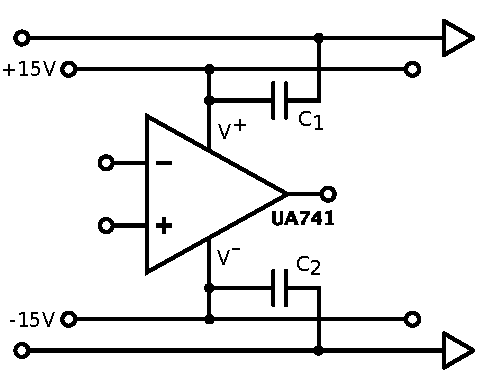
\includegraphics[width=6cm]{../E01/latex/alimentazione.pdf}}
 \caption{Grafico dell'alimentazione dell'OPAMP. La tensione di alimentazione è fornita con il generatore di tensione costante, mentre le capacità sono $C_1=(0.112 \pm 0.001)$ \si{\micro\farad} $C_2=(0.095\pm0.001)$ \si{\micro\farad}. Per maggiore chiarezza negli schemi circuitali, questa configurazione sarà nascosta negli schemi successivi, ma comunque presente sulla breadboard.}
 \label{gr:costante}
\end{figure}

Inoltre, al fine di evitare problemi di rumore durante l'alimentazione, abbiamo collegato l'alimentazione a due capacità come nello schema in Figura \ref{gr:costante}.

\section{Generatore di corrente}

In questo circuito abbiamo assemblato un generatore di corrente costante, cioè un dispositivo in grado di erogare una corrente costante ai capi di una resistenza (che definiremo \textit{resistenza di carico} $R_c$), indipendentemente dal valore di quest'ultima. Per valutare questa caratteristica abbiamo dunque utilizzato come $R_c=R_2$ una resistenza variabile di tipo \textit{trimmer}. Lo schema circuitale è in Figura \ref{gen_continua}.

\begin{wrapfigure}[21]{r}{0.55\textwidth}
  \begin{center}
    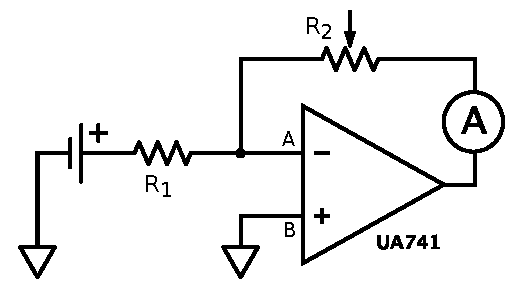
\includegraphics[width=0.40\textwidth]{../E01/latex/c1.pdf}
  \end{center}
  \caption{Schema del generatore di corrente costante. Come valori abbiamo utilizzato $R1=(3.85 \pm 0.01)$ \si{\kilo\ohm} e $V_{gen}=3.85$ \si{\volt}, mentre $R_2$ è variabile. Come amperometro è utilizzato il multimetro, mentre per alimentare l'OPAMP e come generatore di tensione costante in figura, abbiamo utillizzato il generatore Agilent E3631A.}
  \label{gen_continua}
\end{wrapfigure}

Risolviamo ora il circuito, considerando la tensione fornita dal generatore di tensione continua come $V_{gen}$ e la tensione in uscita dall'OPAMP come $V_{out}$. Dato che B si trova a potenziale di comune, per (\ref{eq:regola_V}) anche A sarà allo stesso potenziale, che considereremo nullo. Dunque varranno
\begin{equation}
V_{gen} - V_A = V_{gen} = I_1 R_1
\label{eq:gen_1}
\end{equation}
$$V_A-V_{out} = -V_{out} = I_2 R_2$$
Per (\ref{eq:regola_I}) e la legge di Kirkhhoff sui nodi, avremo invece che la corrente passante per la resistenza di carico è uguale alla corrente di (\ref{eq:gen_1}). Dunque $I=I_1=I_2$.

Otteniamo dunque che la tensione di output si modificherà, ad opera dell'OPAMP, in modo da far passare sempre lo stesso valore di corrente attraverso $R_2$; ciò avviene per il fenomeno di retroazione negativa, che ci permette di controllare la tensione di output tramite la resistenza di feedback, che in questo caso è $R_2$, e di ottenere dunque una corrente costante passante per il circuito di feedback. Imponendo l'uguaglianza della corrente possiamo inoltre trovare il valore della tensione di uscita

$$V_{out}=-\frac{R_2}{R_1} V_{gen}$$

Durante l'esperienza abbiamo però deciso di misurare la corrente passante per la resistenza piuttosto che la tensione di uscita, ponendo un amperometro fra l'uscita dell'OPAMP e la resistenza di carico $R_2$. Come valore di corrente abbiamo scelto $1$ \si{\milli\ampere}, discostandoci dalla corrente massima in cui l'amplificatore operazionale potrebbe non comportarsi più in maniera ideale ($10/20$ \si{\milli\ampere}); e avendo a disposizione una resistenza $R_1=(3.85 \pm 0.01)$ \si{\kilo\ohm}, per (\ref{eq:gen_1}), abbiamo utilizzato una tensione continua di $3.85$ \si{\volt}. Di seguito proponiamo alcuni valori sperimentali che confermano la capacità del circuito da noi creato di fornire alla resistenza di carico una corrente costante di $1$ \si{\milli\ampere}.

\begin{center}
\begin{tabular}{c|c|c|c|c|c|c|c|c}
Resistenza variabile [\si{\ohm}] & 0.54 & 35.1 & 412 & 1021 & 1996 & 3068 & 4170 & 4719 \\ 
\hline 
Corrente nel carico [\si{\milli\ampere}] & 1.002 & 1.002 & 1.002 & 1.002 & 1.002 & 1.002 & 1.002 & 1.002 \\ 
\end{tabular}
\end{center}

Gli errori sulla tabella sono uguali, cioè unitari sull'ultima cifra del valore, sia per le resistenza che per le correnti.

\section{Sommatore Pesato}

\subsection{Circuito}

Valutiamo ora il sommatore pesato, cioè un circuito che dati alcuni segnali in ingresso (due nel nostro caso) li somma con relativi pesi dati dal rapporto fra la resistenza di feedback ($R_f$) e quella a loro associata ($R_1$ e $R_2$). Lo schema circuitale è in Figura \ref{sommatore_pesato}.

\begin{wrapfigure}[21]{l}{0.55\textwidth}
  \begin{center}
    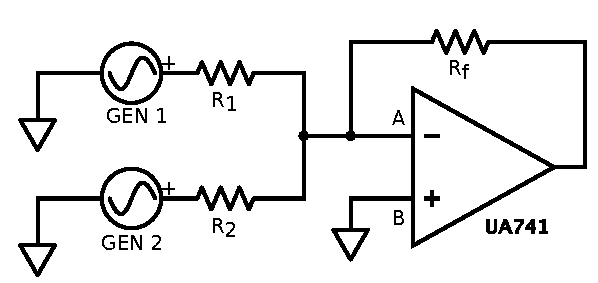
\includegraphics[width=0.40\textwidth]{../E01/latex/c2.pdf}
  \end{center}
  \caption{Schema del sommatore pesato. Come valori abbiamo utilizzato $R_f=(99.7 \pm 0.1)$ \si{\kilo\ohm}, $R_1=(99.9 \pm 0.1)$ \si{\kilo\ohm} e $R_2=(49.8 \pm 0.1)$ \si{\kilo\ohm}, dove per $R_2$ è stato necessario utilizzare un parallelo di due resistenza da $100$ \si{\kilo\ohm}. Come GEN 1 abbiamo utilizzato l'oscilloscopio, mentre per GEN 2 il generatore di forme d'onda. Infine, per valutare la tensione in uscita abbiamo utilizzato l'oscilloscopio.}
  \label{sommatore_pesato}
\end{wrapfigure}

Per risolvere il circuito consideriamo, definendo le tensioni dei generatori 1 e 2 rispettivamente $V_1$ e $V_2$, le seguenti equazioni derivanti dalle leggi di Kirkhhoff e dalla (\ref{eq:regola_I})
$$V_1 - V_A =I_1 R_1 \qquad V_2 - V_A =I_2 R_2$$
$$V_A - V_{out} =(I_1+I_2) R_f$$
Per (\ref{eq:regola_V}) vale inoltre che $V_A=V_B=0$; dunque otteniamo, sostituendo le correnti nell'ultima equazione sopra
$$V_{out}=-R_f \left( \frac{V_1}{R_1}+\frac{V_2}{R_2}\right)$$

Si può dunque definire un peso relativo $\phi_i$ ad ogni segnale dato dal rapporto fra $R_f$ ed $R_{i}$ (con $i=1,2$) e scrivere una formula del tipo
$$V_{out}=-\sum^{2}_{i=1} \frac{R_f}{R_{i}}V_{i}=-\sum^{2}_{i=1} \phi_i V_{i}$$

Durante l'esperienza abbiamo optato per valori semplici dei rapporti fra le resistenze, utilizzando i seguenti valori: $R_f=R_1=100 k\Omega$ e $R_2=50 k\Omega$. Si ottengono dunque $\phi_1=1$ e $\phi_2=2$.

\subsection{Grafici}

Presentiamo ora i grafici di alcune forme d'onda in uscita.

$$$$

\begin{figure}[ht]
 \centering
   {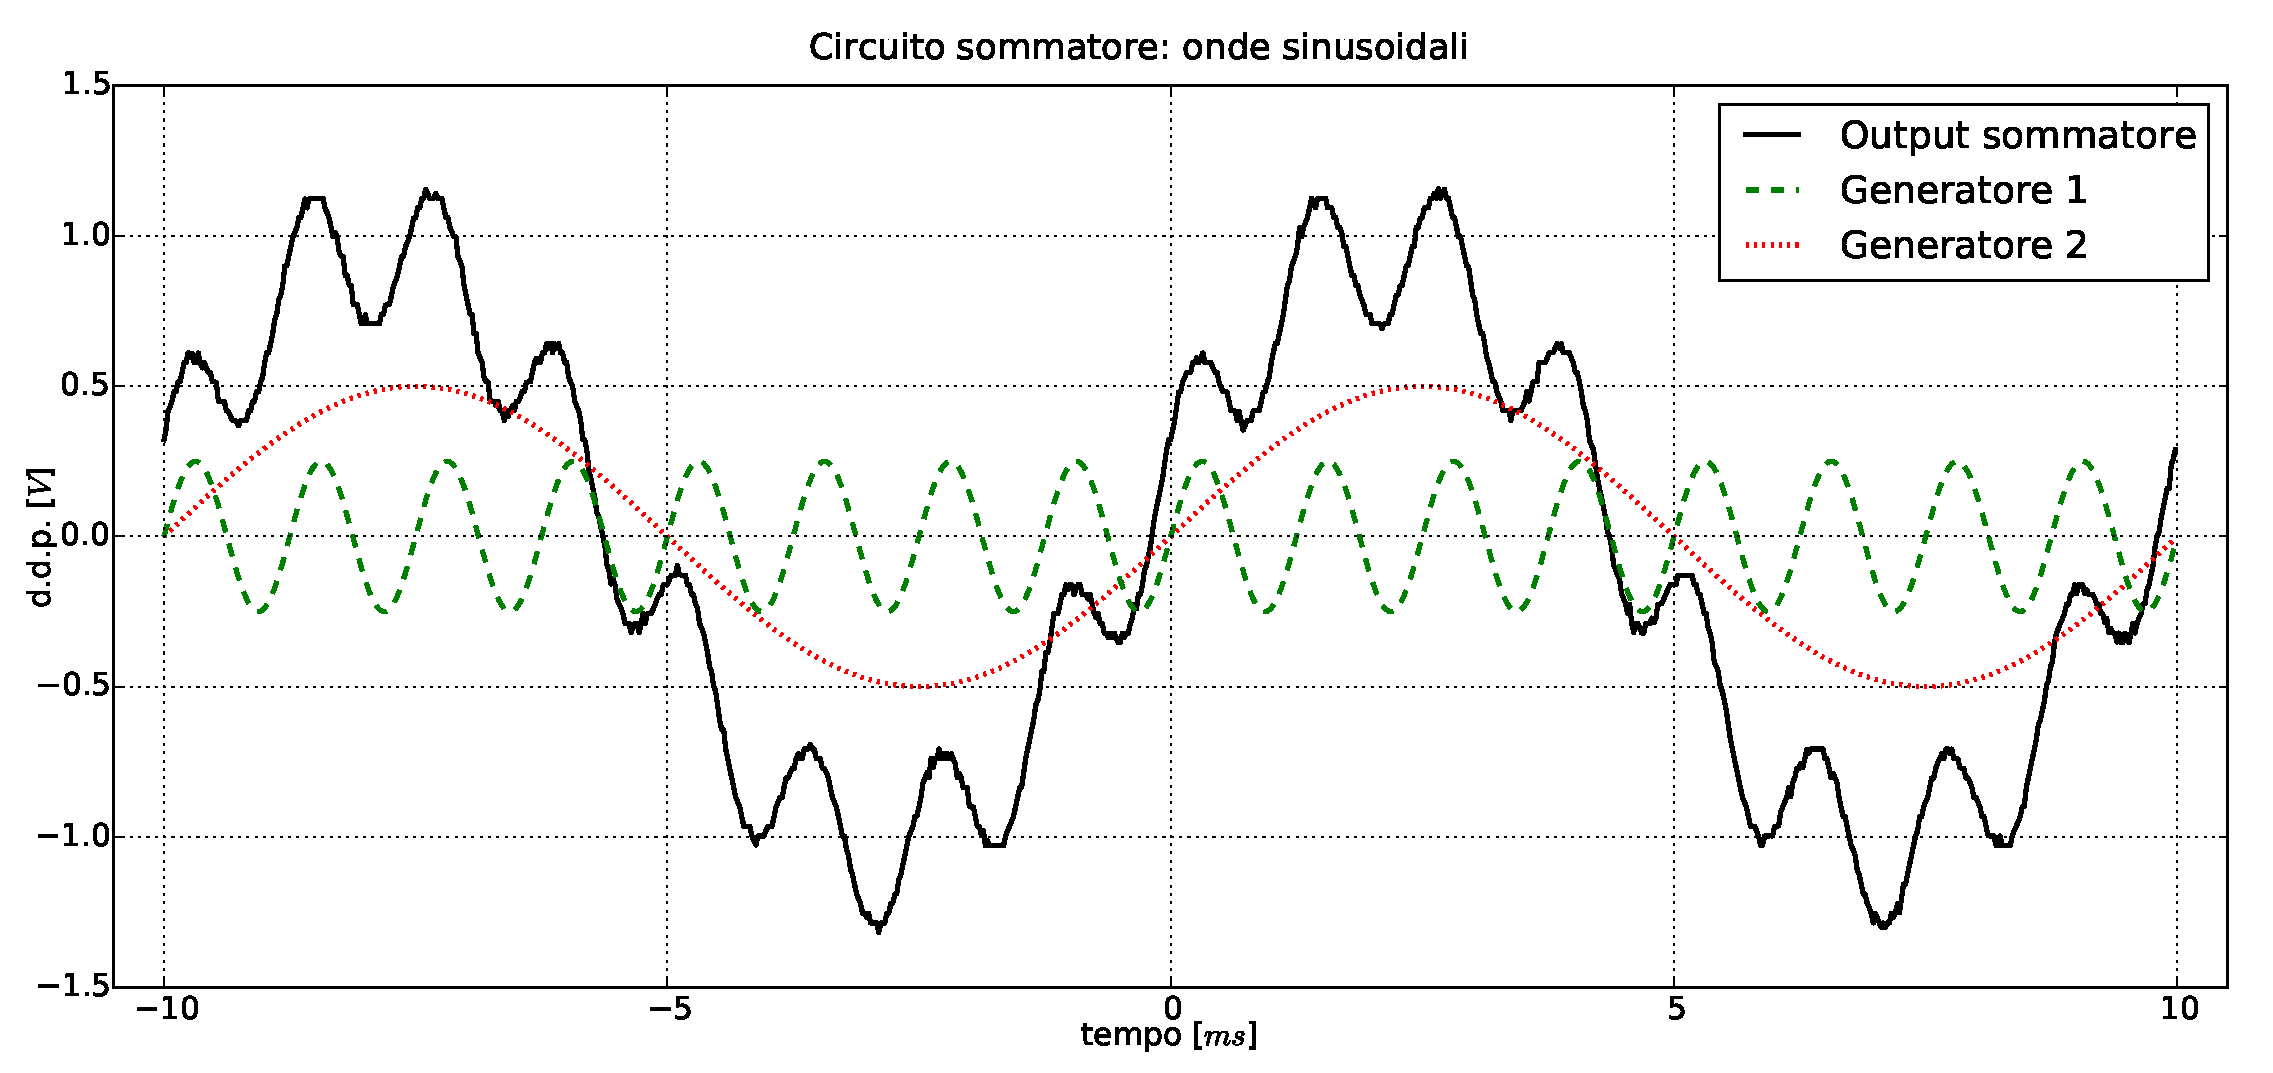
\includegraphics[width=16.5cm]{../E01/latex/sinsin.pdf}}
 \caption{Grafico della tensione di uscita. Il generatore 1 (generatore dell'oscilloscopio) crea un'onda sinusoidale di $\nu=800$ \si{\hertz} e $V^1_{pp}=500$ \si{\milli\volt}; il generatore 2 (generatore di forme d'onda) crea invece un'onda sinusoidale di $\nu=100$ \si{\hertz} e $V^2_{pp}=1000$ \si{\milli\volt}. Notiamo inoltre che l'ampiezza massima è pari a $\phi_1 V^1_{pp}+\phi_2 V^2_{pp}=2500$ \si{\milli\volt}.}
 \label{gr:onde1}
\end{figure}

$$$$

\begin{figure}[ht]
 \centering
   {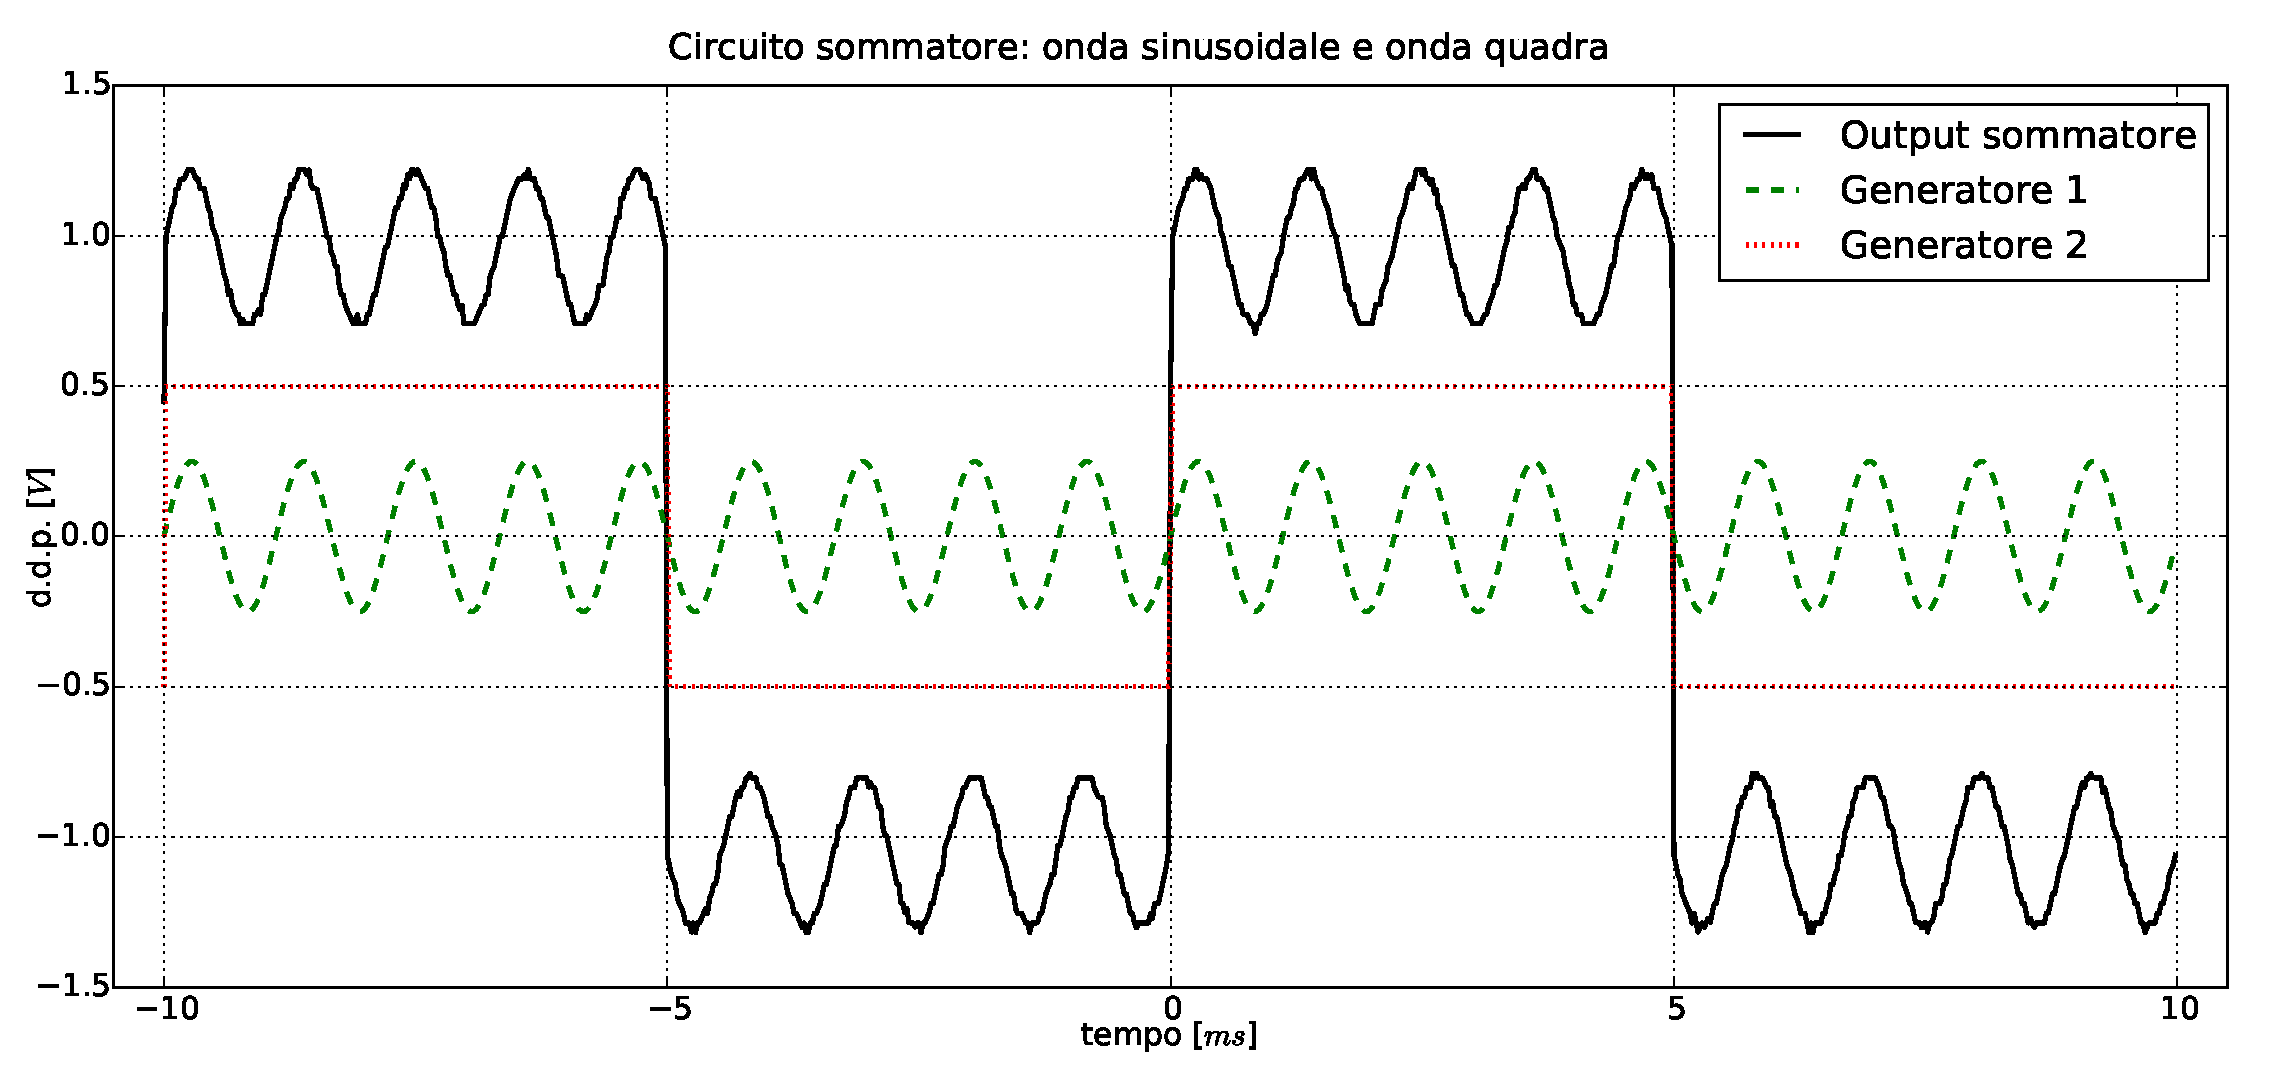
\includegraphics[width=16.5cm]{../E01/latex/sinquad.pdf}}
 \caption{Grafico della tensione di uscita. Il generatore 1 (generatore dell'oscilloscopio) crea un'onda sinusoidale di $\nu=900$ \si{\hertz} e $V^1_{pp}=500$ \si{\milli\volt}; il generatore 2 (generatore di forme d'onda) crea invece un'onda quadra di $\nu=100$ \si{\hertz} e $V^2_{pp}=1000$ \si{\milli\volt}. Notiamo inoltre che anche in questo caso l'ampiezza massima è pari a $\phi_1 V^1_{pp}+\phi_2 V^2_{pp}=2500$ \si{\milli\volt}.}
 \label{gr:onde2}
\end{figure}

\subsection{Battimenti}

Utilizzando due forme d'onda sinusoidali con il sommatore, abbiamo potuto il battimento, fenomeno che si verifica quando la differenza fra le frequenze delle onde in ingresso è sufficientemente bassa.

Con due onde abbiamo che:
$$V_{out}=\phi_1 A_1 \sin [2 \pi \nu_1 t + \theta_1] + \phi_2 A_2 \sin [2 \pi \nu_2 t + \theta_2]$$

Supponiamo che $A=\phi_1 A_1=\phi_2 A_2$, come nel caso del grafico sotto riportato. Utilizzando le formule di prostaferesi otteniamo che

$$V_{out}=2A \sin \left[4 \pi (\nu_1 + \nu_2) t + \frac{\theta_1+\theta_2}{2}\right] \cos \left[4 \pi (\nu_1 - \nu_2)t + \frac{\theta 1-\theta_2}{2}\right]$$


\begin{figure}[ht]
 \centering
   {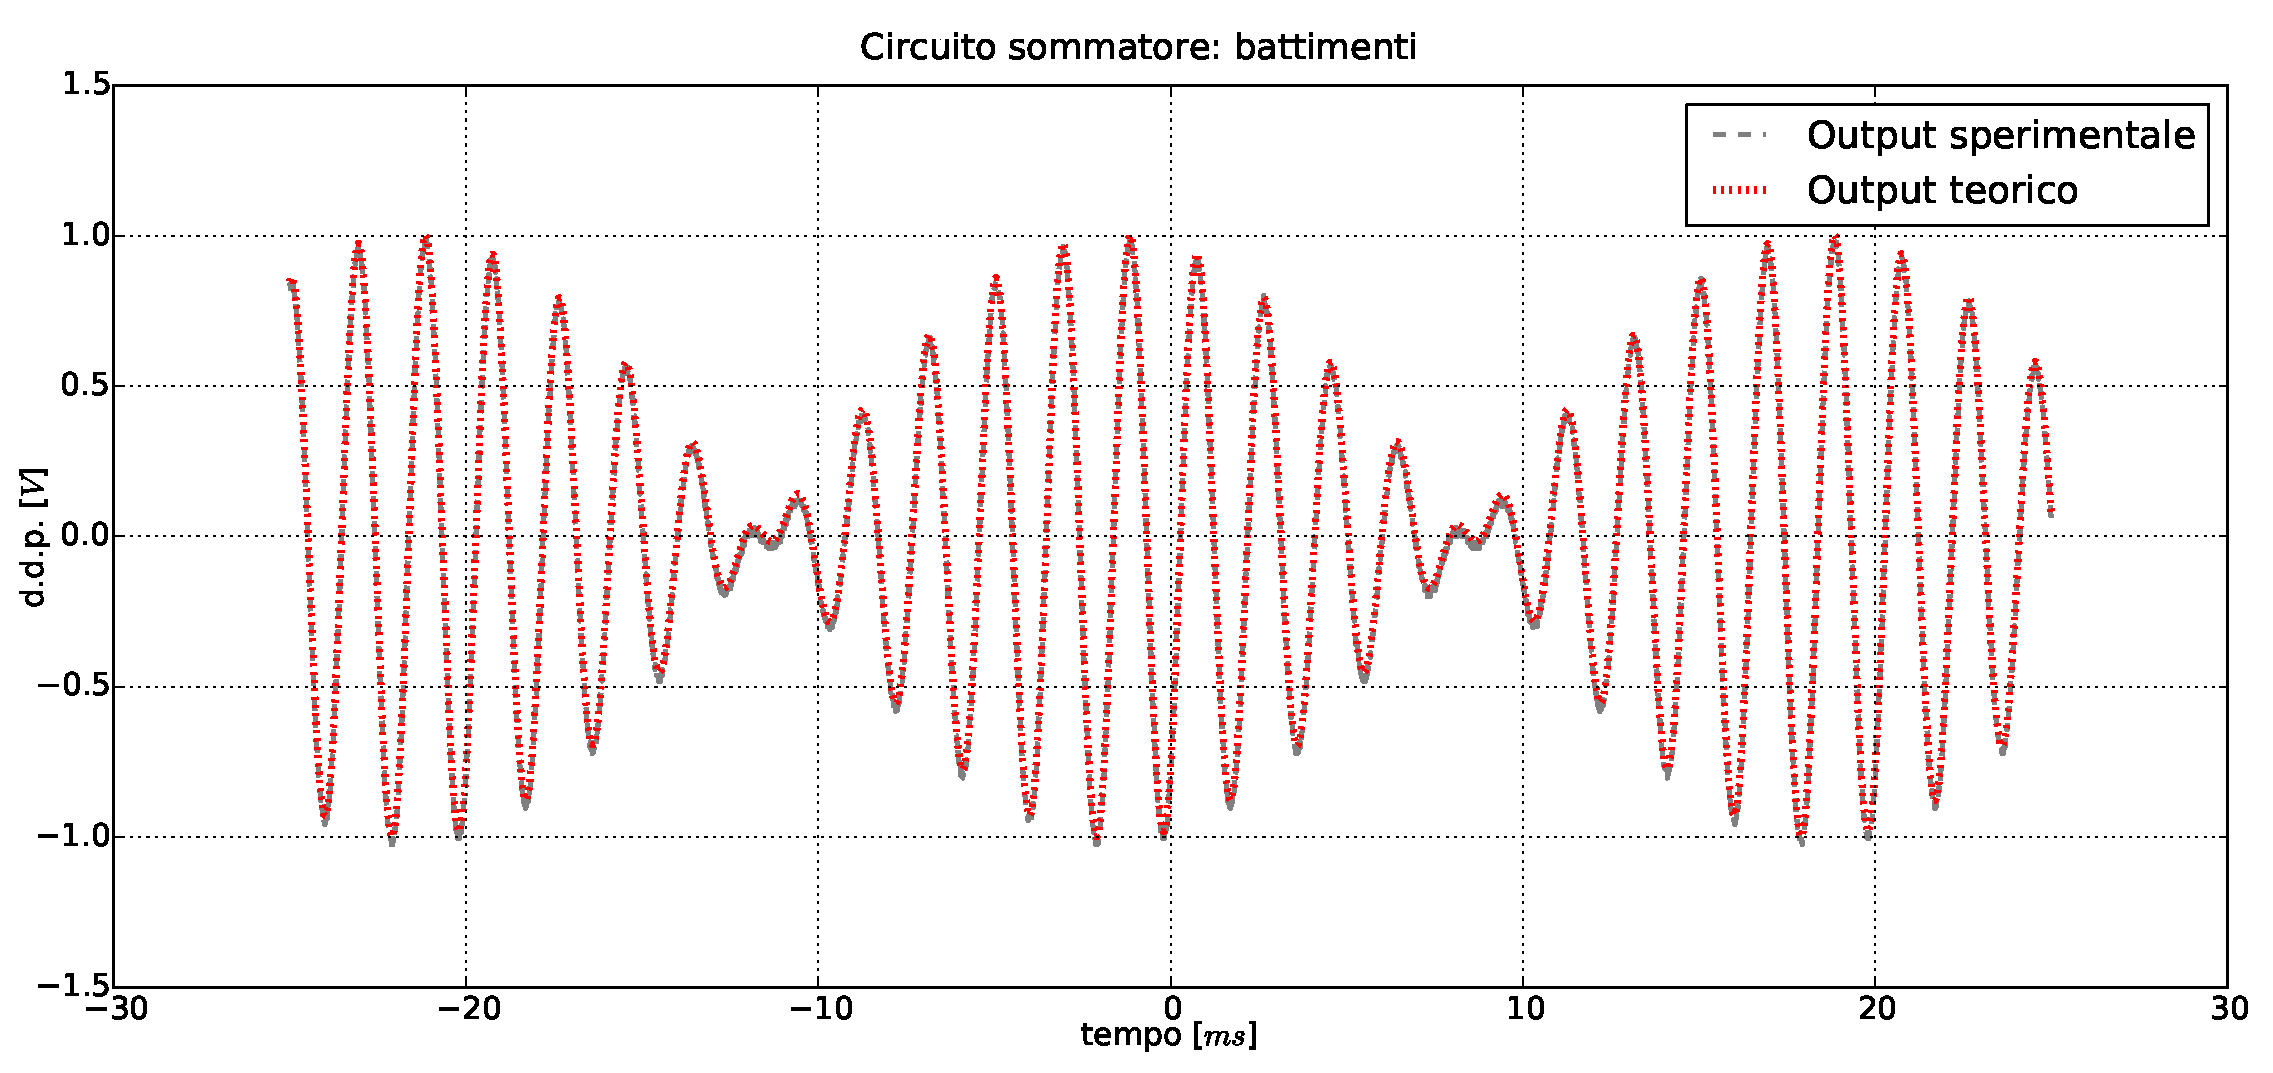
\includegraphics[width=17.5cm]{../E01/latex/battimenti_ideali.pdf}}
 \caption{Grafico della tensione di uscita. Il generatore 1 (generatore dell'oscilloscopio) crea un'onda sinusoidale di $\nu=900$ \si{\hertz} e $V^1_{pp}=500$ \si{\milli\volt}; il generatore 2 (generatore di forme d'onda) crea invece un'onda quadra di $\nu=100$ \si{\hertz} e $V^2_{pp}=1000$ \si{\milli\volt}. Notiamo inoltre che anche in questo caso l'ampiezza massima è pari a $\phi_1 V^1_{pp}+\phi_2 V^2_{pp}=2500$ \si{\milli\volt}.}
 \label{gr:battimenti}
\end{figure}

\newpage

% COMANDI PER AZZERARE IL CONTEGGIO DI FORMULE O FIGURE DA QUESTO PUNTO

%\setcounter{section}{0}
%\setcounter{figure}{0}
%\setcounter{equation}{0}

\setcounter{footnote}{0}

\section{24.09.2014 - Amplificatori operazionali reali}

Scopo di questa esperienza è quello di studiare un amplificatore operazionale $\mu$A741.
Ne analizzeremo l'offset e le correnti di polarizzazione (\textit{bias currents}) cercando di stimarne un valore, tramite circuiti progettati ad hoc.
Premettiamo che il circuito di alimentazione è lo stesso utilizzato nella precedente esperienza e dunque non ripeteremo le considerazioni e gli schemi circuitali già proposti.
Inoltre ricordiamo che la circuiteria di alimentazione sugli schemi è stata nascosta per facilitarne la comprensione.

\subsection{Strumenti e materiali}

\begin{itemize} [noitemsep]
\item Generatore di tensione continua Agilent E3631A (max $\pm \, \SI{25}{\volt}$ o $\pm \, \SI{6}{\volt}$);
\item Multimetro Agilent 34410A a sei cifre e mezza;
\item Un amplificatore operazionale $\mu$A741;
\item Resistenze e capacità di vari valori;
\item un trimmer a un giro da \SI{5}{\kilo\ohm} e uno da \SI{10}{\kilo\ohm};
\item un trimmer multigiro da \SI{10}{\kilo\ohm};
\item Breadboard e cablaggi vari.
\end{itemize}

\subsection{Stima e correzione dell'offset}
\label{par2:offset}

In questa prima parte dell'esperienza tratteremo il problema dell'offset. In un amplificatore ideale sappiamo che quando sia ingresso invertente che ingresso non invertente sono collegati a comune il segnale in uscita è nullo. Ciò è dovuto alla perfetta simmetria interna dell'op-amp. Ovviamente nel mondo reale non è possibile realizzare tale fatto in quanto non si riescono a costruire transistor BJT con specifiche identiche. 

\subsubsection{Configurazione senza retroazione}

Quando colleghiamo entrambi gli ingressi a comune l'op-amp vede all'ingresso una differenza di potenziale (ovviamente, fra gli ingressi non c'è, in quanto collegati entrambi a comune) la quale viene amplificata dal guadagno a maglia aperta: come $V_{out}$ avremo dunque un valore diverso da zero. Nel nostro caso l'op-amp andava in saturazione negativa (\SI{-14.3}{\volt}). Ricordando il funzionamento di un amplificatore operazionale, possiamo dire che il circuito si comporta come se la tensione all'ingresso invertente fosse maggiore di quella all'ingresso non invertente. Inoltre il valore $V_{out}$ è diverso da \SI{-15}{\volt} utilizzati come alimentazione in quanto il valore di tensione massimo $|V_{out}|$ è leggermente inferiore a $|V^-|$. In Figura(\ref{cir:open_loop}) è riportato lo schema del circuito utilizzato.

\begin{figure}[ht]
        \centering
        \begin{subfigure}[b]{0.35\textwidth}
                 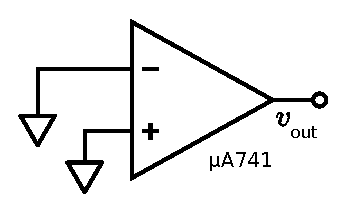
\includegraphics[width=0.70\textwidth]{../E02/latex/open_loop.pdf}
                \caption{Circuito a maglia aperta}
                \label{cir:open_loop}
        \end{subfigure}%
    \quad
        \begin{subfigure}[b]{0.35\textwidth}
               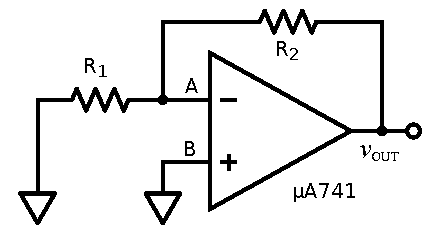
\includegraphics[width=0.70\textwidth]{../E02/latex/inv.pdf}
                \caption{Circuito amplificatore}
                \label{cir:inv}
        \end{subfigure}
     
\end{figure}

Con il circuito in Figura (\ref{cir:open_loop}) non possiamo quindi ricavare una stima del valore di offset. Per fare ciò dobbiamo ricorrere a un circuito amplificatore come quello in Figura(\ref{cir:inv}) (invertente o non invertente), che ci permetta di controllare il guadagno.

\subsubsection{Configurazione con retroazione}

Trattiamo per primo il caso \textbf{invertente}. Assumiamo nel punto A la presenza di un generatore di tensione $V_A=V_{off}$ e consideriamo $V_B=0$. Vale allora che, uguagliando le correnti

$$\frac{V_{off}}{R_1} + \frac{V_{off}-V_{out}}{R_2} = 0$$

da cui si ricava che
$$V_{out}=\left(1+\frac{R_2}{R_1}\right) V_{off}$$

Analogamente si tratta il caso \textbf{non invertente}. Per far ciò immaginiamo nel punto B un generatore di tensione $V_B=-V_{off}$ . Si ottiene lo stesso risultato ricavato per il caso \textbf{invertente}.

%I valori nominali delle componenti circuitali utilizzate sono: $R_1=\SI{120}{\ohm}$ e $R_2=\SI{10/100}{\kilo\ohm}$.

Riportiamo nella seguente tabella i valori di offset calcolati, definendo il guadagno = $1+\frac{R_2}{R_1}$. 

\begin{center}
\begin{savenotes}
\begin{tabular}{c|c|c|c|c|c|c}
$R_1[\si{\ohm}]$ & $R_2[\si{\kilo\ohm}]$ & Gain &$V_{out} [\si{\milli\volt}]$ & $V_{off}$ [\si{\milli\volt}]\\ 
\hline 
$119.8\pm0.1$ & $9.911\pm0.001$ & $83.73\pm0.07$&  $-103.5 \pm 0.5$ & $-1.23 \pm0.01$\\
\hline
$119.8\pm0.1$ & $99.35\pm0.01$ & $830.3\pm0.7$ &$ -1025 \pm 2$ & $-1.2 \pm0.1$\\

\end{tabular}
\end{savenotes}
\end{center}

\begin{wrapfigure}[17]{l}{0.55\textwidth}
  \begin{center}
    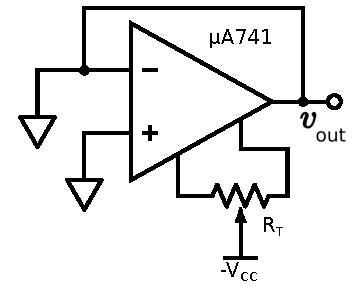
\includegraphics[width=0.280\textwidth]{../E02/latex/trimmer_correction.pdf}
  \end{center}
  \caption{Circuito a guadagno unitario, con trimmer sui piedini 1 e 5 dell'OPAMP per compensare l'offset.}
  \label{cir2:trimmer}
\end{wrapfigure}

%Come sappiamo la tensione di offset non è però l'unico problema che incontriamo quando usiamo op-amp reali. Infatti ingresso invertente e non invertente sono collegati alle basi di transistor e, ovviamente, per polarizzarli serve una corrente di base. Gli effetti di tale corrente si sommeranno dunque a quelli dovuti all'offset. Tale argomento sarà comunque trattato approfonditamente nella sezione successiva. 

Per risolvere il problema dell'offset possiamo servirci di una resistenza variabile ($trimmer$) che posizioneremo tra i piedini 1 e 5 dell'op-amp, collegandola a $V^-$. Regolando tale resistenza andremo a generare una contro tensione che bilancerà l'offset. Il circuito utilizzato per verificare il bilanciamento dell'offset è quello in Figura \ref{cir2:trimmer}.

Durante l'esperienza abbiamo utilizzato un trimmer multigiro da \SI{10}{\kilo\ohm}, con il quale abbiamo raggiunto la tensione $V_{out}\simeq 0\si{\volt}$. Come verifica abbiamo misurato la tensione $V_{out}$ a maglia aperta, ottenendo il valore $V_{out}=1.3\pm0.2$. Ricordando che il guadagno $A_{ol}$ è di 100-120dB, si nota il buon bilanciamento della tensione di offset.

\begin{wrapfigure}[17]{r}{0.55\textwidth}
  \begin{center}
    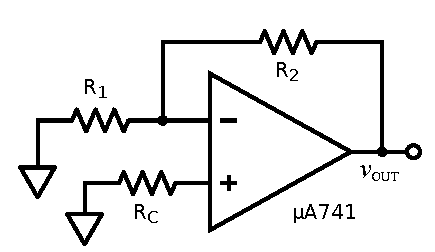
\includegraphics[width=0.280\textwidth]{../E02/latex/current_correction.pdf}
  \end{center}
  \caption{Circuito utilizzato per la stima di $V_{off}$ con la correzione sulle correnti data da $R_C$.}
  \label{cir2:current_correction}
\end{wrapfigure}

Come sappiamo attraverso gli ingressi invertente e non invertente dell'amplificatore operazionale reale scorrono delle correnti, dette di bias. Queste, per quanto piccole (\si{\nano\ampere}), hanno comunque un contributo sull'offset totale. Per minimizzare il loro impatto sul valore della tensione di offset abbiamo inserito fra l'ingresso non invertente e comune una resistenza di compensazione $R_C$ tale da annullare il contributo delle correnti di offset sulla tensione di uscita.

Il contributo alla tensione di uscita data dalle correnti di polarizzazione, supponendo già l'offset compensato, è

\begin{equation}
V_{out}^{C} = \left( 1+\frac{R_2}{R_1} \right)\left[ \frac{I_{b^-}R_2}{\frac{R_1+R_2}{R_1}} - I_{b^+} R_C\right]
\label{eq2:Vout_currents}
\end{equation}

dalla quale, se $|I_{b^+}|\simeq|I_{b^-}|$ e $V_{out}^{C}=0$, banalmente otteniamo

$$R_C=\frac{1}{\frac{1}{R_1} + \frac{1}{R_2}} $$



Riportiamo nella seguente tabella i nuovi valori in questa nuova configurazione (circuito in Figura \ref{cir2:current_correction}):

\begin{center}
\begin{tabular}{c|c|c|c|c|c|c}
$R_C [\si{\ohm}]$& $R_1[\si{\ohm}]$ & $R_2[\si{\kilo\ohm}]$ & Gain & $V_{out}' [\si{\milli\volt}]$ & $V_{off}' [\si{\milli\volt}]$ & $|V_{off}-V_{off}'|[\si{\milli\volt}]$ \\ 
\hline 
$119.4\pm0.1$ & $119.8\pm0.1$ & $9.911\pm0.001$  & $83.73 \pm 0.07$ & $-105.5 \pm 0.5$ & $-1.26 \pm0.01$ & $0.02\pm0.01$ \\
\hline
$119.4\pm0.1$ & $119.8\pm0.1$ & $99.35\pm0.01$  & $830.3\pm0.7$ &$ -1038 \pm 5$ & $-1.2 \pm 0.1$ & $\approx 0$\\
\end{tabular}
\end{center}

Notiamo che le differenze fra i valori della tensione di offset con e senza $R_C$ sono compatibili con il rumore ambientale (qualche decina di \si{\micro\volt} di ampiezza). Se osserviamo la tensione $V_{out}$ nei casi con e senza resistenza $R_C$, notiamo una differenza di circa $13\si{\milli\volt}$. Nel successivo paragrafo stimeremo una corrente di bias di $37\si{\nano\ampere}$. Possiamo dunque osservare che la caduta di potenziale su tale resistenza dovuta alla corrente di polarizzazione è $\Delta V \simeq 3 \si{\milli\volt}$. Tale valore è circa 4 volte più piccolo della differenza delle tensioni in uscita misurate. Nella stima dell'offset abbiamo dunque il contributo delle correnti di bias ma essendo dello stesso ordine di grandezza del rumore ambientale (o addirittura inferiore) non possiamo valutarne quantitativamente gli effetti. 

\subsection{Correnti di polarizzazione}

\begin{wrapfigure}[12]{r}{0.55\textwidth}
  \begin{center}
    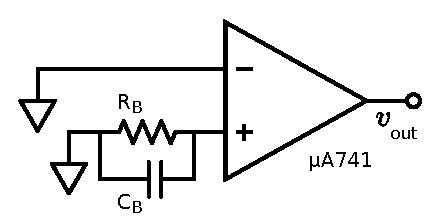
\includegraphics[width=0.30\textwidth]{../E02/latex/direct_measure.pdf}
  \end{center}
  \caption{Schema del circuito non retro-azionato utilizzato per stimare la corrente di polarizzazione. La resistenza utilizzata è $R_B=10.36\pm0.01$\si{\mega\ohm}; la capacità $C_B=102 \pm 1$ \si{\nano\farad}.}
  \label{circuito:rel2_correnti_senzaretroazione}
\end{wrapfigure}


Nella seconda parte dell'esperienza abbiamo misurato le correnti di polarizzazione che scorrono nei due ingressi. Ricordiamo che la tensione di offset è già stata compensata dall'esterno con l'utilizzo di un \textbf{trimmer}. 

\subsubsection{Misura diretta}





Come primo approccio abbiamo tentato una misura diretta della corrente $I_{b^+}$.
Abbiamo utilizzato una resistenza molto grande (10\si{\mega\ohm}) prima dell'ingresso non invertente (analogamente si può fare con l'ingresso invertente) e abbiamo misurato la tensione ai suoi capi. La legge di ohm ci assicura che $I_{b^+}=\frac{V}{R}$. A causa del rumore di fondo però il valore misurato non era stabile. Si è dunque pensato di aggiungere in parallelo alla resistenza un condensatore, così da stabilizzare la tensione.




%Per far ciò, dato che attendevamo una corrente dell'ordine dei \si{\nano\ampere}, abbiamo utilizzato una resistenza molto grande in modo da poter leggere il valore della tensione su una scala accettabile per il multimetro.

%Durante la procedura abbiamo però notato che, a causa di rumori ambientali, il valore di tensione sul multimetro fluttuava sulla prima cifra, rendendo nostra misurazione ovviamente non quantitativa (al massimo poteva stimarci l'ordine di grandezza della corrente). Per ovviare, abbiamo inserito in parallelo alla resistenza un condensatore che caricandosi si portava alla stessa ddp dei capi della resistenza. In questo modo abbiamo potuto ottenere un valore meno fluttuante, che si attestava a $V=(-80 \pm 2)$ \si{\milli\volt}, cioè $I_{b^+}=(7.7 \pm 0.2)$ \si{\nano\ampere}.

Il valore che siamo riusciti a stimare con la stabilizzazione con condensatore è $V=(-80 \pm 2) \si{\milli\volt} \Rightarrow I_{b^+}=(7.7 \pm 0.2)$ \si{\nano\ampere}.


%Con questo metodo semplice abbiamo potuto ottenere una prima stima del valore della corrente. Di contro bisogno considerare che il rumore non permette di avere una stima qualitativa ed inoltre la resistenza, scaldandosi, modifica il suo valore e potrebbe portare ad un errore sulla misura. Successivamente progetteremo dunque un circuito che, sfruttando l'amplificazione data dall'amplificatore operazionale, minimizzerà questi errori.

I difetti di tale metodo di misura sono molteplici. Anzitutto la resistenza si scalda e ciò produce un aumento della resistenza stessa ($\approx 5 ppm/^{\circ}C$).





\subsubsection*{Misura di $I_{b^-}$}

\begin{wrapfigure}[15]{l}{0.55\textwidth}
  \begin{center}
    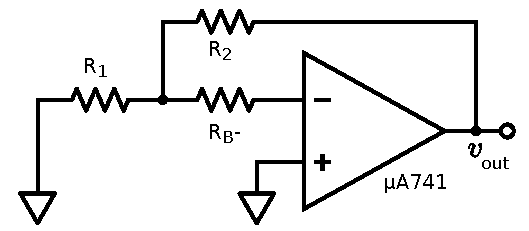
\includegraphics[width=0.30\textwidth]{../E02/latex/inv_current.pdf}
  \end{center}
  \caption{Schema del circuito retro-azionato utilizzato per stimare la corrente di polarizzazione $I_{b^-}$. Le resistenze utilizzate sono $R_1=(98.9\pm0.1)$ \si{\ohm}, $R_2=(99.4\pm0.1)$ \si{\kilo\ohm} e $R_B=(99.4\pm0.1)$ \si{\kilo\ohm}.}
  \label{circuito:rel2_correnti_retroazione_inv}
\end{wrapfigure}

Come secondo approccio abbiamo dunque provato una misura indiretta della corrente $I_{b^-}$. Per fare ciò abbiamo utilizzato il circuito in Fig. \ref{circuito:rel2_correnti_retroazione_inv}. Ricordiamo che la tensione di offset è già stata compensata esternamente.

%Chiamiamo $V_{-}$ la tensione al capo di $R_B$ collegato all'OPAMP e $V^*$ quello opposto, vale in quel punto la legge di Kirchhoff sui nodi
Chiamiamo $V_{inv}$ la tensione all'ingresso invertente e $V_{nodo}$ la tensione nel nodo in cui sono collegate tra loro $R_B$,$R_1$ e $R_2$. Basta ora risovere il seguente sistema 


$\begin{cases} \frac{V_{nodo} - V_{in}}{R_1} + \frac{V_{nodo}-V_{out}}{R_2} + \frac{V_{nodo}-V_{inv}}{R_B}=0 \\ V_{in}=V_{inv}=0  \\I_{b^-} = \frac{V_{nodo}}{R_B} \end{cases} $

Da cui segue dopo alcuni calcoli algebrici

%$$\frac{V_{nodo} - V_{in}}{R_1} + \frac{V_{nodo}-V_{out}}{R_2} + \frac{V_{nodo}-V_{inv}}{R_B}=0$$

%Per la struttura del circuito e la compensazione dell'offset è immediato vedere che $V_{in}=V_{inv}=0$ e, se definiamo la corrente $I_{b^-} = \frac{V_{nodo}}{R_B}$):

$$I_{b^-}=\frac{V_{out}}{R_2 R_B}\frac{1}{\frac{1}{R_1}+\frac{1}{R_2}+\frac{1}{R_B}}$$

Le resistenze sono state dimensionate in modo da ottenere tensioni $V_{out}$ dell'ordine del Volt.
La misura di tensione di uscita è di $(3.89\pm0.02)\si{\volt} \Rightarrow I_{b^-} = (38 \pm 5)$ \si{\nano\ampere}.

\subsubsection*{Misura di $I_{b^+}$}

\begin{wrapfigure}[17]{r}{0.55\textwidth}
  \begin{center}
    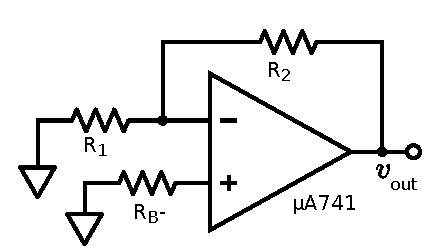
\includegraphics[width=0.25\textwidth]{../E02/latex/ninv_current.pdf}
  \end{center}
  \caption{Schema del circuito retro-azionato utilizzato per stimare la corrente di polarizzazione $I_{b^+}$. Le resistenze utilizzate sono le medesime del circuito precedente in Figura \ref{circuito:rel2_correnti_retroazione_inv}.}
  \label{circuito:rel2_correnti_retroazione_noninv}
\end{wrapfigure}

%Similmente a quanto visto per la configurazione prima, troviamo che, data la legge di Kirchhoff (con $V^*$ la tensione all'ingresso non invertente, che per quanto detto sopra è uguale a quella all'ingresso invertente)

In questo secondo caso riportato in Fig. \ref{circuito:rel2_correnti_retroazione_noninv} chiamiamo $V_{ninv}$ la tensione all'ingresso non invertente.


$\begin{cases}\frac{V_{ninv} - V_{in}}{R_1} + \frac{V_{ninv}-V_{out}}{R_2}=0 \\ I_{b^+}=\frac{V_{ninv}}{R_B}\\ V_{in}=0 \end{cases}$

Risolvendo il sistema otteniamo


\begin{equation}
I_{b^+}=\frac{V_{out}}{R_2 R_B}\frac{1}{\frac{1}{R_1}+\frac{1}{R_2}}
\label{eq2:corrente_noninv}
\end{equation}

Anche in questo caso le resistenze sono state dimensionatein modo da ottenere un $V_{out}$ dell'ordine dei Volt. La misura di tensione di uscita è di $-(3.72 \pm 0.02) \si{\volt} \Rightarrow I_{b^+} = - (37.2 \pm 0.2)$ \si{\nano\ampere}

Ricordiamo che il segno della corrente dipende dalla convenzione scelta. Abbiamo deciso di assumere nei calcoli segno positivo per correnti entranti e segno negativo per correnti uscenti. La corrente $I_{b^-}$ sarà dunque entrante nell'ingresso inverntente mentre $I_{b^+}$ sarà uscente dall'ingresso invertente.

%\footnote{ La negatività della corrente è intesa rispetto all'ingresso non invertente, ed è quindi uscente rispetto a tale ingresso. Al contrario, nel paragrafo precedente, la corrente è intesa entrante nel punto di $V^*$, e quindi è entrante rispetto all'ingresso invertente.}.

\subsubsection*{Calcolo di $I_{b^+}$ data $I_{b^-}$}

Proviamo a calcolare $I_{b^+}$ utilizzando il valore di $I_{b^-}$ calcolato sopra e avvalendoci di Eq. (\ref{eq2:Vout_currents}). \'E triviale ricavare la seguente identità: 

$$I_{b^+} = \frac{R_1}{R_B(R_1+R_2)}(I_{b^-} R_2-V_{out})$$

Inserendo i valori numerici otteniamo $I_{b^+} = - (37.2 \pm 0.2)$ \si{\nano\ampere}, compatibile con il risultato precedente.


\subsubsection*{Cenni sul rumore termico}
Nel paragrafo sulla misura diretta della corrente di bias abbiamo ottenuto un valore non compatibile con quello stimato utilizzando la procedura indiretta. Proviamo a vedere se tale discrepanza può essere dovuta al rumore termico.
 
Consideriamo la larghezza di banda del multimetro $\Delta f = \SI{1}{\hertz}$ e siano $k_B = \SI{1.38e-23}{\joule\per\kelvin}$ la costante di Boltzmann, $T$ la temperatura assoluta e $R$ il valore della resistenza presa in considerazione

\begin{equation}
	V_{eff}^2 = 4 k_B T R \Delta f
\end{equation}

Inserendo i valori numerici e il valore di resistenza $R=\SI{10}{\mega\ohm}$ si ottiene che il rumore termico è 5 ordini di grandezza inferiore alla tensione misurata.

\begin{equation}
	V_{eff} = \sqrt{4 k_B T R \Delta f} \simeq 4 \times 10^{-7} \si{\volt}
\end{equation}






\subsection{Conclusioni}
In questa esperienza abbiamo studiato le caratteristiche di un OPAMP, misurandone tensione di offset e correnti di polarizzazione. La presenza dell'offset può essere bilanciata utilizzando semplicemente un trimmer collegato a 2 piedini dell'amplificatore operazionale. Così facendo possiamo creare una contro-tensione interna che bilancia automaticamente l'offset. Le correnti di polarizzazione, invece, possono essere bilanciate ottimizzando le impedenze in ingresso. Tuttavia, essendo dell'ordine dei \si{\nano\ampere}, giocano un ruolo solo nel caso si lavori con tensioni di pochi millivolt. Negli utilizzi più comuni (con tensioni dell'ordine dei Volt) possono essere trascurate.




%In questa esperienza abbiamo potuto osservare come gli OPAMP, sebbene siano dei circuiti abbastanza precisi, abbiano delle imperfezioni, date dalla loro composizione circuitale (sono presenti dei transistor BJT al loro interno).
%Le discrepanze tra il modello ideale e l'OPAMP reale sono date principalmente dallo sbilanciamento della risposta dello stesso ($V_{offset}$) e dalle correnti di polarizzazione (\textit{bias currents}).
%Per nostra fortuna spesso gli OPAMP presentano dei connettori predisposti a minimizzare la tensione di offset con circuiti di compensazione: nel nostro caso un trigger collegato ai piedini di offset e all'alimentazione negativa.
%Una volta bilanciato l'opamp, abbiamo misurato le correnti di polarizzazione e abbiamo potuto osservare che esse sono dell'ordine dei \si{\nano\ampere}, quindi trascurabili per gli utilizzi più comuni.


\newpage

\setcounter{footnote}{0}

\section{30.09.2014 - Amplificatori Operazionali Reali - Seconda Parte}

In questa esperienza abbiamo studiato ulteriori caratteristiche che distinguono l'opamp reale dal modello ideale.
Più precisamente abbiamo analizzato e misurato lo \textit{slew rate}, la massima corrente pilotabile, la larghezza di banda passante e il guadagno a maglia aperta $A_{ol}$ di un opamp $\mu$A741.

Ricordiamo che in ogni schema sono stati sottintesi la circuitazione di alimentazione (cavi e capacitori) e quella dedicata al bilanciamento dell'offset (cavi e trimmer).

\subsection*{Strumenti e materiali}

\begin{itemize} [noitemsep]
\item Oscilloscopio Agilent DSO-X 2002A (bandwidth \SI{70}{\mega\hertz}, sample rate \num{2} GSa/s);
\item Generatore di tensione continua Agilent E3631A (max $\pm \, \SI{25}{\volt}$ o $\pm \, \SI{6}{\volt}$);
\item Generatore di forme d'onta Agilent 33120A con range di frequenza da \SI{100}{\micro\hertz} a \SI{15}{\mega\hertz};
\item Multimetro Agilent 34410A;
\item Un amplificatore operazionale $\mu$A741;
\item Resistenze e capacità di vari valori;
%\item un trimmer (potenziometro);
\item Breadboard e cablaggi.
\end{itemize}

\subsection{Misura dello Slew Rate}

\begin{wrapfigure}[15]{r}{0.55\textwidth}
  \begin{center}
    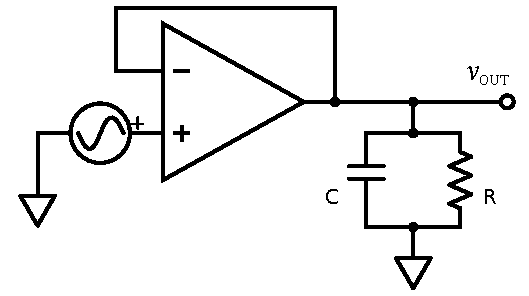
\includegraphics[width=0.30\textwidth]{../E03/latex/slew_rate.pdf}
  \end{center}
  \caption{Schema del circuito utilizzato per stimare lo Slew Rate. La resistenza utilizzata è $R=(2.17\pm0.01)$ \si{\kilo\ohm}; la capacità $C=(200 \pm 10)$ \si{\pico\farad}.}
  \label{cir3:slew_rate}
\end{wrapfigure}

Uno dei parametri che caratterizzano l'amplificatore operazionale è lo Slew Rate, definito come
$$SR = \mathrm{max}\left[\frac{\Delta V}{\Delta t}\right]$$
che indica la velocità massima con cui l'amplificatore operazionale può far variare la tensione in uscita nell'unità di tempo. Ciò significa che, per segnali in entrata con derivata temporale superiore ad SR dell'OPAMP, avremo un segnale distorto in uscita.

Nel nostro caso abbiamo utilizzato un generatore caratterizzato da uno Slew Rate di $SR_{gen}=\SI{315}{\volt\per\micro\second}$ per creare il segnale in ingresso (onda quadra) e valutato la forma d'onda del segnale in uscita utilizzando il circuito in Figura \ref{cir3:slew_rate}.
Dati i diversi ordini di grandezza fra $SR_{gen}$ e il valore atteso di $SR$ ($\approx \SI{0.5}{\volt\per\micro\second} $) possiamo considerare il generatore come avente uno slew rate pressoché infinito.
La capacità è utilizzata come serbatoio di cariche per attenuare fenomeni di rumore nel segnale creati dal generatore.

\begin{figure}[ht]
 \centering
   {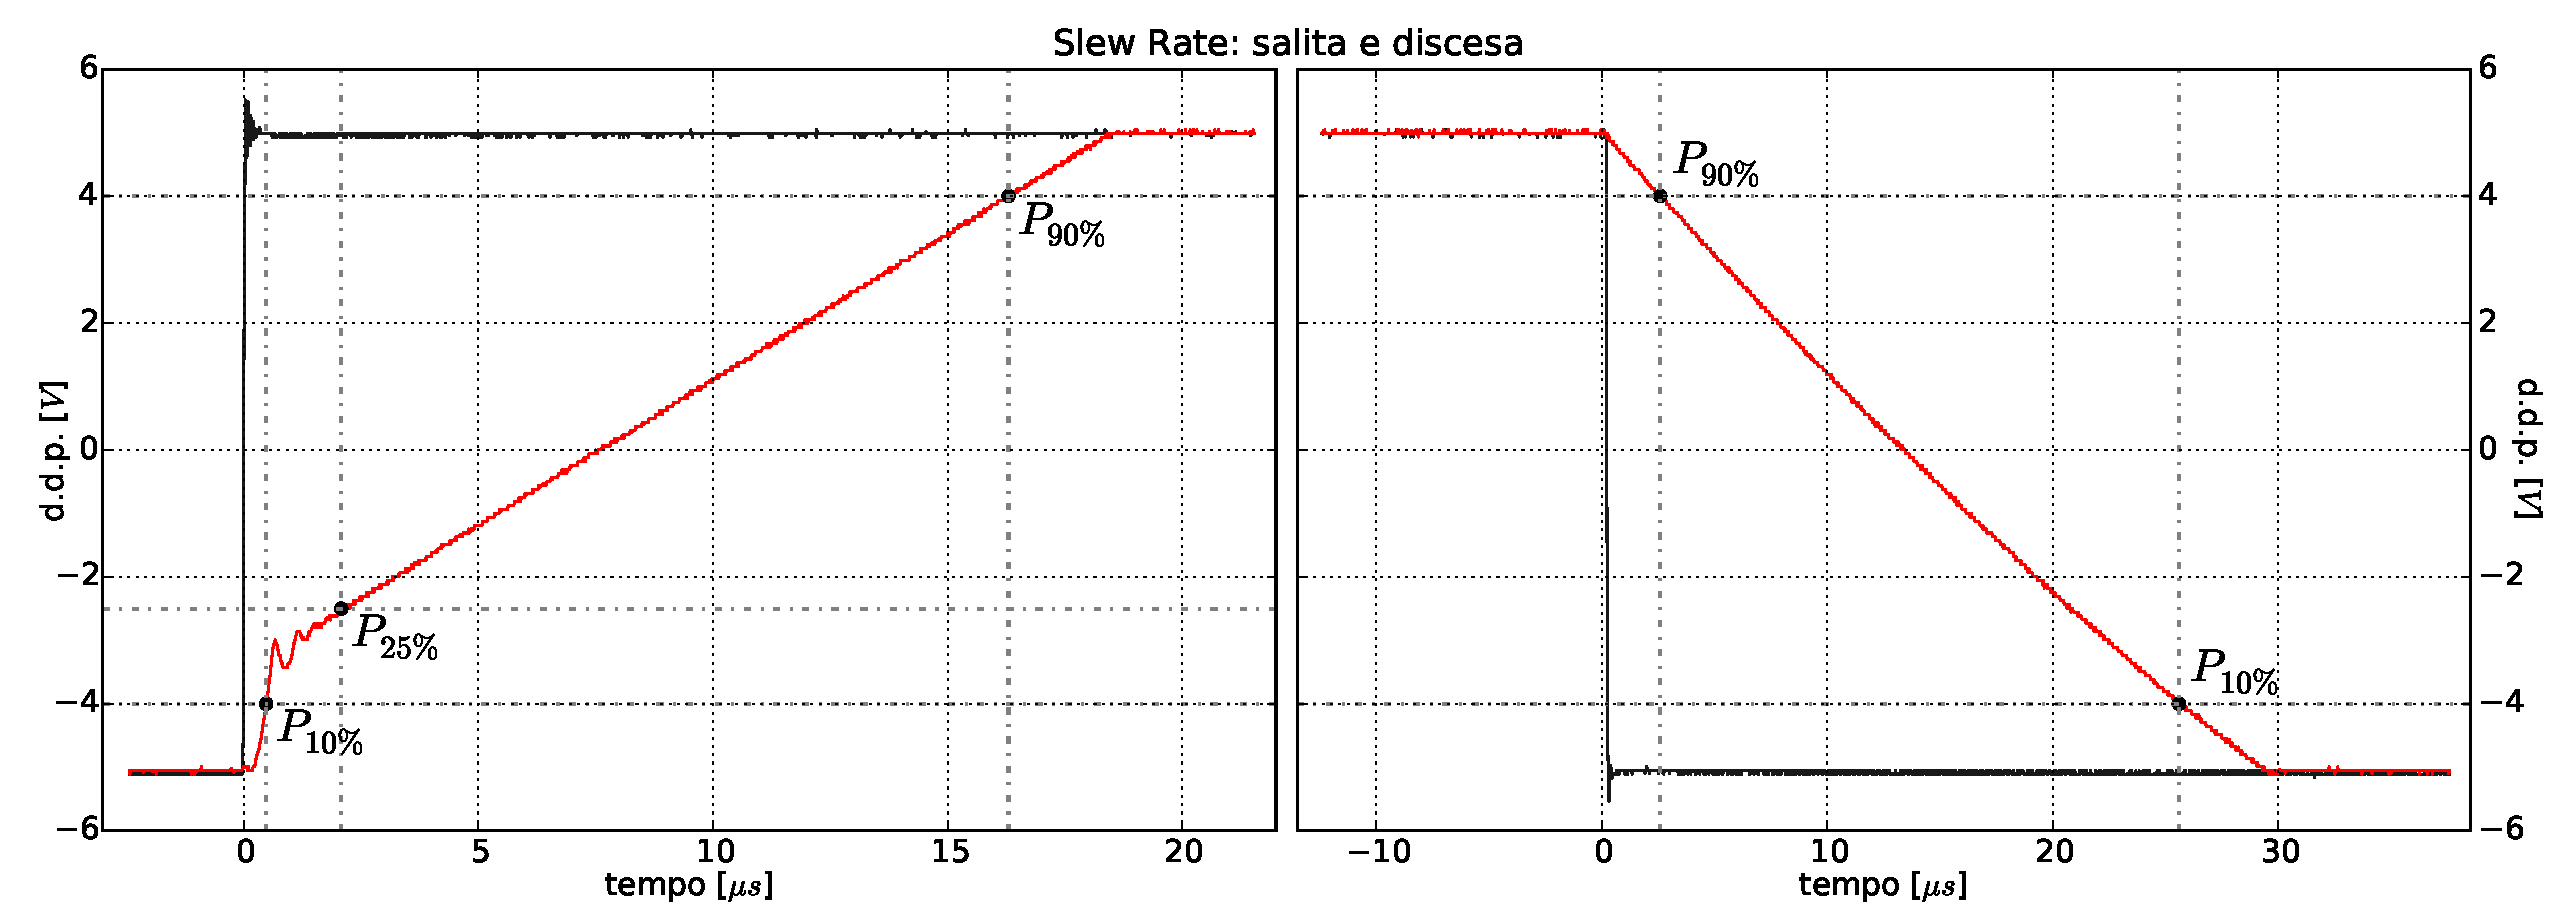
\includegraphics[width=\textwidth]{../E03/latex/sr_uad.pdf}}
 \caption{Grafico della tensione in uscita (rosso) ed in entrata (nero) in funzione del tempo. I $\Delta$ sono relativi alle differenze fra le coordinate dei punti segnati.}
 \label{gr3:slew_rate}
\end{figure}

Inizialmente abbiamo posto la frequenza a $f=1$\si{\kilo\hertz} e la tensione picco picco a $V_{pp}=10$ \si{\volt}; con la funzione cursore dell'oscilloscopio abbiamo poi misurato $\Delta V = (8.07 \pm 0.01)$ \si{\volt} fra il 10\% e il 90\% del valore di tensione picco picco in uscita e la relativa $\Delta t = (15.9 \pm 0.1)$ \si{\micro\second}, ottenendo uno $SR=(0.507 \pm 0.003)$ \si{\volt\per\micro\second}.

Come però si può vedere dal grafico in Figura \ref{gr3:slew_rate} si nota che nella parte vicina al 10\% è presente una parte di segnale affetta da rumore che potrebbe rendere poco precisa la nostra misura. Infatti siamo interessati al rapporto fra i $\Delta$; dunque portare il limite inferiore ad un valore percentuale più alto, dato il rumore, rende più precisa la misura. Portando dunque la percentuale del limite inferiore al 25\% abbiamo ottenuto i seguenti valori: $\Delta V = (6.48 \pm 0.01)$ \si{\volt} e $\Delta t = (14.5 \pm 0.1)$ \si{\micro\second}, dunque $SR = (0.447 \pm 0.003)$ \si{\volt\per\micro\second}. Durante l'esperienza utilizzeremo questo valore come riferimento per lo Slew Rate del nostro amplificatore.

Abbiamo anche notato che lo Slew Rate è differente a seconda che il segnale abbia derivata $dV/dt$ positiva o negativa (grafico in Figura \ref{gr3:slew_rate}, immagine di destra). Nel secondo caso, infatti, abbiamo ottenuto i seguenti valori: $\Delta V = (8.00 \pm 0.01)$ \si{\volt} e $\Delta t = (23.2 \pm 0.1)$ \si{\micro\second}, quindi $SR = (0.345 \pm 0.004)$ \si{\volt\per\micro\second}.

\subsection{Misura della capacità di pilotaggio}

\begin{wrapfigure}[16]{l}{0.55\textwidth}
  \begin{center}
    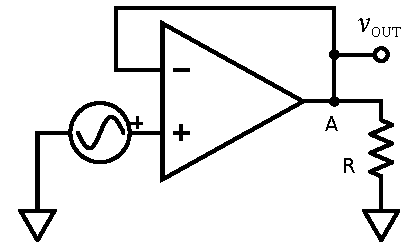
\includegraphics[width=0.26\textwidth]{../E03/latex/max_current.pdf}
  \end{center}
  \caption{Schema del circuito utilizzato per misurare la corrente massima. La resistenza utilizzata è $R=(98.47\pm0.01)$\si{\ohm}; il generatore fornisce un'onda triangolare di $f=1$ \si{\kilo\hertz} e $5 V_{pp}$.}
  \label{cir3:max_current}
\end{wrapfigure}

L'amplificatore operazionale ha un valore massimo di corrente erogabile in uscita. Dunque, se montiamo un circuito di feedback come in Figura \ref{cir3:max_current}, la tensione massima ai capi di $R$ sarà fissata dalla corrente massima e dal valore della resistenza stessa, da questa relazione:
\begin{equation*}
	I_{max} = \frac{V_{clip}}{R}
\end{equation*}
dove $V_{clip}$ è la tensione in cui il segnale in uscita risulta tagliato rispetto a quello in ingresso (fenomeno del \textit{clipping}).

Per misurare $I_{max}$ abbiamo dunque sfruttato questo fatto, ponendo una resistenza di carico fra l'uscita dell'operazionale e terra\footnote{Si noti che, data l'alta impedenza in ingresso dell'oscilloscopio (\SI{1}{\mega\ohm}), non era possibile misurare la corrente massima con questo strumento (attesa, come da specifiche del costruttore, sui \SI{15}{\milli\ampere}): sarebbe servita una tensione di \SI{15000}{\volt}!}, con l'oscilloscopio ai capi di tale resistenza per la misura di tensione (circuito in Figura \ref{cir3:max_current}).

\begin{figure}[ht]
 \centering
   {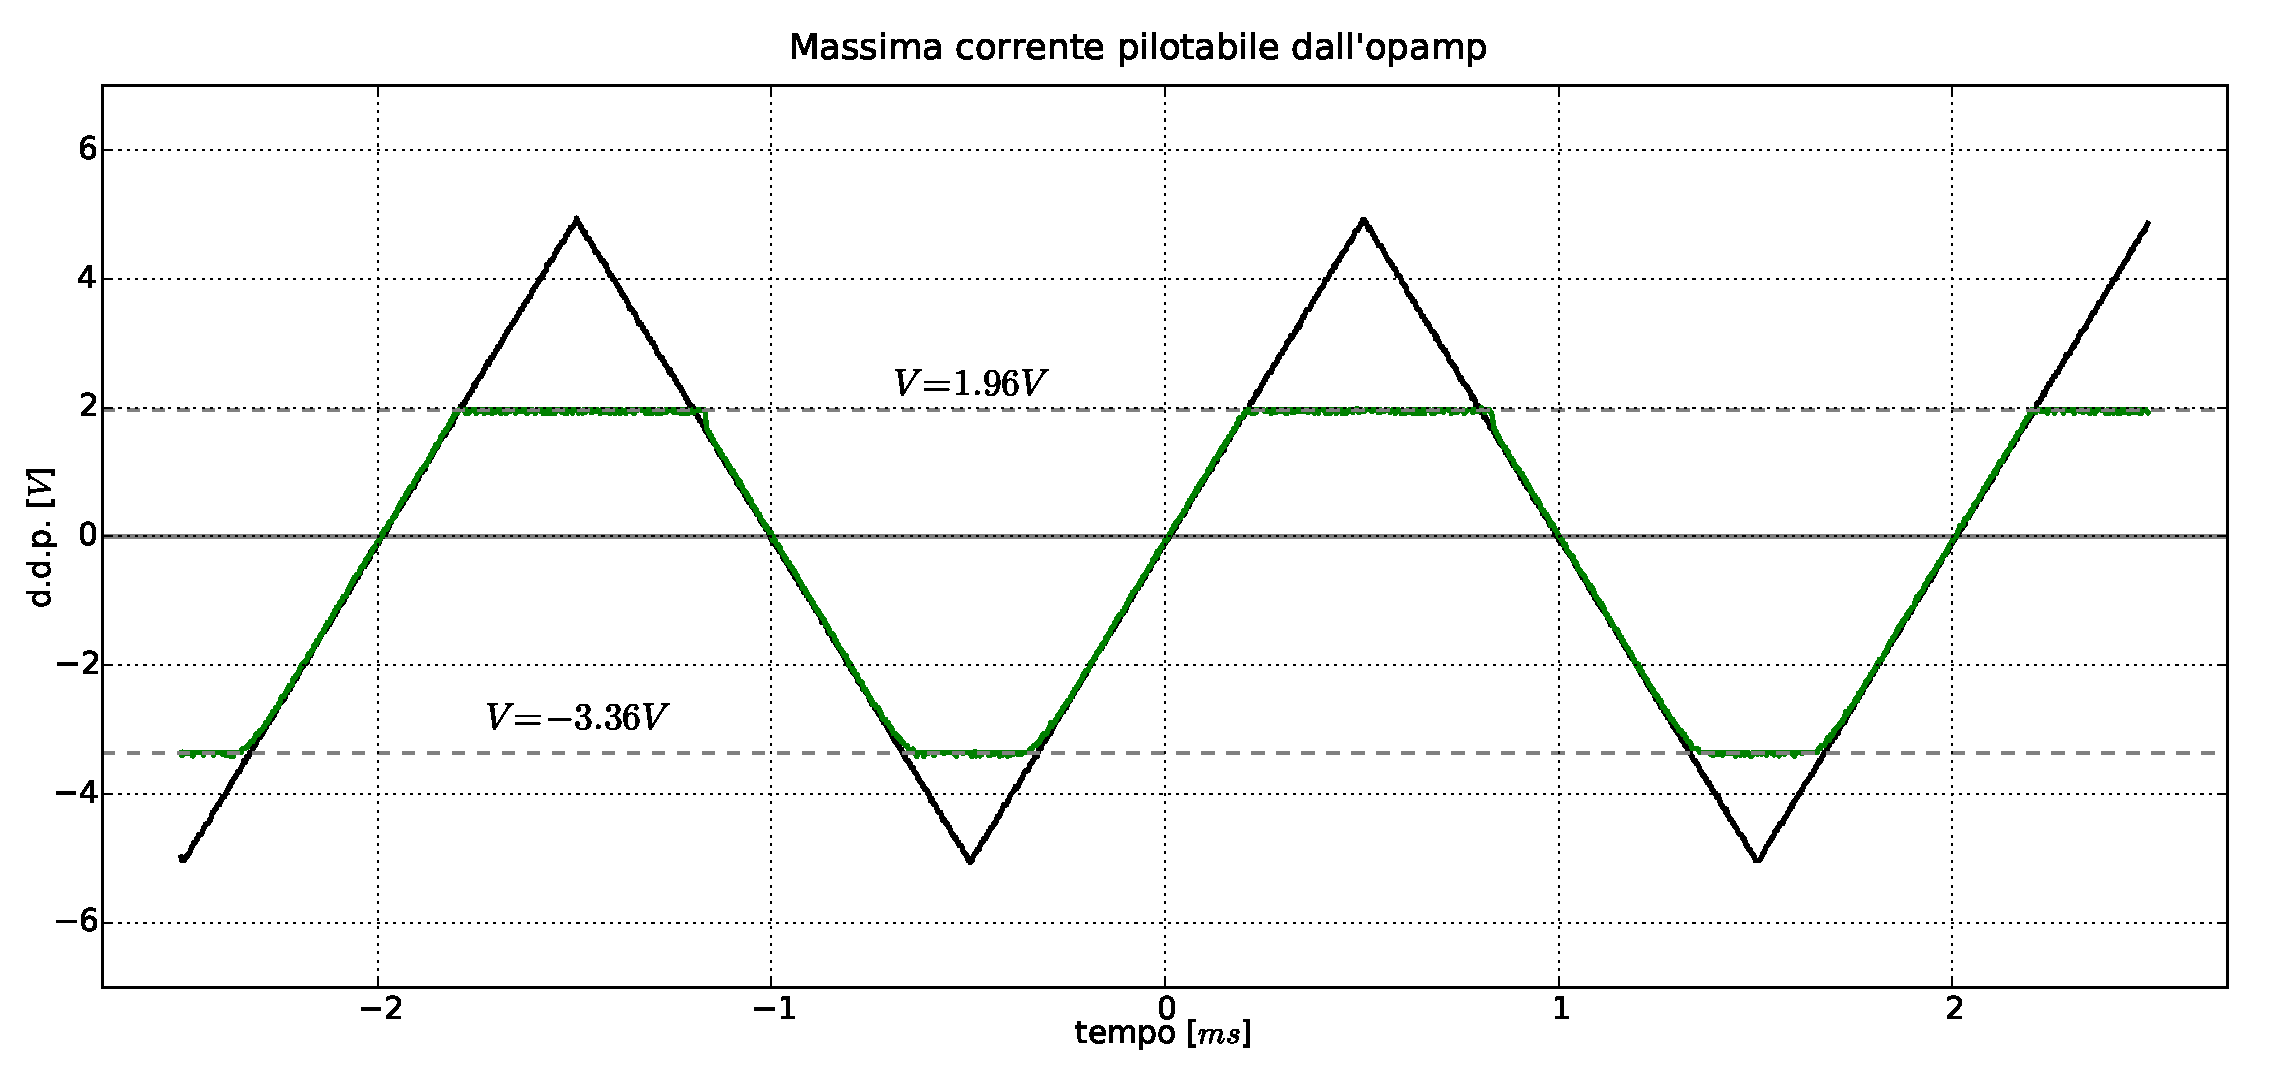
\includegraphics[width=\textwidth]{../E03/latex/clip.pdf}}
 \caption{Grafico della tensione in uscita (verde) ed in entrata (nero) in funzione del tempo. Si nota subito l'asimmetria del clip tra tensioni positive e negative.}
 \label{gr3:clip}
\end{figure}

Bisogna però considerare che la corrente, ponendo il segnale in entrata in alternata, risulta oscillare fra valori negativi e positivi (corrente rispettivamente entrante o uscente dal punto A). Inoltre, tali valori sono differenti (si nota dal grafico in Figura \ref{gr3:clip} l'asimmetria della tensione di clip). Infatti, se consideriamo $V^+ = (1.92 \pm 0.01)$ \si{\volt} la tensione di clip positiva e $V^- = (3.45 \pm 0.01)$ \si{\volt} quella negativa, otteniamo

$$I_{V^+} = \frac{V^+}{R} = (19.5 \pm 0.1) \si{\milli\ampere}  \qquad I_{V^-} = \frac{V^-}{R} = (35.2 \pm 0.2) \si{\milli\ampere}$$

Entrambi i valori sono compatibili quelli del costruttore (valori di corrente fino a $\pm 40$ \si{\milli\ampere}). Questo fatto può essere spiegato considerando che la circuiteria interna dell'opamp è composta, come già più volte ribadito, da diversi transistor che solo idealmente possono essere tutti delle medesime ed identiche caratteristiche: ciò comporta una asimmetria che può spiegare il fenomeno.

\subsection{Verifica della banda passante}
\label{par3:bode}

In questa parte dell'esperienza vogliamo valutare la banda passante di un circuito amplificatore (non invertente) considerando che il guadagno a maglia aperta dell'amplificatore operazionale dipende della frequenza.

\subsubsection*{Funzione di trasferimento e frequenza di taglio}

Esaminiamo dapprima il circuito, calcolandone la funzione di trasferimento. Per ogni amplificatore operazionale vale
\begin{wrapfigure}[20]{l}{0.45\textwidth}
  \begin{center}
    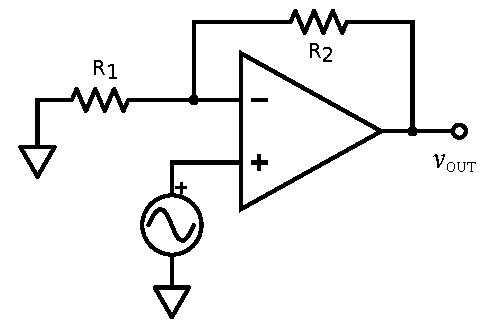
\includegraphics[width=0.32\textwidth]{../E03/latex/bandwidth.pdf}
  \end{center}
  \caption{Schema del circuito utilizzato per valutare la banda passante. La resistenza $R_1=997\pm1$ \si{\ohm} è fissa; mentre $R_2$ è stata cambiata con valori $R_2^{11\mathrm{x}}=9.91 \pm 0.01$ \si{\kilo\ohm} e $R_2^{101\mathrm{x}}=99.1 \pm 0.1$ \si{\kilo\ohm} a seconda del guadagno desiderato.}
  \label{cir3:banda}
\end{wrapfigure}
\begin{equation}
V_{out}=A(s) (V^+-V^-)
\label{eq3:regola_opamp}
\end{equation}
con il guadagno, come detto sopra, che in generale dipende da $s=j\omega$ (e quindi dalla frequenza). Consideriamo
$$V^+ = V_{in} \qquad V^-=V_{out} \frac{R_1}{R_1+R_2}$$
dove $V^-$ è ricavato dalla solita formula per l'amplificatore non invertente $(V^+-V^-)/R_1 + (V_{out}-V^-)/R_2 =0$. Definiamo
$$\beta = \frac{R_1}{R_1+R_2} = \frac{1}{G}$$
Si noti che $G$ è il guadagno circuitale di un amplificatore non invertente. Sostituendo questi valori in (\ref{eq3:regola_opamp}) otteniamo
$$A(s) V_{in} = V_{out} + V_{out} A(s) \beta$$
Calcoliamo ora la funzione di trasferimento $H$
\begin{equation}
H(s)=\frac{V_{out}}{V_{in}}=\frac{1}{\beta}\frac{1}{1+\frac{1}{A(s) \beta}}
\label{eq3:funz_trasfe}
\end{equation}
da cui è facile notare che per $A(s) \rightarrow + \infty$ (approssimazione di amplificatore ideale), $H(s)=\frac{1}{\beta}=1+\frac{R_2}{R_1}=G$, equazione che diventa indipendente dal guadagno a maglia aperta.

Schematizziamo l'OPAMP come un filtro passa basso. Abbiamo che il guadagno a maglia aperta varia con la frequenza secondo la legge
\begin{equation}
A(j\omega)=\frac{A_{ol}}{1+j\frac{\omega}{\omega_0}}
\label{eq3:passa_basso}
\end{equation}
con $\omega_0 \approx 8$ \si{\hertz} la prima frequenza di taglio dell'operazionale data dalla capacità di compensazione nella circuiteria interna e $A_{ol}$ il guadagno dell'operazionale con segnali costanti ($f = 0$). Sostituendo questo valore in (\ref{eq3:funz_trasfe}), abbiamo
\begin{equation}
H(j\omega)=\frac{\frac{A_{ol}}{1+A_{ol}\beta}}{1+j \frac{\omega}{(1+A_{ol}\beta)\omega_0}}
\label{eq3:funzione_trasferimento}
\end{equation}
da cui si nota che la nuova frequenza di taglio è data da
\begin{equation}
\omega_t=(1+A_{ol}\beta)\omega_0
\label{eq3:freq_taglio}
\end{equation}
Nel circuito in Figura \ref{cir3:banda} avevamo un guadagno $G$ retroazionato di $11$ e $101$, quindi ci aspettiamo\footnote{Questi valori sono approssimati perchè cercheremo di calcolare $A_{ol}$ con le frequenze a nostra disposizione, ricavate con l'analisi della banda, piuttosto che calcolare ora frequenze di taglio senza essere certi del valore di $A_{ol}$.} frequenze di taglio, per l'equazione precedente, rispettivamente sull'ordine dei $10^5$ e $10^4$. Per fare una stima delle frequenze di taglio era anche possibile sfruttare la costante \textit{gain-bandwidth product} GBWP $= f_t G$, costante dell'amplificatore operazionale.

\subsubsection*{Effetto dello Slew Rate}

Ovviamente, durante la misurazione bisogna minimizzare l'effetto dello Slew Rate che, come visto nel paragrafo precedente, distorce la forma d'onda in uscita. Bisogna quindi scegliere valori di tensione del segnale in ingresso appropriati.
Supponiamo dunque di avere una forma d'onda in uscita del tipo $V_{out} \sin (2 \pi f_0 t) = V_{in} G \sin (2 \pi f_0 t)$. Vale, affinché non si raggiunga lo SR
$$\mathrm{max}\left[ \frac{dV_{out}}{dt} \right] = \mathrm{max} \left[ 2 \pi V_{in} G f_0 \cos (2 \pi f_0 t) \right]= 2 \pi V_{in} G f_0 < 0.35 \si{\volt\per\micro\second}$$
dove l'ultimo valore è stato scelto per tenerci sempre abbastanza distanti dal valore reale di SR. Dunque vale che
\begin{equation}
V_{in}<\frac{0.35 \si{\volt\per\micro\second}}{2 \pi G f_0} = \frac{0.35 \si{\volt\per\micro\second}}{2 \pi \mathrm{GBWP}}
\label{eq3:tensione_max}
\end{equation}
Considerando $f_0$ come la frequenza di taglio stimata prima, otteniamo che i valori di tensione da usare nei due casi è di circa $V_{in}^{11\mathrm{x}} = 100$ \si{\milli\volt}$= V_{in}^{101\mathrm{x}}$. Si nota che la regola \ref{eq3:tensione_max} è valida quando il guadagno non dipende dalla frequenza: infatti dopo la frequenza di taglio il guadagno del circuito $G$ cala e dunque i valori di tensione ammessi risultano di valore maggiore.

\subsubsection*{Diagrammi di Bode}
\label{par3:sub_bode}

\begin{figure}[ht]
 \centering
   {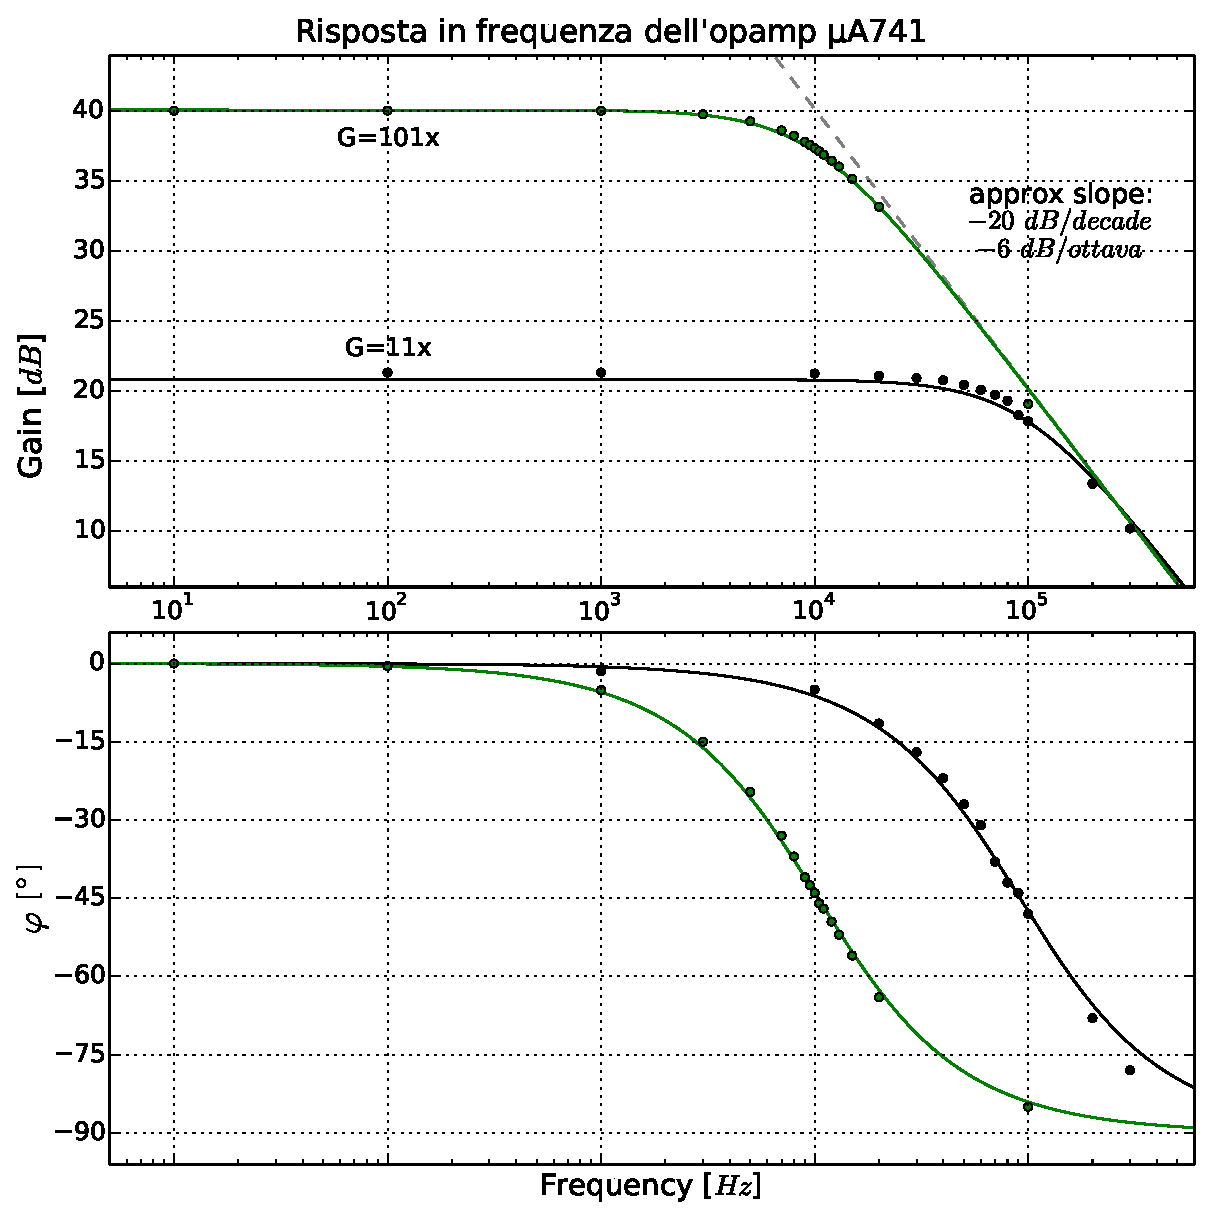
\includegraphics[width=0.75\textwidth]{../E03/latex/bode.pdf}}
 \caption{Diagrammi di Bode per il guadagno del circuito in Figura \ref{cir3:banda}. Le leggi plottate sono (\ref{eq3:fit_gain}) e (\ref{eq3:fit_fase}), con i rispettivi guadagni $G$ del circuito.}
 \label{gr3:bode}
\end{figure}

Utilizzando una forma d'onda sinusoidale abbiamo dunque misurato la tensione di uscita del circuito e la fase fra i segnali, per poi plottare i diagrammi di Bode (Figura \ref{gr3:bode}).

Dalla funzione di trasferimento (\ref{eq3:funzione_trasferimento}) possiamo inoltre trovare le relazioni fra il guadagno e la fase con la frequenza. Sappiamo infatti che il guadagno è dato $V_{out}/V_{in}$, ed in generale queste due tensioni possono essere considerate come complesse. Se siamo dunque interessati al guadagno dobbiamo considerare piuttosto il rapporto dei moduli, ed otteniamo la seguente relazione
\begin{equation}
\mathrm{Gain}=\frac{|V_{out}|}{|V_{in}|}=|H(j\omega)|=\sqrt{\frac{A_{ol}^2 \omega_0^2}{(\omega_0 + A_{ol} G \omega_0)^2 + \omega^2}}
\label{eq3:fit_gain}
\end{equation}
mentre, per la fase utilizziamo la solita formula della fase per un numero complesso (nel nostro caso $V_{out}/V_{in}$), ed otteniamo
\begin{equation}
\varphi=\arctan\left[{\frac{\mathrm{Im}[H(j\omega)]}{\mathrm{Re}[H(j\omega)]}}\right]= - \arctan\left[\frac{\omega}{(1+A_{ol}G)\omega_0}\right]
\label{eq3:fit_fase}
\end{equation}

Date queste leggi è possibile stimare $A_{ol}$ e $\omega_0$ dell'operazionale: rimandiamo al paragrafo \ref{par3:A_ol} per questi calcoli, dove saranno confrontati i valori ottenuti con questi dati e quelli presi al paragrafo \ref{par3:open}.

Infine, i valori di frequenza di taglio possono essere calcolati dalla legge al valore di fase del flesso ($45^{\circ}$). Questi sono: $f_t^{101\mathrm{x}} = (10.3 \pm 0.1)$ \si{\kHz} e $f_t^{11\mathrm{x}} = (92 \pm 1)$ \si{\kHz}, in accordo con gli ordini di grandezza stimati in precedenza.

\subsection{Guadagno Open Loop}
\label{par3:open}



In questa ultima parte dell'esperienza abbiamo cercato di misurare il guadagno $A_{ol}$ del nostro amplificatore reale.
Come sappiamo, tale guadagno è una funzione della frequenza e dobbiamo dunque trovare un modo per misurarlo.

Fino alla frequenza di circa \SI{8}{\hertz} il guadagno di un opamp $\mu$A741 è costante a circa \num{2E5}.
Oltre tale frequenza abbiamo una caduta di circa \SI{20}{\decibel}/decade.
Non risulta dunque possibile effettuare misure a loop aperto in quanto piccolissime variazioni di tensione ai due ingressi causerebbero grandi effetti in uscita.

\begin{wrapfigure}[17]{r}{0.45\textwidth}
  \begin{center}
    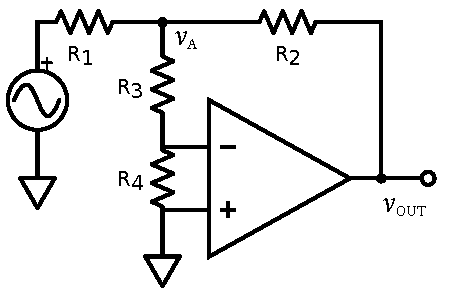
\includegraphics[width=0.280\textwidth]{../E03/latex/LF_ol.pdf}
  \end{center}
  \caption{Circuito utilizzato per misurare il guadagno $A_{ol}$. I valori di $R_4$ utilizzati sono $(5.2\pm 0.1)$ \si{\ohm},  $(9.6\pm0.1)$ \si{\ohm}, $(101.3\pm 0.1)$ \si{\ohm} e $(998.2\pm 0.1)$ \si{\ohm} mentre $R_1=\SI{98\pm1}{\kohm}$, $R_2=\SI{97\pm1}{\kohm}$ e $R_3=\SI{98\pm1}{\kohm}$.}
  \label{cir3:low_frequency}
\end{wrapfigure}

Abbiamo dunque progettato un circuito per controllare la tensione in uscita così da non mandare in saturazione il nostro opamp.
In Figura \ref{cir3:low_frequency} è riportato lo schema circuitale da noi utilizzato.
Utilizzando l'oscilloscopio abbiamo misurato i valori di tensione $V_A$ e $V_{out}$. Cerchiamo dunque di legare il guadagno a tali quantità.

Nel caso dell'amplificatore operazionale sappiamo che vale l'eq. (\ref{eq3:regola_opamp}), dove $(V_+-V_-)$ è semplicemente la differenza di potenziale presente tra i due ingressi, che sarà ovviamente data da $\Delta V = I_3R_4$, dove $I_3$ è la corrente che scorre attraverso $R_3$ ed $R_4$\footnote{Assumiamo che la corrente assorbita dagli ingressi sia trascurabile.}.
È quindi facile stimare $I_3=\frac{V_A}{R_3+R_4}$ conoscendo $V_A$.

Si ottiene dunque:
\begin{equation}
A_{ol}=\frac{{V_{out}}^{pp}}{{V_A}^{pp}} \frac{R_4+R_3}{R_4}
\label{eq3:lfgain}
\end{equation}

Osserviamo come in equazione (\ref{eq3:lfgain}) non compaia il termine $V_{in}$.
Dovremo dunque scegliere per le varie frequenze una tensione picco-picco in ingresso adeguata in modo che il nostro opamp non saturi e allo stesso tempo $V_A$ sia sufficientemente grande da essere poco influenzata dal rumore di fondo e sia stabile il più possibile.

Durante le misurazioni abbiamo deciso di variare la resistenza $R_4$ suddividendo il procedimento di misura in diversi step; questa strategia ci ha permesso di mantenere i valori di $V_A$ e $V_{out}$ sempre nell'ordine del volt. 

\subsubsection*{Misura per alte frequenze}

\begin{wrapfigure}[13]{r}{0.45\textwidth}
  \begin{center}
    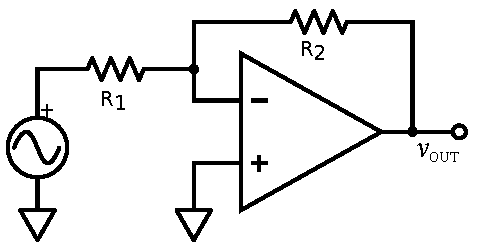
\includegraphics[width=0.28\textwidth]{../E03/latex/HF_ol.pdf}
  \end{center}
  \caption{Circuito utilizzato per stimare il guadagno $A_{ol}$ a basse frequenze. I valori delle resistenze utilizzate sono le stesse del circuito in Figura \ref{cir3:low_frequency}.}
  \label{cir3:high_frequency}
\end{wrapfigure}

Per non dover utilizzare resistenze $R_4$ troppo grandi ad alte frequenze ($>$ \SI{70}{\kilo\hertz}), abbiamo provato ad effettuare le misure direttamente ad open-loop, dato che il guadagno è contenuto (\num{<100}).
Tuttavia il generatore di forme d'onda non emette un segnale pulito alla sola frequenza voluta, in quanto anch'esso è uno strumento reale e dunque affetto da errori.
Esso potrebbe dunque emettere segnali a frequenze basse o addirittura un piccolo offset.
Poichè per tali frequenze il guadagno dell'amplificatore operazionale è enorme, il segnale in uscita viene immediatamente distorto da tali rumori indesiderati.
Non è da sottovalutare poi la presenza dei residui dell'offset dell'opamp.
Esso infatti dipende anche dalla temperatura e dunque la sua compensazione non potrà mai essere perfetta ad ogni temperatura.
Misurare il guadagno $A_{ol}$ effettivamente a open-loop è particolarmente problematico.

Per aggirare tali ostacoli possiamo utilizzare il circuito riportato in Figura \ref{cir3:low_frequency}, rimuovendo la resistenza $R_4$ e sostituendo $R_3$ con un filo partendo dalla configurazione di Figura \ref{cir3:high_frequency}.
Cosi facendo otteniamo la semplice relazione $A_{ol}=\frac{{V_{out}}^{pp}}{{V_A}^{pp}}$, che possiamo anche vedere come limite di eq. (\ref{eq3:lfgain}) per $R_4 \rightarrow \infty$.
I dati ottenuti sono riportati nel seguente grafico. 

\begin{figure}[h]
	\centering
	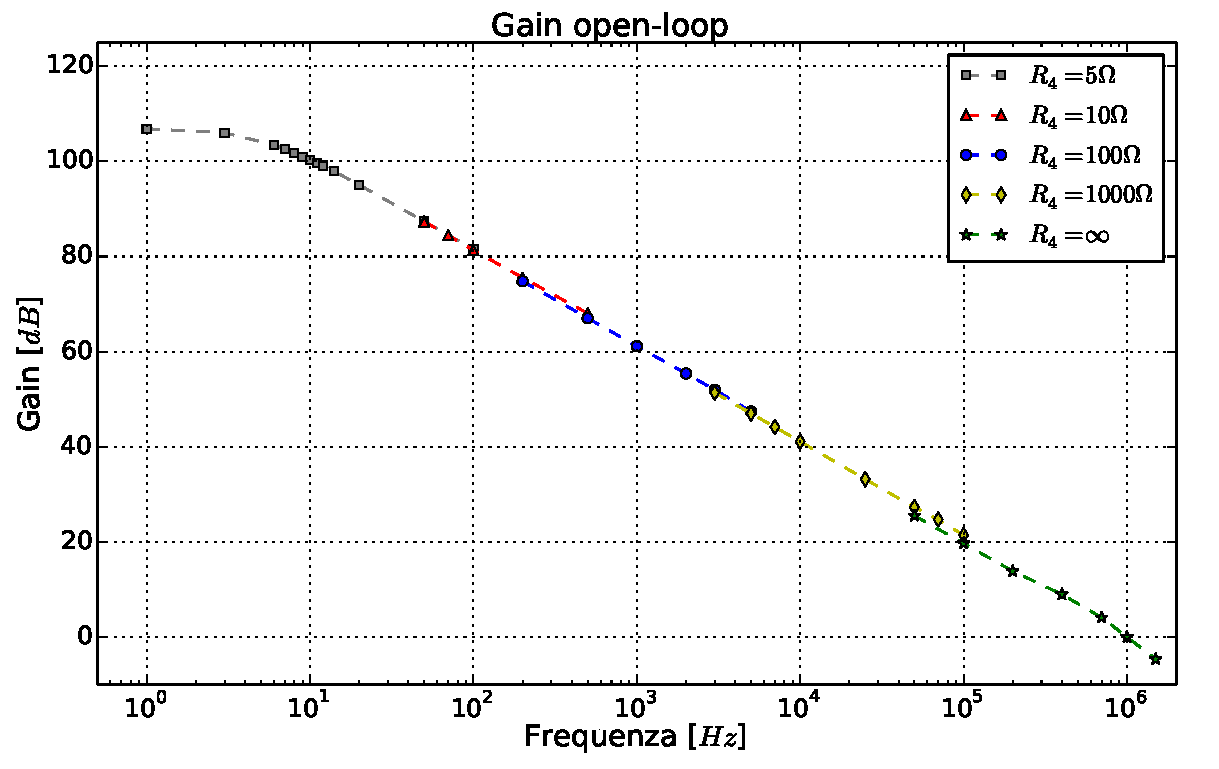
\includegraphics[width=0.9\textwidth]{../E03/latex/gol.pdf}
	\caption{Grafico semilogaritmico del guadagno (in $dB$) in funzione della frequenza. Ad ogni forma dei punti (e relativo colore) corrisponde una diversa resistenza $R_4$ utilizzata. Per quanto riguarda $R_4=\infty$, intendiamo la mancanza del collegamento fra ingresso invertente e non invertente (circuito in Figura \ref{cir3:high_frequency}). La legge plottata è la (\ref{eq3:fit_gain_ol}).}
  \label{cir3:gain_open_loop}
\end{figure}

Anche in questo caso, considerando l'operazionale come un semplice passa basso, possiamo utilizzare l'equazione (\ref{eq3:passa_basso}) e trovare la relazione fra il guadagno e la frequenza. Otteniamo
\begin{equation}
\mathrm{Gain}=\frac{|V_{out}|}{|V_{in}|}=\frac{A_{ol} \omega_0}{\sqrt{\omega^2 + \omega_0^2}}
\label{eq3:fit_gain_ol}
\end{equation}


\subsection{Calcolo di $A_{ol}$}
\label{par3:A_ol}

\subsubsection{$A_{ol}$ da circuiti retroazionati}

Con un fit sulle leggi (\ref{eq3:fit_gain}) e (\ref{eq3:fit_fase}) abbiamo ottenuto una stima dei parametri di $A_{ol}$ e $\omega_0$. Abbiamo deciso, dato che l'opamp utilizzato era lo stesso per tutte le misurazioni, di procedere con una media pesata sui valori ottenuti con i 4 fit (due con (\ref{eq3:fit_gain}) e due con (\ref{eq3:fit_fase})), ottenendo i seguenti valori sperimentali
$$A_{ol}=(1.8\pm0.1)\times 10^5 \qquad f_0=(5.9\pm0.2)\si{\hertz}$$

Ovviamente possiamo ottenere un valore di $A_{ol}$ anche utilizzando la (\ref{eq3:freq_taglio})
$$A_{ol} = \frac{G}{\omega_0} (\omega_t - \omega_0)$$
e considerando la frequenza $f_0$ ricavata dal fit. Si ottiene un valore teorico (media dei valori con i due guadagni del circuito) di $A_{ol} = (1.71\pm 0.06)\times 10^5$, compatibile con il valore sperimentale.

\subsubsection{$A_{ol}$ da open loop}

Con il fit dalla (\ref{eq3:fit_gain_ol}) otteniamo i seguenti valori
$$A_{ol}=(2.0\pm0.1)\times 10^5 \qquad f_0=(5.8\pm0.2)\si{\hertz}$$

Confrontando i risultati ottenuti con i 2 fit vediamo subito che sono compatibili tra loro. 

\subsection*{Conclusioni}

In questa esperienza siamo riusciti a stimare lo "slew rate" di un amplificatore operazionale $\mu$A741 e la massima corrente erogata. Tali valori sono risultati compatibili con quelli riportati sul datasheet del costruttore. 

Successivamente abbiamo verificato la banda passante per un circuito non invertente retroazionato negativamente con guadagno G=11 e G=101. Dai diagrammi di Bode abbiamo visto come aumentando il Gain diminuiva la banda passante (ovvero GBWP=const).

Infine abbiamo valutato il guadagno open-loop a diverse frequenze, utilizzando dei circuiti che ci permettevano un controllo del guadagno effettivo e dunque di evitare problemi quali la saturazione dell'amplificatore operazionale. Il guadagno open-loop per tensioni costanti è stato stimato essere un valore compreso fra \num{1.8E5} e \num{2.0E5}, valore compatibile con quelli forniti dal costruttore.


\newpage

\setcounter{footnote}{0}

\section{08.10.2014 - Comparatori}

In questa esperienza studieremo dei circuiti comparatori con retroazione positiva. In particolare, analizzeremo il funzionamento del \textit{trigger di Schmitt} non invertente, dell'oscillatore a rilassamento e di un interruttore crepuscolare.

\subsection*{Strumenti e materiali}

\begin{itemize} [noitemsep]
\item Oscilloscopio Agilent DSO-X 2002A (bandwidth \SI{70}{\mega\hertz}, sample rate \num{2} GSa/s);
\item Generatore di tensione continua Agilent E3631A (max $\pm \, \SI{25}{\volt}$ o $\pm \, \SI{6}{\volt}$);
\item Generatore di forme d'onta Agilent 33120A con range di frequenza da \SI{100}{\micro\hertz} a \SI{15}{\mega\hertz};
\item Multimetro Agilent 34410A a sei cifre e mezza;
\item Un amplificatore operazionale $\mu$A741;
\item Un amplificatore operazionale LM311;
\item Foto-transistor OP550;
\item Resistenze e capacità di vari valori;
\item Un trimmer a un giro da \SI{5}{\kilo\ohm} e uno da \SI{10}{\kilo\ohm};
\item Un trimmer multi-giro da \SI{10}{\kilo\ohm};
\item Breadboard e cablaggi vari.
\end{itemize}

\subsection{Verifica del funzionamento di un comparatore}

\begin{wrapfigure}[18]{r}{0.4\textwidth}
  \begin{center}
    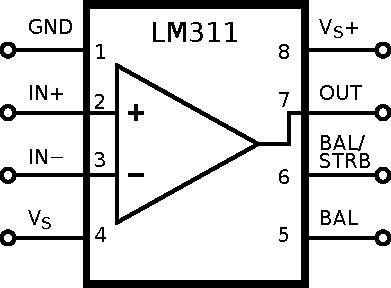
\includegraphics[width=0.280\textwidth]{../E04/latex/LM311.pdf}
  \end{center}
  \caption{Piedinatura dell'operazionale LM311.}
  \label{cir4:piedinatura_LM311}
\end{wrapfigure}

In questa prima parte dell'esperienza abbiamo verificato il funzionamento di un amplificatore operazionale LM311 come comparatore.

Questo amplificatore ha uno slew rate molto alto e lavora sull'ordine dei nanosecondi: rispetto agli $0.5$\si{\volt\per\micro\second} del $\mu$A741, lo slew rate particolarmente elevato permette di confrontare più velocemente i segnali.
Il funzionamento di questo integrato può essere semplificato schematizzandone il funzionamento con un transistor BJT a collettore aperto come in Figura \ref{cir4:open_collector}.
Se colleghiamo anche una resistenza $R$ fra una tensione arbitraria $V_C$, la funzione di output dell'operazionale diventa (se consideriamo il comparatore in configurazione non invertente)

\begin{equation}
V_{out} = \bigg \{
\begin{array}{rl}
V_C & \mathrm{se} \quad V_+ > V_- \\
0 & \mathrm{se} \quad V_+ < V_- \\
\end{array}
\label{eq4:comparatore}
\end{equation}

dove $V_+$ e $V_-$ sono rispettivamente le tensioni all'ingresso non invertente ed invertente. Utilizzando la schematizzazione con il transistor, è come considerare la condizione di quest'ultimo nella seguente maniera

\begin{equation}
Q : \bigg \{
\begin{array}{rl}
\mathrm{interdizione} & \mathrm{se} \quad V_+ > V_- \\
\mathrm{saturazione} & \mathrm{se} \quad V_+ < V_- \\
\end{array}
\label{eq4:comparatore_Q}
\end{equation}

da cui è facile mostrare che la tensione di uscita è proprio (\ref{eq4:comparatore}).

\begin{wrapfigure}[16]{l}{0.5\textwidth}
  \begin{center}
    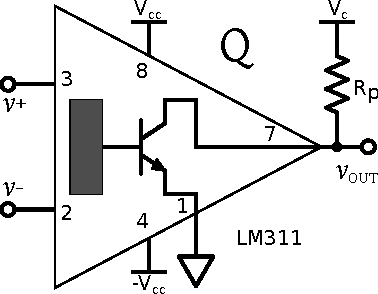
\includegraphics[width=0.280\textwidth]{../E04/latex/c_LM311.pdf}
  \end{center}
  \caption{Schema a collettore aperto dell'amplificatore operazionale LM311.}
  \label{cir4:open_collector}
\end{wrapfigure}

Infatti, quando Q è interdetto il generatore di tensione che fornisce $V_C$ non eroga corrente (l'impedenza dell'oscilloscopio è \SI{1}{\Mohm} e il collegamento con la comune del transistor è interdetto) e non c'è caduta ai capi di $R_p$, dunque $V_{out}=V_C$; quando Q è in saturazione la tensione di uscita (tensione di collettore) si porta circa alla tensione di emettitore, dunque a zero\footnote{In realtà la tensione di uscita risulterà qualche centinaio di \si{\milli\volt} sopra lo $0$. Tale tensione serve a polarizzare il transistor affinché vada in saturazione oltre, ovviamente, alle cadute nelle altre parti della circuiteria interna dell'amplificatore.}. Si noti che la tensione di uscita può essere controllata solo grazie alla presenza della resistenza $R_p$ (definita \textit{resistenza di pull-up}).

Sfruttando questa funzione possiamo dunque confrontare la tensione in entrata su un ingresso con quella all'altro ingresso. Ad esempio, poniamo l'ingresso invertente ad una tensione di soglia $V_{ref}=0$: se vale la (\ref{eq4:comparatore}), ponendo un segnale in alternata sull'ingresso non invertente, l'operazionale restituirà una $V_{out}$ nulla se $V_{in}<V_{ref}$, altrimenti $V_C$. Valutiamo dunque il funzionamento del circuito ipotizzato, il cui schema circuitale è in Figura \ref{cir4:comparatore}, ponendo $V_{C}=5$\si{\volt}. Il grafico in Figura \ref{gr4:comparatore} mostra la tensione in entrata e in uscita.

\begin{figure}[ht]
 \centering
   {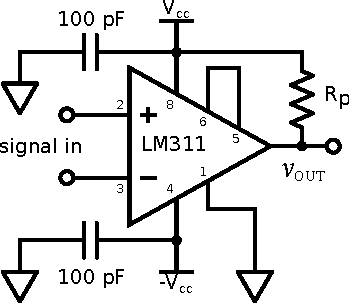
\includegraphics[width=5.5cm]{../E04/latex/c_comparatore.pdf}}
 \caption{Schema completo del comparatore utilizzato. La resistenza $R_p=(9.98 \pm 0.01)$ \si{\kilo\ohm}, come consigliato sul datasheet.}
 \label{cir4:comparatore}
\end{figure}

\begin{figure}[ht]
 \centering
   {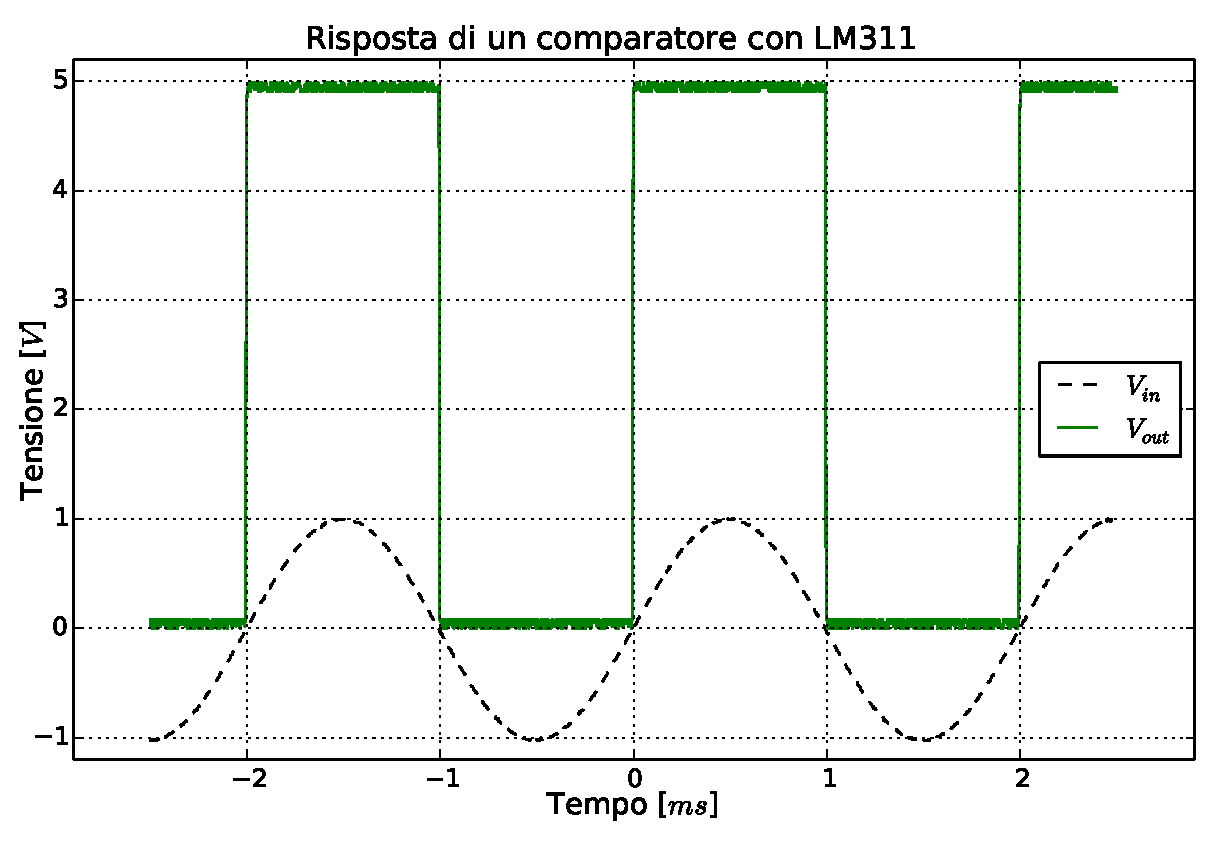
\includegraphics[width=14.5cm]{../E04/latex/comp.pdf}}
 \caption{Grafico della tensione in entrata (onda sinusoidale con $V_{pp}=2$ \si{\volt} e $f=500$\si{\hertz}, tratteggiata) e in uscita (verde) in funzione del tempo. Notiamo che l'uscita rispetta (\ref{eq4:comparatore}).}
 \label{gr4:comparatore}
\end{figure}

\subsection{Trigger di Schmitt non-invertente}

\begin{wrapfigure}[16]{r}{0.50\textwidth}
  \begin{center}
    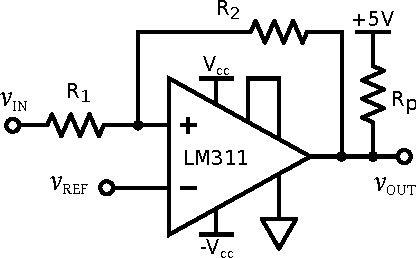
\includegraphics[width=0.320\textwidth]{../E04/latex/c_schmitt.pdf}
  \end{center}
  \caption{Schema del trigger di Schmitt. Le resistenze $R_1$ e $R_2$ sono state variate, mentre $R_p=(9.98 \pm 0.01)$ \si{\kilo\ohm}, come consigliato sul datasheet.}
  \label{cir4:schmitt}
\end{wrapfigure}

Quando nel segnale è presente un rumore è possibile che il valore di tensione restituito dal comparatore cambi più volte da $0$ a $V_{C}$.
Infatti, l'ampiezza in tensione del rumore può essere tale da passare sopra e sotto la tensione di soglia, invertendo la $V_{out}$ più volte, in accordo con (\ref{eq4:comparatore}).

Per ovviare a questo problema si sfrutta la retroazione positiva dell'amplificatore operazionale per riportare parte della $V_{out}$ sull'ingresso non invertente: ciò permette di creare un offset positivo sulla tensione all'ingresso non invertente quando $V_{in}>0$ e viceversa.
Quindi, durante il confronto con la tensione di riferimento, il segnale in entrata risulterà aumentato o diminuito di una certa quantità a seconda di $V_{out}$.

Valutiamo queste tensioni di soglia nel trigger di Schmitt non invertente (grafico in Figura \ref{cir4:schmitt}).
Per fare ciò cerchiamo la dipendenza di $V_{in}$ da $V_{out}$ e da $V^+$ (tensione all'ingresso non invertente). Utilizzando la legge di Kirchhoff sul nodo dell'ingresso non invertente
$$\frac{V_{in}-V^+}{R_1} + \frac{V_{out}-V^+}{R_2} = 0$$
da cui otteniamo
\begin{equation}
V_{in} = V^+ \frac{R_1+R_2}{R_2} - V_{out} \frac{R_1}{R_2}
\label{eq4:v_in_parte2}
\end{equation}
Otteniamo i valori di soglia (che sono valori di $V_{in}$) ponendo la tensione $V^+=V^-=V_{ref}=0$, cioè il punto di tensione di inversione del comportamento del LM311 a collettore comune, e considerando i due valori possibili di $V_{out}$ dati dalla (\ref{eq4:comparatore}), cioè $V_{out}^{inf}=0$ e $V_{out}^{sup}=V_{C}=5$\si{\volt}:
\begin{equation}
V_{soglia}^{sup} = - V_{out}^{inf} \frac{R_1}{R_2} = 0 \qquad V_{soglia}^{inf} = - V_{out}^{sup} \frac{R_1}{R_2} = - (0.46 \pm 0.01) \si{\volt}
\label{eq4:punti}
\end{equation}
da cui è possibile definire la tensione di \textit{isteresi} (cioè la tensione massima in cui un segnale può oscillare attorno alla tensione di riferimento prima di ribaltare l'output del LM311)
$$V_{isteresi} = |\Delta V| = |V_{soglia}^{sup} - V_{soglia}^{inf}| = V_{out}^{sup} \frac{R_1}{R_2} = (0.46 \pm 0.01) \si{\volt}$$

Bisogna tener presente che, come già anticipato, i valori calcolati sono quelli che effettivamente deve raggiungere la $V_{in}$ nel riferimento del generatore di forme d'onda per invertire l'uscita dell'operazionale: infatti non è la tensione di riferimento a cambiare (rimane a comune come si vede nel circuito) come potrebbe succedere in una configurazione invertente, ma il segnale stesso ad essere "alzato" di una tensione data dai valori calcolati. Nel nostro caso, il segnale viene "alzato" di $-V_{inf}^{soglia}>0$ una volta che $V_{in}$ raggiunge $V_{ref}=0$: per cambiare nuovamente l'uscita (porla a 0) sarà il segnale "alzato" a dovere la tensione di riferimento, dunque nel riferimento del generatore di forme d'onda la tensione di inversione sarà negativa e uguale a $V_{inf}^{soglia}<0$.

I punti ottenuti in \ref{eq4:punti} sono visibili nel grafico di isteresi in Figura \ref{gr4:isteresi}.

\begin{figure}[ht]
 \centering
   {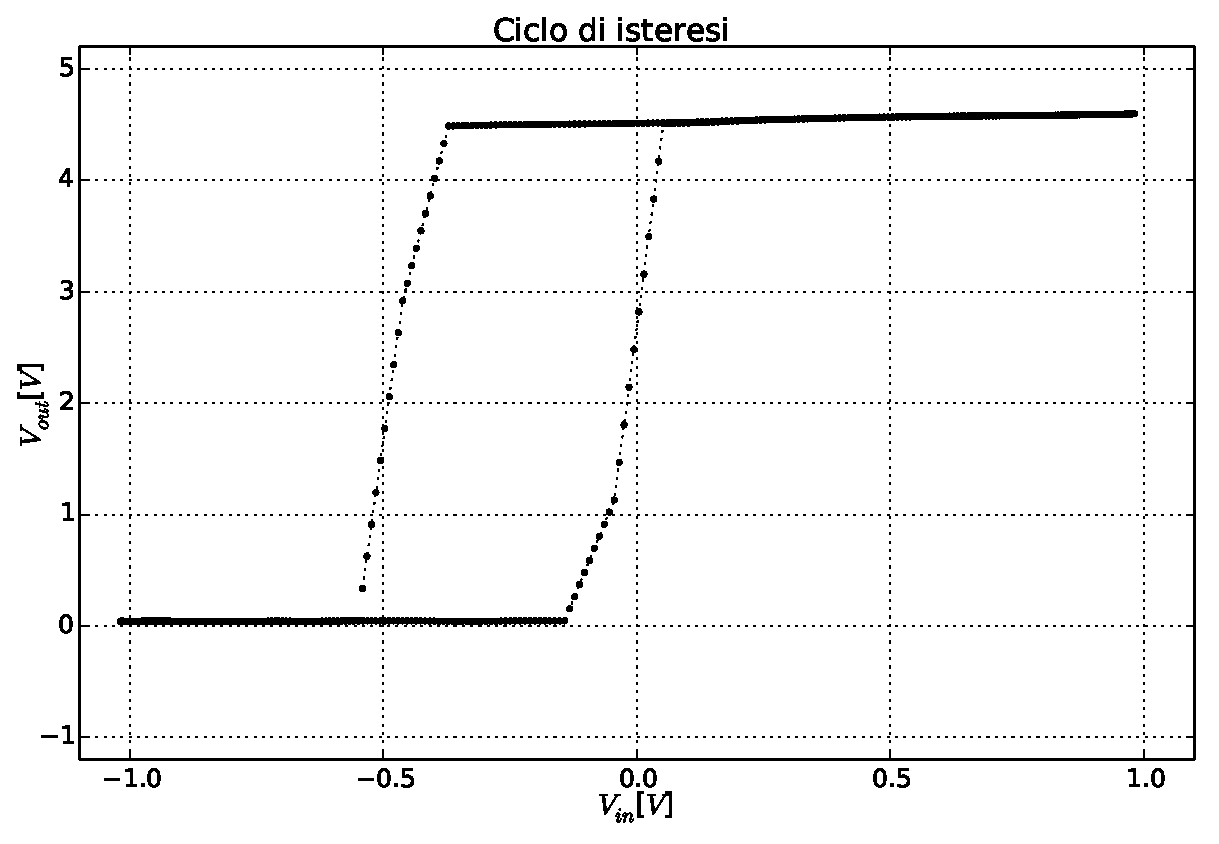
\includegraphics[width=14.5cm]{../E04/latex/XY.pdf}}
 \caption{Grafico dell'isteresi. Per questi dati le resistenze utilizzate sono $R_1=\SI{9.98(1)}{\kohm}$ e $R_2=\SI{99.6(1)}{\kohm}$. Le varie differenze rispetto al grafico ideale sono spiegate nel paragrafo.}
 \label{gr4:isteresi}
\end{figure}

Notiamo però che vi sono alcune incongruenze rispetto al grafico ideale di isteresi: le rette $V_{in}=V_{soglia}$ (per entrambe le soglie) in realtà non sono perpendicolari alle ascisse, e abbiamo ipotizzato che tale comportamento sia imputabile all'entrata dell'opamp in regione lineare, uscendo dalla saturazione.
Inoltre la tensione di uscita massima non è $5$ \si{\volt} perché, a differenza del comparatore in Figura \ref{cir4:comparatore}, la corrente quando Q è interdetto può passare attraverso il circuito di retroazione, provocando una caduta di potenziale sulla resistenza $R$.
Tale corrente dipende inoltre dalla tensione in entrata, dunque è spiegata la pendenza della retta $V_{out}^{sup}$.

Abbiamo infine provato ad inserire un offset all'ingresso invertente: ciò ha portato, come ci aspettavamo dalla relazione (\ref{eq4:v_in_parte2}) (si ricorda che $V^+=V_{ref}$), ad una traslazione del grafico in Figura \ref{gr4:isteresi} di un valore dato dall'offset impostato. Infine, durante l'esperienza, abbiamo anche variato $R_1$ per valutare diverse tensioni di isteresi.

\subsection{Oscillatore a rilassamento}

\begin{wrapfigure}[16]{r}{0.45\textwidth}
  \begin{center}
    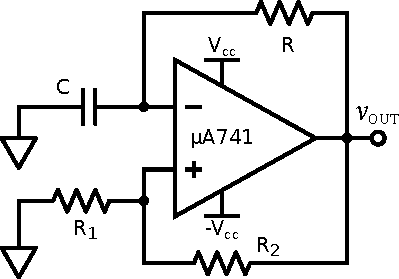
\includegraphics[width=0.30\textwidth]{../E04/latex/c_rilassamento.pdf}
  \end{center}
  \caption{Schema completo dell'oscillatore a rilassamento.}
  \label{cir4:oscillatore}
\end{wrapfigure}

In questa parte dell'esperienza studieremo il funzionamento di un oscillatore a rilassamento. Tale circuito sfrutta l'instabilità della retroazione positiva per generare un segnale oscillante con una frequenza determinata dai componenti stessi del circuito. In Figura \ref{cir4:oscillatore} è riportato lo schema circuitale. 

L'elemento circuitale fondamentale per il funzionamento dell'oscillatore a rilassamento è il condensatore C.  Sfruttando il trigger di Schmitt dato dalle resistenze $R_1$ ed $R_2$, la tensione di riferimento (cioè la tensione $V_+$ all'ingresso non invertente) cambia al cambiare di $V_{out}$ come segue
$$
V_{+} = \bigg \{
\begin{array}{rl}
\beta V_{cc} & \mathrm{se} \quad V_+ > V_- \quad \mathrm{ovvero} \quad V_{out}=V_{cc}\\
-\beta V_{cc} & \mathrm{se} \quad V_+ < V_- \quad \mathrm{ovvero} \quad V_{out}=-V_{cc}\\
\end{array}
$$
dove $\beta=\frac{R_1}{R_1+R_2}$ è dato dal partitore fra $R_1$ ed $R_2$.
Nel nostro caso, la capacità renderà la tensione $V_-$ all'ingresso invertente crescente (verso $V_{cc}$) quando $V_{out}=V_{cc}$ e decrescente nel caso opposto. Inoltre, $V_-$ invertirà il segno della derivata una volta raggiunta la tensione $\pm \beta V_{cc}$.

Infatti, supponiamo ad esempio che la tensione $V_-$ stia crescendo. Ciò significa, per quanto detto, che la tensione di riferimento è data dal trigger, cioè $V_+=\beta V_{cc}$. Dunque, una volta raggiunta e superata tale tensione il confronto fra le due invertirà la tensione di uscita e $V_-$ inizierà a decrescere fino a $-\beta V_{cc}$, per poi invertirsi di nuovo. Tale processo porta quindi ad una oscillazione a rilassamento, cioè verso una stabilizzazione a $\pm V_{cc}$ che però non può avvenire per la presenza del trigger. Il periodo di tale oscillazione può essere calcolato risolvendo il circuito.
%Per comodità a $t=0$ assumiamolo scarico e $V_{out}=+V_{sat}$. Ovviamente, per effetto della retroazione negativa, la tensione all'ingresso invertente tenderà ad aumentare ($V_{inv}$ è determinata da quanta carica è accumulata sul condensatore). Non appena $|V_{inv}|>|V_{ninv}|$, avremo uno switch della tensione in uscita, ovvero $+V_{sat} \rightarrow -V_{sat}$. Il condensatore inizierà dunque a scaricarsi. Successivamente avremo un altro switch della tensione in uscita e il ciclo si ripeterà. Il periodo di tale oscillazione può essere calcolato risolvendo il circuito.

A tal fine consideriamo la parte del circuito costituita dalla capacità C e dalla resistenza R per valutarne la risposta al gradino (cioè quando la tensione in uscita dal $\mu$741 passa da $-V_{cc}$ a $V_{cc}$), schematizzandolo come in Figura \ref{cir4:oscillatore_spi}, in quanto è il comportamento della capacità che ci interessa per il calcolo del periodo $T$.

\begin{wrapfigure}[23]{l}{0.28\textwidth}
  \begin{center}
    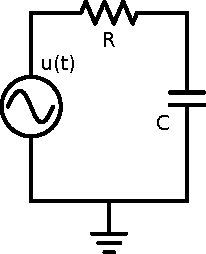
\includegraphics[width=0.26\textwidth]{../E04/latex/c_rilassamento_spi.pdf}
  \end{center}
  \caption{}
  \label{cir4:oscillatore_spi}
\end{wrapfigure}

Per la legge di Kirchhoff sulle correnti vale
$$\frac{u(t)V_{cc} - V(t)}{R} - C \frac{dV(t)}{dt} = 0$$
con $u(t)=1$ per $t>0$ e $V(t)=V_-$ la differenza di potenziale del condensatore. Quindi otteniamo
$$\frac{1}{V_{cc} - V(t)} \frac{dV(t)}{dt} = \frac{1}{RC}$$
L'equazione differenziale ha come soluzione
$$V(t)=V_{cc} - a e^{-\frac{t}{RC}}$$
Per trovare la costante $a$ dobbiamo considerare il grafico in Figura \ref{gr4:osc10k} e impostare $V(t=0)=-\beta V_{cc}$. Quindi si ricava che
\begin{equation}
V(t)=V_{cc} - V_{cc} (1+ \beta) e^{-\frac{t}{RC}}
\label{eq4:osc_vt}
\end{equation}
Sempre dal grafico sperimentale in Figura \ref{gr4:osc10k} è possibile imporre che $V(T/2)=\beta V_{cc}$. Imponendo l'uguaglianza di questa condizione con (\ref{eq4:osc_vt}) e svolgendo i calcoli il valore che si ottiene per il periodo è
\begin{equation}
T=2RCln\left(1+\frac{2R_1}{R_2}\right)
\label{eq4:periodo_osc}
\end{equation}  

Nel grafico in Figura \ref{gr4:osc10k} sono riportati i risultati ottenuti per valori di $R=\SI{9.99(1)}{\kohm}$. Come vediamo, carica e scarica del condensatore tendono a $\pm V_{sat}$.

Nella seguente tabella riportiamo i valori del periodo teorici calcolati con (\ref{eq4:periodo_osc}), e sperimentali. Osserviamo che i due valori sono compatibili.

\begin{center}
{\renewcommand{\arraystretch}{1.2}%
	\begin{tabular}{c|c|c}
    %\hline
	$R$ [\si{\kilo\ohm}] & $T_{exp}$ [\si{\milli\second}] & $T_{teo}$ [\si{\milli\second}]\\
    \hline
	$9.99\pm0.01 $ & $2.22\pm0.01$ & $2.19 \pm 0.03$\\
    \hline
	$99.93\pm0.01 $ & $22.2\pm0.1$ & $21.9 \pm 0.3$\\
    %\hline
	\end{tabular}
}
\end{center}

\begin{figure}[ht]
 \centering
   {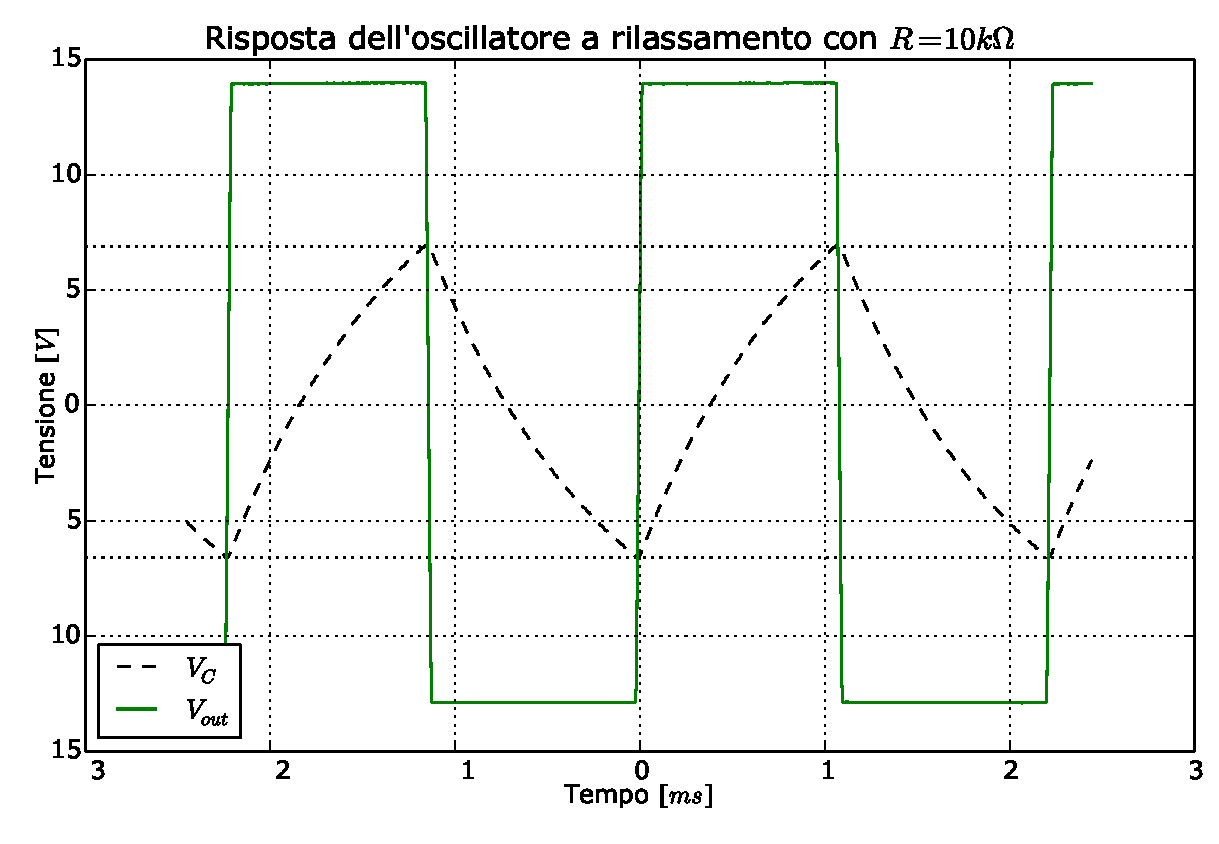
\includegraphics[width=14.5cm]{../E04/latex/osc10k.pdf}}
 \caption{Tensione di output del circuito oscillatore a rilassamento in funzione del tempo. I valori degli elementi circuitali sono: $C=\SI{85.0(5)}{\nano\farad}$, $R=\SI{9.99(1)}{\kohm}$, $R_2= \SI{9.96(1)}{\kohm}$ e $R_2=\SI{9.98(1)}{\kohm}$.}
 \label{gr4:osc10k}
\end{figure}

\subsection{Interruttore crepuscolare}

Nell'ultima parte dell'esperienza abbiamo assemblato un interruttore crepuscolare, cioè un circuito elettronico che alimenta un carico (LED) in condizioni di bassa luminosità ambientale e interrompe l'alimentazione in condizioni di alta luminosità ambientale.

\begin{figure}[ht]
 \centering
   {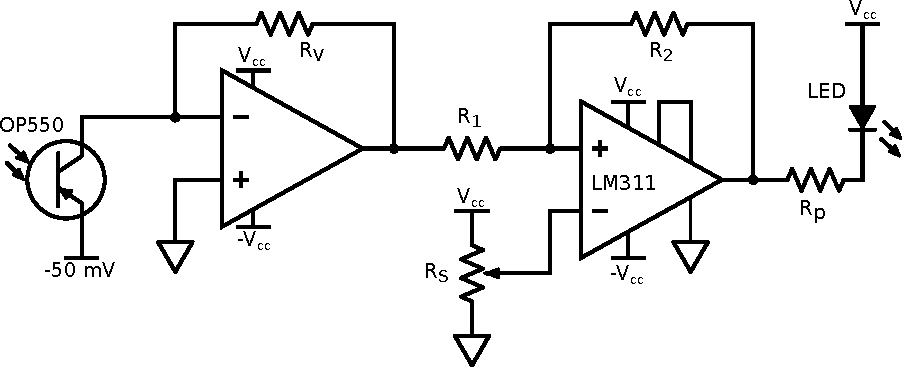
\includegraphics[width=12.5cm]{../E04/latex/c_crepuscolare.pdf}}
 \caption{Circuito dell'interruttore crepuscolare. Come vediamo chiaramente, la parte con l'opamp $\mu$A741 è un semplice amplificatore in tensione ($R_F = \SI{1}{\Mohm}$) La seconda parte del circuito è un comparatore con isteresi, settata dal rapporto $R_1/R_2$ ($R_1 = \SI{50}{\kohm}$ e $R_2 = \SI{100}{\kohm}$). La tensione di riferimento deve essere scelta in modo da decidere con quanta luminosità si vuole che l'interruttore scatti. Per far ciò abbiamo usato un partitore utilizzando un trimmer ($R_S$) da \SI{10}{\kohm}. La resistenza di pull-up è stata scelta di  \SI{1}{\kohm}, così da avere una corrente sufficiente per far accendere il led.}
 \label{cir4:crepuscolare}
\end{figure}

Un circuito di questo tipo necessità di almeno due componenti: il sensore di luminosità (foto-transistor OP550) che fornisce la variabile circuitale collegata alla luminosità ambientale e un blocco di comparazione che \textit{decide} se alimentare o meno il carico confrontando il segnale dato dal primo blocco con un segnale di riferimento.

Il componente principale del primo blocco è il foto-transistor OP550 che agisce come una sorgente di corrente, generando una corrente dell'ordine del \si{\uA} se esposto alla luce.
Tale corrente è però difficilmente manipolabile, pertanto abbiamo deciso di utilizzare un convertitore corrente-tensione per trasformare e amplificare il segnale in modo tale da poter essere utilizzata come segnale di ingresso del secondo blocco.

\begin{figure}[ht]
 \centering
   {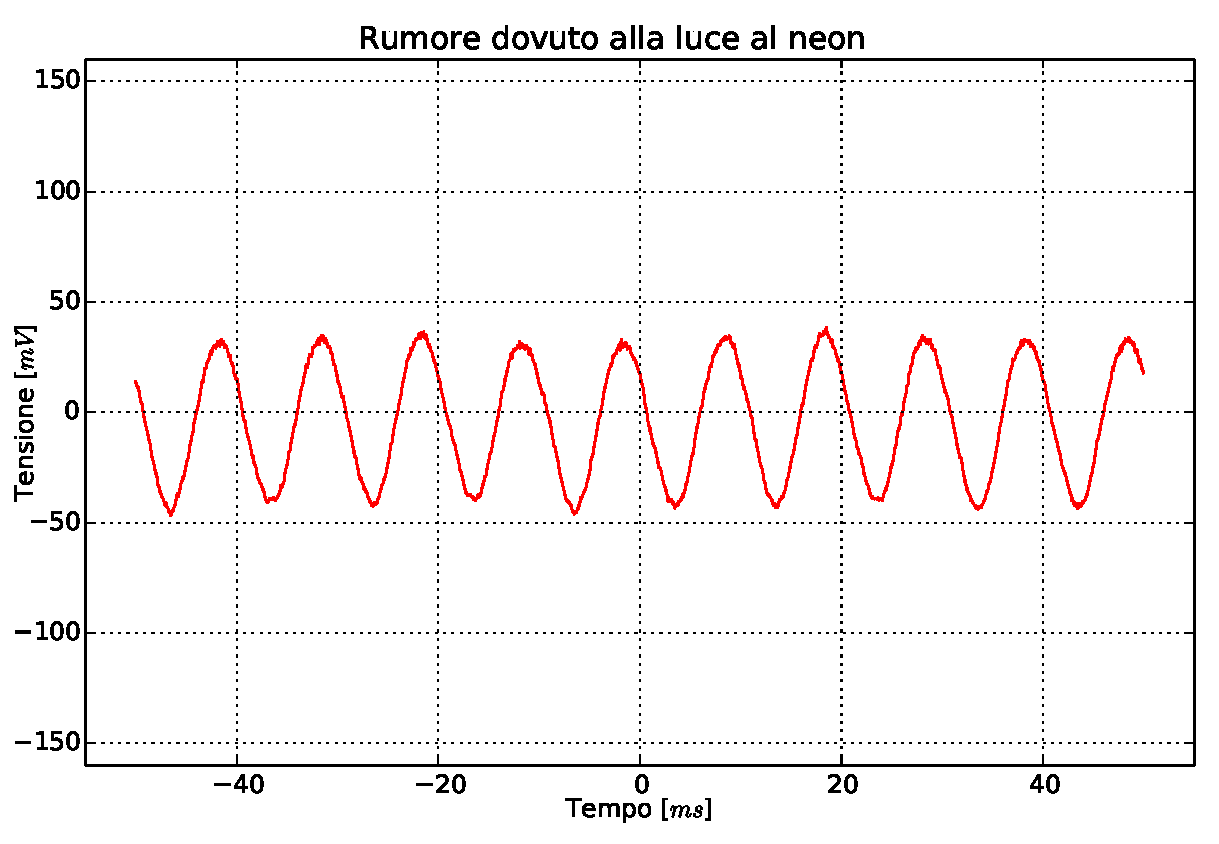
\includegraphics[width=14.5cm]{../E04/latex/neon.pdf}}
 \caption{Rumore ambientale determinato dalla luce delle lampade al neon del laboratorio incidente sul foto-transistor e amplificato dall'opamp $\mu$A741. I dati sono stati ricavati separando i due blocchi del circuito e misurando la tensione all'uscita dell'opamp $\mu$A741.}
 \label{gr4:neon}
\end{figure}

Un convertitore corrente-tensione può essere implementato facilmente utilizzando un opamp $\mu$A741 in modalità di amplificatore invertente con retroazione negativa (vedi Figura \ref{cir4:crepuscolare}).
In questo modo, la tensione in uscita dell'opamp sarà legata alla corrente che attraversa il sensore dalla seguente equazione:

\begin{equation}
	V_{out} = R_F \,\, I_{OP550}
\end{equation}
dove $R_F$ è la resistenza posta sul ramo di retroazione (nel nostro caso $R_F = \SI{1}{\Mohm}$) e $I_{OP550}$ è il modulo della corrente passante nel foto-transistor.

Il secondo blocco del circuito è invece composto da un opamp LM311 utilizzato come comparatore con isteresi (o trigger di Schmitt).
Sul ramo di retroazione e tra il terminale positivo e l'ingresso del segnale (che corrisponde all'uscita dell'opamp $\mu$A741) sono state poste due resistenze per creare l'isteresi affinché eventuali rumori di fondo non disturbassero il funzionamento del circuito.
Nel nostro caso abbiamo utilizzato due resistenze $R_1 =$ \SI{5}{\kohm} e $R_2=$ \SI{100}{\kohm} in modo da avere un ampio margine di sicurezza.

Come si può notare dal grafico in Figura \ref{gr4:neon} il rumore ambientale dato dalle lampade al neon ha una forma d'onda sinusoidale di frequenza \SI{100}{\hertz} e ampiezza picco-picco \SI{80}{\mV}, pertanto sarebbe stata sufficiente una isteresi di appena $\frac{V_{CC}}{100} \approx \SI{150}{\mV}$

Per impostare la tensione di soglia, invece, abbiamo creato un partitore collegando i due connettori esterni di un trimmer resistivo da \SI{10}{\kohm} a +\SI{15}{\V} e a comune, mentre abbiamo collegato il terminale centrale del trimmer all'ingresso invertente del LM311.
In questo modo potevamo scegliere la tensione di soglia girando semplicemente un cacciavite.

Infine abbiamo posto il carico da alimentare tra l'alimentazione positiva +\SI{15}{\V} e la resistenza di pull-up ($R_P=$ \SI{1}{\kohm}).

\subsection*{Conclusioni}

In questa esperienza abbiamo analizzato il funzionamento di circuiti comparatori, molto utili quando vogliamo confrontare due segnali ottenendo un semplice valore digitale (on-off).
Tuttavia, vista la sensibilità degli opamp, abbiamo bisogno di un modo per evitare che il rumore influenzi le nostre comparazioni.
Per far questo abbiamo introdotto i circuiti con isteresi, ovvero con feedback-positivo.

Durante l'esperienza abbiamo anche costruito un oscillatore a rilassamento: la peculiarità di tale circuito è che esso oscilla tra $+V_{sat}$ e $-V_{sat}$ sebbene sia alimentato con tensioni continue.
La frequenza di tale oscillatore è univocamente determinata dai valori delle componenti circuitali.

È stato poi realizzato un interruttore crepuscolare.
Questi interruttori, contenenti un foto-transistor, permettono ad esempio l'accensione (e spegnimento) delle luci stradali quando tramonta il sole.
Non volendo però che una semplice nuvola passeggera faccia accendere le luci, abbiamo introdotto la retroazione positiva per creare una isteresi che renda il circuito insensibile al rumore (la nuvola).

\newpage

\setcounter{footnote}{0}

\section{14.10.2014 - Gruppo Avanzato}

In questa esperienza progetteremo un raddrizzatore di precisione (utilizzabile anche per segnali di bassa tensione). Dopodiché valuteremo la capacità di un amplificatore differenziale e dell'integrato $AD622$ di abbattere i guadagni di modo comune. Infine utilizzeremo una termoresistenza per ricavare la temperatura in alcune situazioni.

\subsection*{Strumenti e materiali}

\begin{itemize} [noitemsep]
\item Oscilloscopio Agilent DSO-X 2002A (bandwidth \SI{70}{\mega\hertz}, sample rate \num{2} GSa/s);
\item Generatore di tensione continua Agilent E3631A (max $\pm \, \SI{25}{\volt}$ o $\pm \, \SI{6}{\volt}$);
\item Generatore di forme d'onta Agilent 33120A con range di frequenza da \SI{100}{\micro\hertz} a \SI{15}{\mega\hertz};
\item Multimetro Agilent 34410A a sei cifre e mezza;
\item Un amplificatore operazionale $\mu$A741;
\item Un integrato AD622;
\item Una termoresistenza PT100;
\item Resistenze e capacità di vari valori;
\item Due trimmer multigiro da \SI{10}{\kilo\ohm};
\item Breadboard e cablaggi vari.
\end{itemize}

\subsection{Raddrizzatore di precisione}

\subsubsection{Premessa sui raddrizzatori}

I raddrizzatori sono dei circuiti il cui scopo è quello di effettuare il modulo di un segnale in ingresso preservandone la forma. In precedenti corsi di optoelettronica abbiamo incontrato alcuni semplici raddrizzatori i cui elementi circuitali chiave erano i diodi. Questi dispositivi sono in grado di portarsi in conduzione, e quindi di chiudere il ramo di circuito in cui si è posto il diodo, se la tensione al polo positivo è maggiore di quella al polo negativo; altrimenti il diodo apre il circuito. In realtà, ciò accade unicamente nel caso in cui il diodo sia ideale: per polarizzare un diodo è infatti necessario creare una differenza di tensione ai suoi capi, detta tensione di soglia $V_d$, che ha un valore di $\approx 0.6$ \si{\volt}; altrimenti il diodo risulterà come non polarizzato e dunque non in conduzione. Questo fatto, nella creazione di raddrizzatori può creare alcuni svantaggi, soprattutto se necessaria un'alta precisione (lavorando con piccoli valori di tensione): il segnale in uscita sarà con la stessa forma d'onda del segnale in entrata, ma con un offset di $-0.6$\si{\volt} dato dalla $V_d$; inoltre, se i segnali in entrata hanno valori più piccoli della tensione di soglia, il diodo non entrerà mai in conduzione. Di seguito presentiamo alcuni circuiti che risolvono in parte queste problematiche.

\subsubsection{Raddrizzatore con un diodo}

Analizziamo il circuito in Figura ?????. Vogliamo dimostrare che, qualunque sia il segnale in entrata, il contributo alla tensione di uscita dato dalla tensione di soglia del diodo è trascurabile.

Innanzitutto notiamo che, dato l'alto guadagno dell'operazionale, la tensione in entrata per polarizzare il diodo è un valore molto basso (con un guadagno di $2\times 10^5$ la tensione necessaria è data da $0.6 \si{\volt}/2\times 10^5 \approx 3 \si{\micro\volt}$); dunque non dobbiamo preoccuparci che il segnale in entrata debba avere un valore minimo per far funzionare il circuito.

Vale per l'operazionale l'equazione (\ref{eq3:regola_opamp})\footnote{In realtà bisognerebbe considerare anche la dipendenza dalla frequenza. Abbiamo però notato che, ben prima che si possa apprezzare l'abbattimento dell'amplificazione, incorreremo in un altro problema dato dalla velocità di polarizzazione dei transistor all'interno dell'operazionale che ci porterà a scartare questo circuito come raddrizzatore di precisione ad alte frequenze.}
\begin{equation}
V_{ol}=A (V^+-V^-)
\label{eq5:regola_opamp_NOFREQDEP}
\end{equation}
dove $V_{ol}$ è la tensione all'uscita dell'amplificatore operazionale.
Valutiamo ora il circuito in due casi: $V_{in}<0 e V_{in}>0$\footnote{Grazie alle considerazioni sopra possiamo trascurare la tensione in ingresso necessaria per polarizzare il diodo}.

\paragraph*{Caso $V_{in}<0$}

Nel primo caso, l'OPAMP amplifica il segnale negativo in entrata sull'uscita rispettando la (\ref{eq5:regola_opamp_NOFREQDEP}) con $V_-=0$: infatti, essendo il diodo interdetto (il polo positivo è più negativo di quello negativo), non passa alcuna corrente per $R_L$ rendendo $V^-=V_{out}=0$.

\paragraph*{Caso $V_{in}>0$}

Nel secondo caso invece il diodo è in conduzione. Consideriamo dunque, come si nota dalla Figura ??????
$$V^+=V_{in} \qquad V^-=V_{out}$$
Dato che un diodo in conduzione ha una caduta in buona approssimazione costante $V_d$, vale anche che
$$V_{ol}=V_{out}+V_d$$
Sostituendo questi risultati in (\ref{eq5:regola_opamp_NOFREQDEP}) otteniamo le equazioni cercate
\begin{equation}
V_{out}=\frac{1}{1+A} (A V_{in} - V_d) \approx V_{in} \qquad V_{ol} \approx V_{in}+V_d
\label{eq5:leggi_1.1}
\end{equation}

Di seguito proponiamo i grafici delle leggi sopra ricavate plottate con i dati sperimentali.

Dal plot del segnale in entrata ed in uscita in funzione del tempo alla frequenza di ?????? \si{\hertz} (grafico in Figura ???????), possiamo notare un troncamento della forma d'onda del segnale in uscita. Abbiamo ipotizzato che tale fenomeno fosse dovuto alla limitata velocità che i transistor all'interno dell'operazionale hanno di passare dalla saturazione all'interdizione; tale fenomeno è anche amplificato dal fatto che, quando il diodo è interdetto, $V_{ol} \approx -V_{CC}$: il segnale deve quindi passare da una tensione di saturazione negativa alla tensione necessaria per raddrizzare il segnale in uscita in un tempo troppo breve, e ad alte frequenze ciò risulta in un troncamento. Per risolvere tale problema utilizziamo il circuito esposto al sottoparagrafo successivo.

\subsubsection{Raddrizzatore con due diodi}

Per risolvere il problema visto in precedenza, utilizziamo un secondo diodo posto come nel in Figura ?????? e un circuito di retroazione controllata in guadagno. Anche in questo caso dobbiamo valutare la risposta del circuito in casi diversi: $V_{in}=0$, $V_{in}>0$ e $V_{in}<0$.

\paragraph*{Caso $V_{in}=0$}

Nel primo caso abbiamo entrambi i diodi interdetti. Infatti, se la tensione in ingresso è nulla non vi è la tensione necessaria a polarizzare i diodi, che rimangono non polarizzati. Dunque $V_{out}=V_{ol}=0$.

\paragraph*{Caso $V_{in}>0$}

Tenendo conto della (\ref{eq5:regola_opamp_NOFREQDEP}), considerando che $V_{in}$ viene portata sull'ingresso invertente, la tensione su $V_{ol}$ sarà negativa e quindi più bassa di $V_{out}$: dunque $D_2$ sarà interdetto. Allo stesso tempo il polo positivo di $D_1$ è più positivo (a comune virtuale) di quello negativo ($V_{ol}$), dunque tale diodo risulta in conduzione. Inoltre, $V_{out}$ risulta nulla in quanto sul ramo di circuito identificato da $R_2$ e $R_L$ non passa corrente (sono collegate rispettivamente a comune virtuale e comune). $V_{ol}$ sarà invece fissata dalla tensione di soglia del diodo, cioè $V_{ol}=-V_d$.

\paragraph*{Caso $V_{in}<0$}

Con considerazioni analoghe al caso precedente, possiamo concludere che $D_1$ risulta interdetto, mentre $D_2$ in conduzione. Quindi il circuito è un amplificatore invertente di segnale con guadagno $-R_2/R_1$.

Valutiamo il contributo del diodo nella tensione di uscita del circuito $V_{out}$ e dell'operazionale $V_{ol}$. Consideriamo le correnti nel nodo $V_N$
$$\frac{V_{in}-V_N}{R_1} + \frac{V_{out}-V_N}{R_2} = 0$$
Osservando che $V_N$ è a ground virtuale, che $V_{out}=V_{ol}-V_d$, e considerando l'operazionale come ideale e che vale che $V_{out}=V_{ol}-V_d$, dalla (\ref{eq5:regola_opamp_NOFREQDEP}) otteniamo
$$V_{out}=-\frac{R_2}{R_1}V_{in} \qquad \frac{R_2}{R_1} V_{in} + V_d$$

Di seguito presentiamo i grafici delle tensioni.

INSERIRE GRAFICI E COMMENTARE!
\subsection{Amplificatore differenziale}

\begin{wrapfigure}[14]{l}{0.5\textwidth}
  \begin{center}
    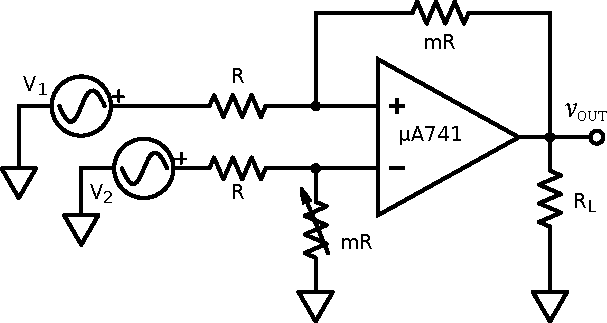
\includegraphics[width=0.33\textwidth]{../E05/latex/c_teo_diff_amp.pdf}
  \end{center}
  \caption{Grafico teorico di un amplificatore differenziale. Per $m$ si intende un fattore moltiplicativo rispetto alla $R$.}
  \label{cir5:diff_amp_teo}
\end{wrapfigure}

In questa parte dell'esperienza cercheremo di capire e analizzare un amplificatore differenziale, il cui schema circuitale è in Figura \ref{cir5:diff_amp}. Oltre al fatto che scegliendo i valori di resistenza possiamo decidere il guadagno, la proprietà più importante è sicuramente l'abbattimento del rumore di modo comune. Per capirne il motivo analizziamo il circuito teorico riportato in Figura \ref{cir5:diff_amp_teo}.

Sfruttiamo il principio di sovrapposizione per valutare la tensione in uscita in funzione delle due di ingresso, ricordandoci che tale principio può essere applicato per sistemi lineari: ciò è molto utile in quanto ci permette di separare l'analisi circuitale e ricondurci a casi più semplici.

Chiamiamo $V^-$ la tensione all'ingresso invertente e $V^+$ quella all'ingresso non invertente. Analizziamo prima il caso in cui $V_1=0$. La tensione nel punto $V_+$ sarà data dal partitore con $R$ ed $mR$ (verso l'op-amp non scorre corrente). Assumendo l'op-amp ideale, abbiamo $V^+=V^-$. Possiamo dunque scrivere:

\begin{equation}
\begin{cases} V_+=V_-  \\ V_+=V_2\frac{mR}{R+mR} \\ V_-= V_{out2}\frac{R}{R+mR}\end{cases}  \Rightarrow V_{out2}=mV_2
\label{eq 5: vout2}
\end{equation}

Analogamente, poniamo $V_2=0$. Otteniamo le seguenti equazioni del circuito:

\begin{equation}
\begin{cases} V_+=V_-=0  \\ \frac{V_1}{R}+\frac{V_{out2}}{mR}=0 \end{cases}  \Rightarrow V_{out1}=-mV_1
\label{eq 5: vout1}
\end{equation}

Sommando ora (\ref{eq 5: vout2}) e (\ref{eq 5: vout2}) otteniamo $V_{out}=m(V_2-V_1)$.

Possiamo ora passare ad analizzare il circuito da cui siamo partiti, ovvero quello affetto da noise (da noi simulato con un'onda sinusoidale) riportato in Figura \ref{cir5:diff_amp}. Valgono dunque le seguenti equazioni

%\begin{center}
$$
\begin{cases} V_1=V_{in}+V_{noise} \\ V_2=V_{noise} \end{cases}  \Rightarrow V_{out}=m(V_{noise}-(V_{in}+V_{noise}))=-V_{in}
$$
%\end{center}

L'amplificatore differenziale ci permette dunque di eliminare in modo efficace il rumore di modo comune. 

Inoltre, abbiamo posto come resistenza collegata tra comune e $V_+$ un trimmer per impostare la tensione di modo comune al più basso valore possibile. Infatti, le resistenze non sono in realtà esattamente uguali e prima di utilizzare il circuito è necessario bilanciarlo in modo da ottenere un segnale il più piccolo possibile quando i segnali in ingresso sono uguali.

\begin{wrapfigure}[17]{r}{0.5\textwidth}
  \begin{center}
    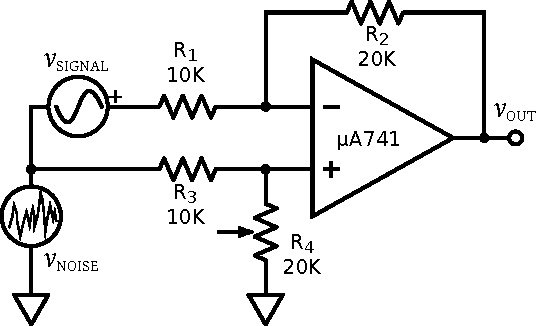
\includegraphics[width=0.33\textwidth]{../E05/latex/c_diff_amp.pdf}
  \end{center}
  \caption{Grafico dell'amplificatore differenziale utilizzato durante l'esperienza. $R_4$ è un trimmer multigiro di resistenza variabile.}
  \label{cir5:diff_amp}
\end{wrapfigure}

In laboratorio abbiamo utilizzato come sorgente di noise il generatore di forme d'onda e come $V_{in}$ il generatore di tensione costante. Abbiamo utilizzato delle R da \SI{10}{\kilo\ohm} e $mR=2R$. La resistenza variabile è stata costruita mettendo in serie una da \SI{10}{\kilo\ohm} con un trimmer, anch'esso da \SI{10}{\kilo\ohm}. Per controllare il bilanciamento abbiamo connesso entrambi gli ingressi al generatore di forme d'onda ed è stato utilizzato un segnale sinusoidale di $20Vpp$. Il segnale in uscita è stato dunque riportato sull'oscilloscopio. Abbiamo notato che, cambiando il valore della resistenza con il trimmer, il segnale in uscita variava. Il miglior bilanciamento che siamo riusciti a raggiungere ha portato la tensione picco-picco del rumore a \SI{0.5}{\milli\volt}. Abbiamo dunque posto come segnale in entrata un valore costante di tensione con il generatore di tensione costante, e alimentato il circuito con $-2Vpp$. Il rumore è sempre stato simulato con una sinusoidale di $20Vpp$. Questo risultato è riportato in Figura \ref{gr5:amp_diff}.

Come vediamo, il rumore è stato completamente eliminato dall'amplificatore differenziale. Abbiamo successivamente provato a sbilanciare il circuito, per vedere l'effetto del rumore sul segnale in uscita. E' stata dunque variata la resistenza con trimmer e abbiamo utilizzato un rumore con dei picchi molto accentuati, così da vedere bene gli effetti sul segnale in uscita (l'output è in Figura \ref{gr5:sbil_amp_diff}). 

\begin{figure}[ht]
 \centering
   {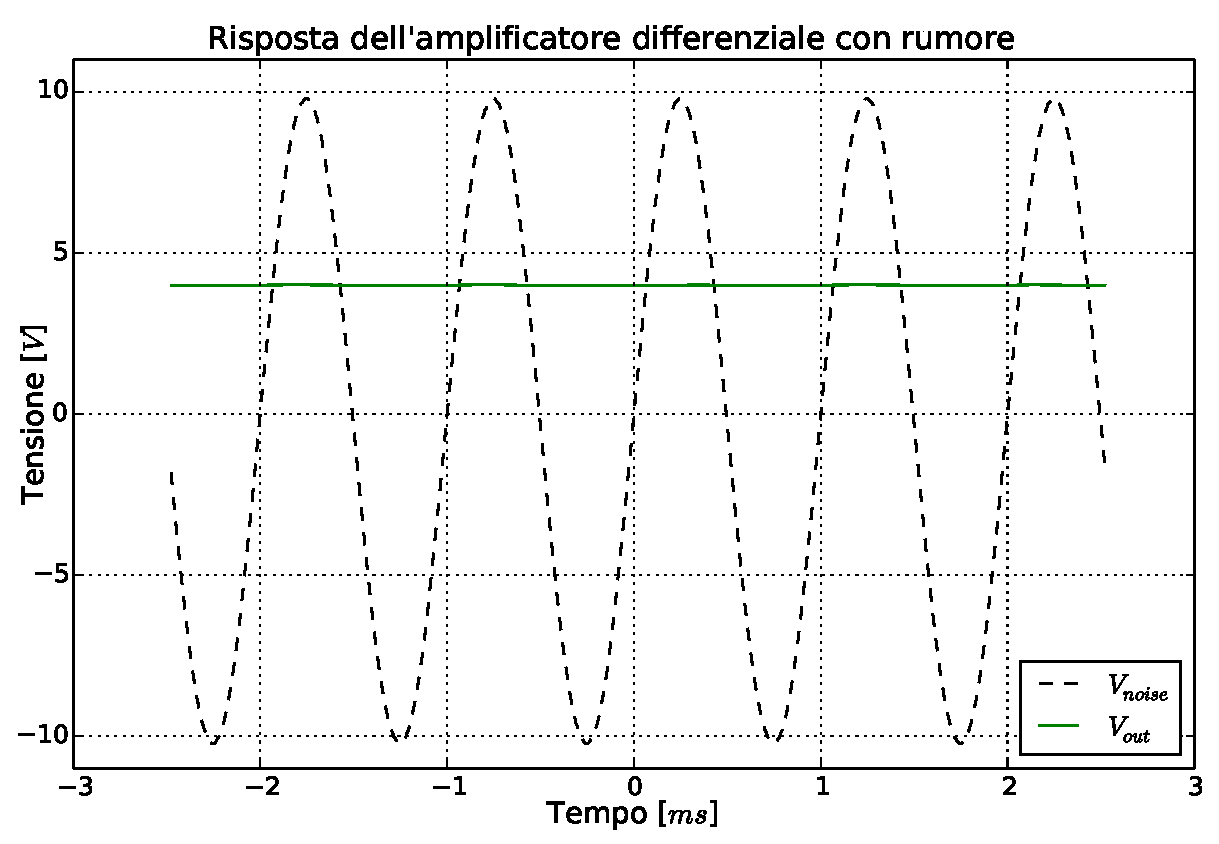
\includegraphics[width=0.85\textwidth]{../E05/latex/amp_diff.pdf}}
 \caption{Come vediamo dal grafico, il rumore che abbiamo simulato ha un'ampiezza di 20 Volt picco-picco (sinusoide in nero). Nonostante ciò, l'uscita (in verde) non è affatto influenzata e risulta amplificata di 2 volte, come stimato precedentemente dai calcoli teorici. }
 \label{gr5:amp_diff}
\end{figure}

\begin{figure}[ht]
 \centering
   {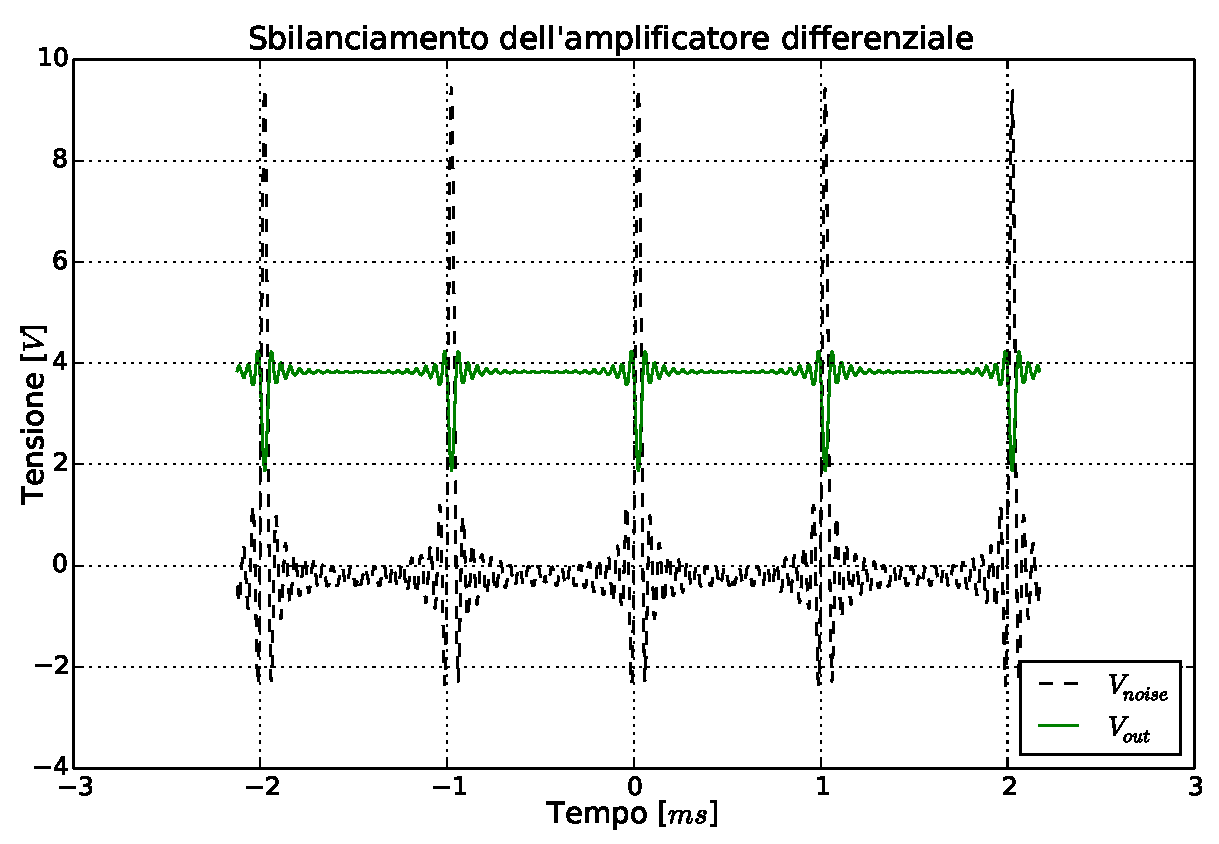
\includegraphics[width=0.85\textwidth]{../E05/latex/sbil_amp_diff.pdf}}
 \caption{Dopo lo sbilanciamento del circuito non è più garantita la soppressione del rumore in modo comune. Come vediamo, il segnale in uscita risulta distorto. E' dunque necessario calibrare bene il circuito prima di effettuare esperimenti nei quali si vuole eliminare un rumore comune ad entrambi i segnali in ingresso.}
 \label{gr5:sbil_amp_diff}
\end{figure}

Inoltre, il guadagno può essere cambiato solo se si cambiano 2 resistenze nel circuito. Una soluzione efficace che inoltre rimedia alla bassa impedenza in ingresso è quella di utilizzare un Amplificatore per Strumentazione, il cui funzionamento è esposto al paragrafo successivo.
\subsection{Instrumentation Amplifier}

\subsubsection{Circuito con Opamp}

\begin{wrapfigure}[17]{r}{0.5\textwidth}
  \begin{center}
    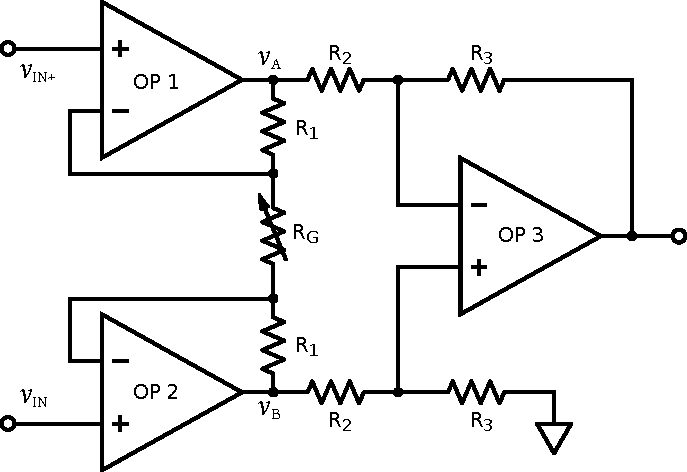
\includegraphics[width=0.350\textwidth]{../E05/latex/c_INA.pdf}
  \end{center}
  \caption{Circuito dell'amplificatore per strumentazione.}
  \label{cir5:instr_amplif}
\end{wrapfigure}

Il circuito visto al paragrafo precedente presenta dei problemi, nonostante abbatta in maniera abbastanza efficiente i segnali di modo comune. Per prima cosa l'impedenza in ingresso vista da un eventuale generatore di segnale è bassa, e ciò rende necessaria una potenza maggiore da parte del generatore per mantenere la tensione ai suoi capi; il secondo luogo, il guadagno non è impostabile (se non cambiando le resistenze ad ogni applicazione: procedura scomoda nelle applicazioni pratiche).

Per ovviare a questi problemi, valutiamo l'amplificatore differenziale in Figura \ref{cir5:instr_amplif}. Si nota subito che l'impedenza in ingresso è molto alta, in quanto gli amplificatori operazionali hanno un valore di impedenza molto alta ai loro ingressi (non a caso sono usati in configurazione follower per adattare le impedenze).

Verifichiamo invece che la resistenza posta in mezzo varia effettivamente il guadagno del circuito. Dividiamo il circuito in due parti, calcolandoci prima la tensione fra il punto A e B\footnote{Si noti che un circuito che abbia come $V_{out}$ la differenza fra questi due punti sarebbe flottante sull'uscita. Infatti, una eventuale resistenza di carico messa fra il punto A e B non avrebbe un riferimento di comune.}, per poi la tensione di uscita dell'intero circuito. Per la prima parte, considerando i due operazionali ideali, otteniamo che le tensione agli ingressi invertenti sono $V_{OP_1}^- = V_1$ e $V_{OP_2}^- = V_2$. Dunque ai capi di $R_g$ è presente una differenza di potenziale $V_2-V_1 = \Delta V_{in}$; per l'idealità degli OPAMP, abbiamo inoltre che la corrente che passa per le resistenze $R_1$ ed $R_g$ sono uguali. Otteniamo dunque, sommando le cadute di potenziale
$$\Delta V_{AB} = \frac{\Delta V_{in}}{R_g} R_g + \frac{\Delta V_{in}}{R_g} R_1 + \frac{\Delta V_{in}}{R_g} R_2$$
cioè
\begin{equation}
\Delta V_{AB} = \Delta V_{in} \left(1+\frac{2R_1}{R_g}\right)
\label{eq5:TEMP_calcoli}
\end{equation}

Valutiamo ora la seconda parte del circuito data da $OP_3$. Per quanto riguarda la tensione all'ingresso non invertente, questa è data da un semplice partitore (non scorre corrente nell'ingresso dell'opamp)
$$V^+=V_B \frac{R_3}{R_3+R_2}$$
All'ingresso non invertente vale invece la legge di Kirkhhoff per i nodi
$$\frac{V_A-V^-}{R_2}+\frac{V_{out}-V^-}{R_3}=0$$
da cui
$$V^-=V_A \frac{R_3}{R_2+R_3} + V_{out} \frac{R_2}{R_2+R_3}$$

Uguagliando $V^-$ e $V^+$ (OPAMP ideale), tenendo conto della (\ref{eq5:TEMP_calcoli}), otteniamo dunque
$$V_{out}=-\Delta V_{in} \left(1+\frac{2R_1}{R_g}\right)\frac{R_3}{R_2}$$
Modificando la resistenza $R_g$ possiamo dunque controllare il guadagno del circuito.

\subsubsection{Integrato AD622}

\begin{wrapfigure}[14]{l}{0.5\textwidth}
  \begin{center}
    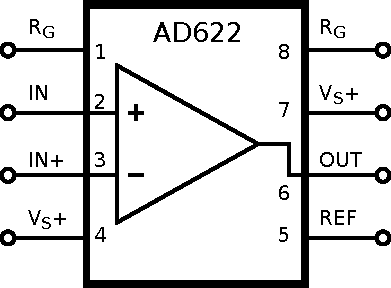
\includegraphics[width=0.260\textwidth]{../E05/latex/AD622.pdf}
  \end{center}
  \caption{Piedinatura dell'integrato AD622.}
  \label{cir5:ad622_piedinatura}
\end{wrapfigure}

In realtà, nell'esperienza abbiamo utilizzato un circuito integrato (più precisamente l'AD622, la cui piedinatura è esposta in Figura \ref{cir5:ad622_piedinatura}) che ha come qualità il fatto di avere un'alta precisione sul valore delle resistenze (abbiamo visto nel precedente circuito che uno squilibrio anche minimo fra i valori di resistenze che dovrebbero essere uguali può portare ad un guadagno diverso da quello teorico). Il suo guadagno è dato dall'equazione, fornita dal costruttore
$$G=1+\frac{50.5 \si{\kilo\ohm}}{R_g}$$

Una possibile applicazione di questo integrato è di utilizzarlo per individuare variazioni di tensione all'interno di un ponte di resistenze. Allo scopo, utilizziamo il circuito in Figura \ref{cir5:ad622_ponte}, con l'accortezza di portare una resistenza del ponte lontana dalle altre, così da poter modificarne la temperatura senza influenzare anche le altre.

Infatti, sappiamo che le resistenze hanno una dipendenza dalla temperatura data dal coefficiente di temperatura, che è di circa $200$ ppm/\si{\celsius}. Nel nostro caso, utilizzando come resistenza lontana dalle una da $100$ \si{\ohm}, la sua variazione per grado di temperatura sarà di $\Delta R / \Delta T= 100 \si{\ohm} (-200 \times 10^{-6}) = -20$ \si{\milli\ohm/\celsius}. Inoltre, per il ponte vale che non vi è differenza di tensione fra gli ingressi dell'integrato se il prodotto delle resistenze $R_1 R_4=R_2 R_3$: dunque, variando la resistenza $R_3$ inizieremo a registrare una tensione di uscita.

Sperimentalmente, si osserva però che una differenza di potenziale è già presente a temperatura ambiente (cioè senza variare la temperatura della resistenza $R_3$): questo fatto è imputabile al mancato bilanciamento del ponte. Infatti, è impossibile trovare due resistenze che abbiano un valore esattamente identico: dunque vi è un errore sistematico di cui dobbiamo tenere conto prima di effettuare le misure, fissando un valore zero di tensione, che si osserva essere $0.54$\si{\volt}.

Inoltre, la relazione che lega la variazione di tensione alla resistenza può essere calcolata considerando il ponte come l'insieme di due partitori (non scorre alcuna corrente verso l'amplificatore), cioè vale che
$$\Delta V = V^+ - V^- = V_d \left(\frac{R_4}{R_2+R_4}-\frac{R_2}{R_1+R_3}\right)$$

\begin{wrapfigure}[16]{r}{0.5\textwidth}
  \begin{center}
    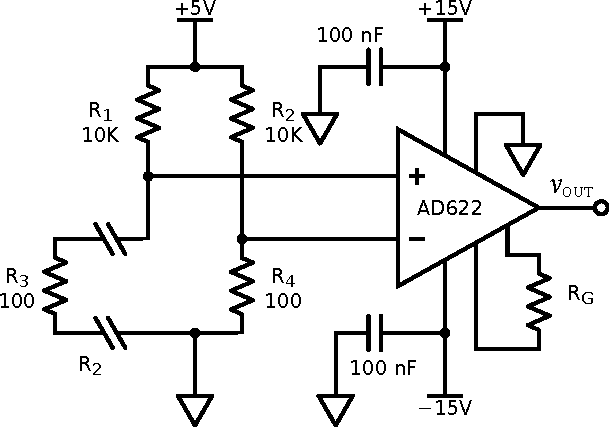
\includegraphics[width=0.40\textwidth]{../E05/latex/c_func_INA.pdf}
  \end{center}
  \caption{Circuito del ponte con l'amplificatore per strumentazione AD622. Le capacità sono state poste fra l'alimentazione e terra come per il $\mu$741.}
  \label{cir5:ad622_ponte}
\end{wrapfigure}

Considerando che l'uscita è amplificata dall'AD622 di un fattore di guadagno $A \approx 1000$ e $R_4/R_1<<1$, svolgendo i calcoli per $R_3=R_4+\Delta R$, otteniamo la seguente equazione
\begin{equation}
\Delta V_{out} = - A \frac{\Delta R}{R_1+R_4} V_{b}
\label{eq5:delta_R}
\end{equation}
dove $V_{b}$ è la tensione di alimentazione del ponte (come in Figura \ref{cir5:ad622_ponte}). Tenendo conto della relazione fra $\Delta R$ e la variazione di temperatura $\Delta T$, abbiamo che
\begin{equation}
\Delta T = \frac{\Delta R}{- 20 \si{\milli\ohm/\celsius}} = \frac{1}{20 \si{\milli\ohm/\celsius}} \frac{R_1+R_4}{V_b A} \Delta V
\label{eq5:delta_T}
\end{equation}

Presentiamo ora la tabella dei valori sperimentali con la modalità di variazione della temperatura. I valori di $\Delta V$ sono osservati, $\Delta R$ e $\Delta T$ sono calcolati rispettivamente con (\ref{eq5:delta_R}) e (\ref{eq5:delta_T}).

{\renewcommand{\arraystretch}{1.2}%
	\begin{tabular}{c|c|c|c}
    %\hline
	Modalità & $\Delta V$ [\si{\volt}] & $\Delta R$ [\si{\ohm}] & $\Delta T$ [\si{\celsius}]\\
    \hline
	Soffio & $0.08\pm0.01 $ & $0.16\pm0.03$ & $8.1 \pm 0.2$\\
    \hline
	Refrigerante & $-0.44\pm0.01 $ & $-0.88\pm0.06$ & $-44 \pm 3$\\
    %\hline
	\end{tabular}
}
\subsection{Misure di temperatura}

Nell'ultima parte dell'esperienza abbiamo eseguito misure di temperatura utilizzando una termoresistenza al platino PT100.
Essa non è altro che una resistenza di cui sono noti con sufficiente precisione alcuni parametri: il valore ad una data temperatura e il coefficiente di temperatura $\alpha$.
Sapendo che il valore di resistenza è dipendente dalla resistività elettrica del materiale $\rho$ che a sua volta dipende dalla temperatura (nel caso di metalli), secondo le seguenti relazioni:
	$$	R = \frac{\rho L}{S}
			\qquad \qquad
		\rho = \rho_0 \left[ 1 + \alpha \left( T - T_0 \right) \right]$$
dove L è la lunghezza del materiale e S la sezione, mentre $\rho$ dipende dalla resistività $\rho_0$ alla temperatura di riferimento $T_0$ e dal coefficiente di temperatura $\alpha$.
Combinando le due equazioni precedenti si ottiene la dipendenza del valore di resistenza dalla temperatura:
\begin{equation}
R = R_0 \left[ 1 + \alpha \left( T - T_0 \right) \right]
\end{equation}
Invertendo la formula si ottiene:
\begin{equation}
T = T_0 + \frac{1}{\alpha}\left( \frac{R}{R_0}-1 \right)
\end{equation}
\begin{wrapfigure}[15]{r}{0.45\textwidth}
\centering
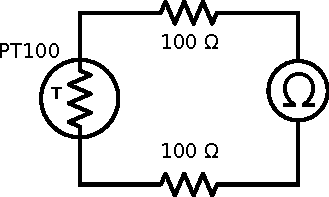
\includegraphics[width=.25\textwidth]{../E05/latex/c_PT100_2wire.pdf}
\caption{Circuito di controllo della temperatura a distanza: PT100 è il termoresistore al platino, l'ohmetro misura la resistenza in funzione della temperatura e le due resistenze da \SI{10}{\ohm} simulano i cavi lunghi.}
\label{cir5:2wire}
\end{wrapfigure}
Nel nostro caso il costruttore ci ha fornito i dati relativi alla temperatura di riferimento $T_0 =$ \SI{0}{\degreeCelsius}:
$$R_0 = \SI{100}{\ohm} \quad \quad \alpha = \SI[per-mode=symbol]{0.3850}{\ohm\per\degreeCelsius}$$

Conoscendo il comportamento della termoresistenza abbiamo simulato il caso in cui si volesse controllare la temperatura di un laboratorio a distanza.
I circuito che simulava questa situazione è riportato in Figura \ref{cir5:2wire}

Abbiamo notato subito che le misure ricavate con questo circuito soffrivano dell'errore sistematico dato dalle resistenze in serie da \SI{10}{\ohm}.
Infatti il valore di temperatura ricavato* era di XAKSJDKASJD \si{\degreeCelsius}, evidentemente errato.\\

Per evitare questo tipo di problemi abbiamo effettuato una misura a quattro fili.
In questa modalità il multimetro funzionava come generatore di corrente costante tramite due boccole e da voltmetro con le altre due boccole utilizzate.
Lo schema riportato in Figura \ref{cir5:4wire} mostra come la misura questa volta sia effettuata acquisendo la tensione ai capi della termoresistenza data dalla corrente del generatore.
In questa configurazione non vi è l'errore sistematico della misura a due fili, in quanto grazie all'alta impedenza del voltmetro, nella maglia interna non scorre corrente e pertanto ai capi delle resistenze su tale maglia non vi è alcuna caduta di potenziale.

\begin{wrapfigure}[15]{r}{0.45\textwidth}
\centering
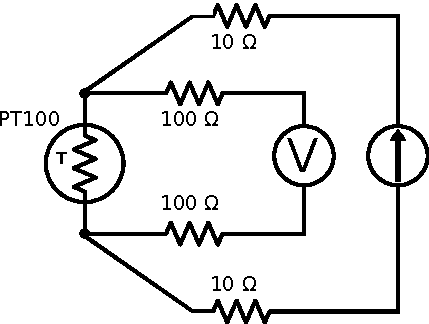
\includegraphics[width=.3\textwidth]{../E05/latex/c_PT100_4wire.pdf}
\caption{Configurazione di misura a quattro fili: nella maglia esterna scorre la corrente data dal generatore mentre nella maglia interna non scorre corrente. Il voltmetro ha un'impedenza idealmente infinita.}
\label{cir5:4wire}
\end{wrapfigure}

\subsection*{Conclusioni}
In questa esperienza abbiamo studiato alcuni circuiti utili a trasformare un segnale senza modificare l'informazione in esso contenuta: in particolare abbiamo esaminato circuiti raddrizzatori che non diminuiscono l'ampiezza del segnale come accade con i circuiti passivi quali i semplici diodi o il ponte raddrizzatore (ponte di Graetz).

Successivamente abbiamo studiato il cosiddetto amplificatore da strumentazione, in un circuito didattico costruito con un $\mu$A741 le cui limitazioni sono date dal guadagno fisso e dalla bassa impedenza in entrata e integrato in un dual inline package (AD622).
Ne abbiamo testato il funzionamento misurando lo sbilanciamento di un ponte di Wheatstone.

Infine abbiamo studiato una problematica di una misura a distanza data dalla lunghezza dei cavi.
Abbiamo risolto il problema con una misura a quattro fili.


\newpage

\setcounter{footnote}{0}

\section{22.10.2014 - Termostatazione}

In questa esperienza costruiremo un termometro elettronico utilizzando una Pt100. Realizzeremo poi un sistema di controllo proporzionale di temperatura utilizzando il termometro da noi costruito. 

\subsection*{Strumenti e materiali}

\begin{itemize} [noitemsep]
\item Oscilloscopio Agilent DSO-X 2002A (bandwidth \SI{70}{\mega\hertz}, sample rate \num{2} GSa/s);
\item Generatore di tensione continua Agilent E3631A (max $\pm \, \SI{25}{\volt}$ o $\pm \, \SI{6}{\volt}$);
\item Generatore di forme d'onta Agilent 33120A con range di frequenza da \SI{100}{\micro\hertz} a \SI{15}{\mega\hertz};
\item Multimetro Agilent 34410A a sei cifre e mezza;
\item Un amplificatore operazionale OP07;
\item Un integrato AD622;
\item Un integrato REF02;
\item Una termoresistenza PT100;
\item Transistor di potenza NPN 2N2222;
\item Resistenze e capacità di vari valori;
\item Trimmer multigiro da \SI{10}{\kilo\ohm} e \SI{1}{\kilo\ohm};
\item Breadboard e cablaggi vari.
\end{itemize}

\subsection{Termometro elettronico}

\subsection{Sistema di controllo proporzionale}

Aggiungiamo ora al circuito proposto nel paragrafo precedente un sistema di controllo proporzionale, la cui funzione sarà quella di riscaldare una resistenza fino a raggiungere una data temperatura di soglia.

Per comprenderne meglio l'implementazione, generalizziamo prima il concetto di controllo proporzionale. Osserviamo lo schema in Figura \ref : dati due segnali in ingresso X e R , il sistema deve rispondere con Y  se viene rispettata una condizione controllata dal nodo di confronto. Quest'ultimo avrà dunque il compito di confrontare X ed R e verificare che la condizione, in generale funzione dei due segnali, sia rispettata. L'aggiornamento di tale condizione è invece affidato al blocco di retroazione, che varia R.

Nel nostro caso, X è la tensione relativa alla temperatura di soglia (dunque dovremmo rispettare l'output del circuito precedente per impostarla, cioè $100$\si{\milli\volt\per\celsius}) e R la tensione relativa alla temperatura misurata dalla termoresistenza. La nostra Y sarà una data potenza dissipata su una resistenza di potenza che, se posta vicino alla PT100, varierà R, cioè la temperatura letta. Dobbiamo ora identificare i blocchi relativi al sistema di controllo proporzionale e progettare quelli mancanti nel circuito attuale.

Affidiamo il compito di blocco di retroazione al circuito finora costruito: questo restituisce un valore di tensione proporzionale alla temperatura letta dalla termoresistenza, che dovrà essere confrontato con la soglia. Successivamente, il blocco di controllo deve fare la differenza fra questi due valori e, una volta raggiungo un valore impostabile, diminuire il valore della corrente fornita alla resistenza di potenza in maniera proporzionale ad E. Definiamo dunque E=X-R, e per effettuare tale operazione utilizziamo un amplificatore differenziale . Infine, per fornire la corrente necessaria alla resistenza, utilizzeremo un transistor.

\subsubsection{Blocco di retroazione}
\subsection{...}

\subsection{...}

\subsection*{Conclusioni}

In questa esperienza abbiamo affrontato diverse problematiche, tra cui quella di progettare e costruire un circuiro composto di molte componenti.
Per fare ciò è stato necessario testare il funzionamento di singole parti dello schema complessivo per rendere più facile l'individuazione di eventuali problemi.

Nella prima parte dell'esperienza abbiamo assemblato un termometro elettronico utilizzando come sensore una termoresistenza PT100 e l'abbiamo tarato in modo tale che restituisse un valore di \SI{0}{\V} a \SI{0}{\celsius} e che scalasse di \SI{100}{\mV} ogni \SI{1}{\celsius}.

Nella seconda parte dell'esperienza invece abbiamo costruito un circuito di controllo proporzionale della temperatura.
Servendoci del primo circuito come fonte di informazione, abbiamo aggiunto due blocchi circuitali che facevano scorrere della corrente in una resistenza di potenza con il fine di riscaldare la resistenza PT100.
Inoltre questi nuovi blocchi regolavano o spegnevano l'alimentazione di tale resistenza di potenza una volta raggiunta una soglia di temperatura, decisa a priori.
In questo modo abbiamo creato un sistema termostatato ad una temperatura T da noi scelta.

In Figura \ref{gr6:grafico} è rappresentato l'andamento temporale della temperatura misurata dalla termoresistenza (in nero) e della temperatura di riferimento (in verde).
Come si può notare il tempo necessario alla resistenza di potenza per aumentare la temperatura da \SI{25}{\celsius} a \SI{32.5}{\celsius} dissipando energia per effeto Joule è di circa un minuto.
Una volta raggiunta la temperatura (in realtà come abbiamo visto l'alimentazione viene prima diminuita e poi tolta completamente) il circuito esclude l'alimentazione della resistenza di potenza, ma la temperatura registrata dalla PT100 continua a salire per inerzia termica dei componenti.
Dopo poco la temperatura registrata comincia a discendere verso la temperatura ambiente, ma, una volta scesa sotto la soglia, l'alimentazione della resistenza viene riattivata alzando nuovamente la temperatura della termoresistenza.
Questi passaggi vengono ripetuti e la temperatura oscilla asintoticamente vicino alla temperatura di soglia.

Si può osservare inoltre che la temperatura di riferimento ha una certa variabilità data dall'instabilità della tensione all'ingresso non invertente dell'opamp. Tale imperferzione è probabilmente generata da rumori ambientali.


\newpage

\setcounter{footnote}{0}

\section{28.10.2014 - Circuito per elettrocardiogramma (ECG)}

In questa esperienza costruiremo un circuito per effettuare un elettrocardiogramma (ECG).

\subsection*{Strumenti e materiali}

\begin{itemize} [noitemsep]
	\item Oscilloscopio Agilent DSO-X 2002A (bandwidth \SI{70}{\mega\hertz}, sample rate \num{2} GSa/s);
		\item Generatore di tensione continua Agilent E3631A (max $\pm \, \SI{25}{\volt}$ o $\pm \, \SI{6}{\volt}$);
		\item Multimetro Agilent 34410A a sei cifre e mezza;
		\item Due pile da \SI{9}{\volt};
		\item Due elettrodi;
		\item Amplificatori operazionali OP07;
		\item Un integrato AD622 e un ISO124;
		\item Resistenze e capacità di vari valori;
		\item Breadboard e cablaggi vari;
		\item Paziente (umano).
\end{itemize}

%\begin{wrapfigure}[20]{r}{0.24\textwidth}
%\centering
%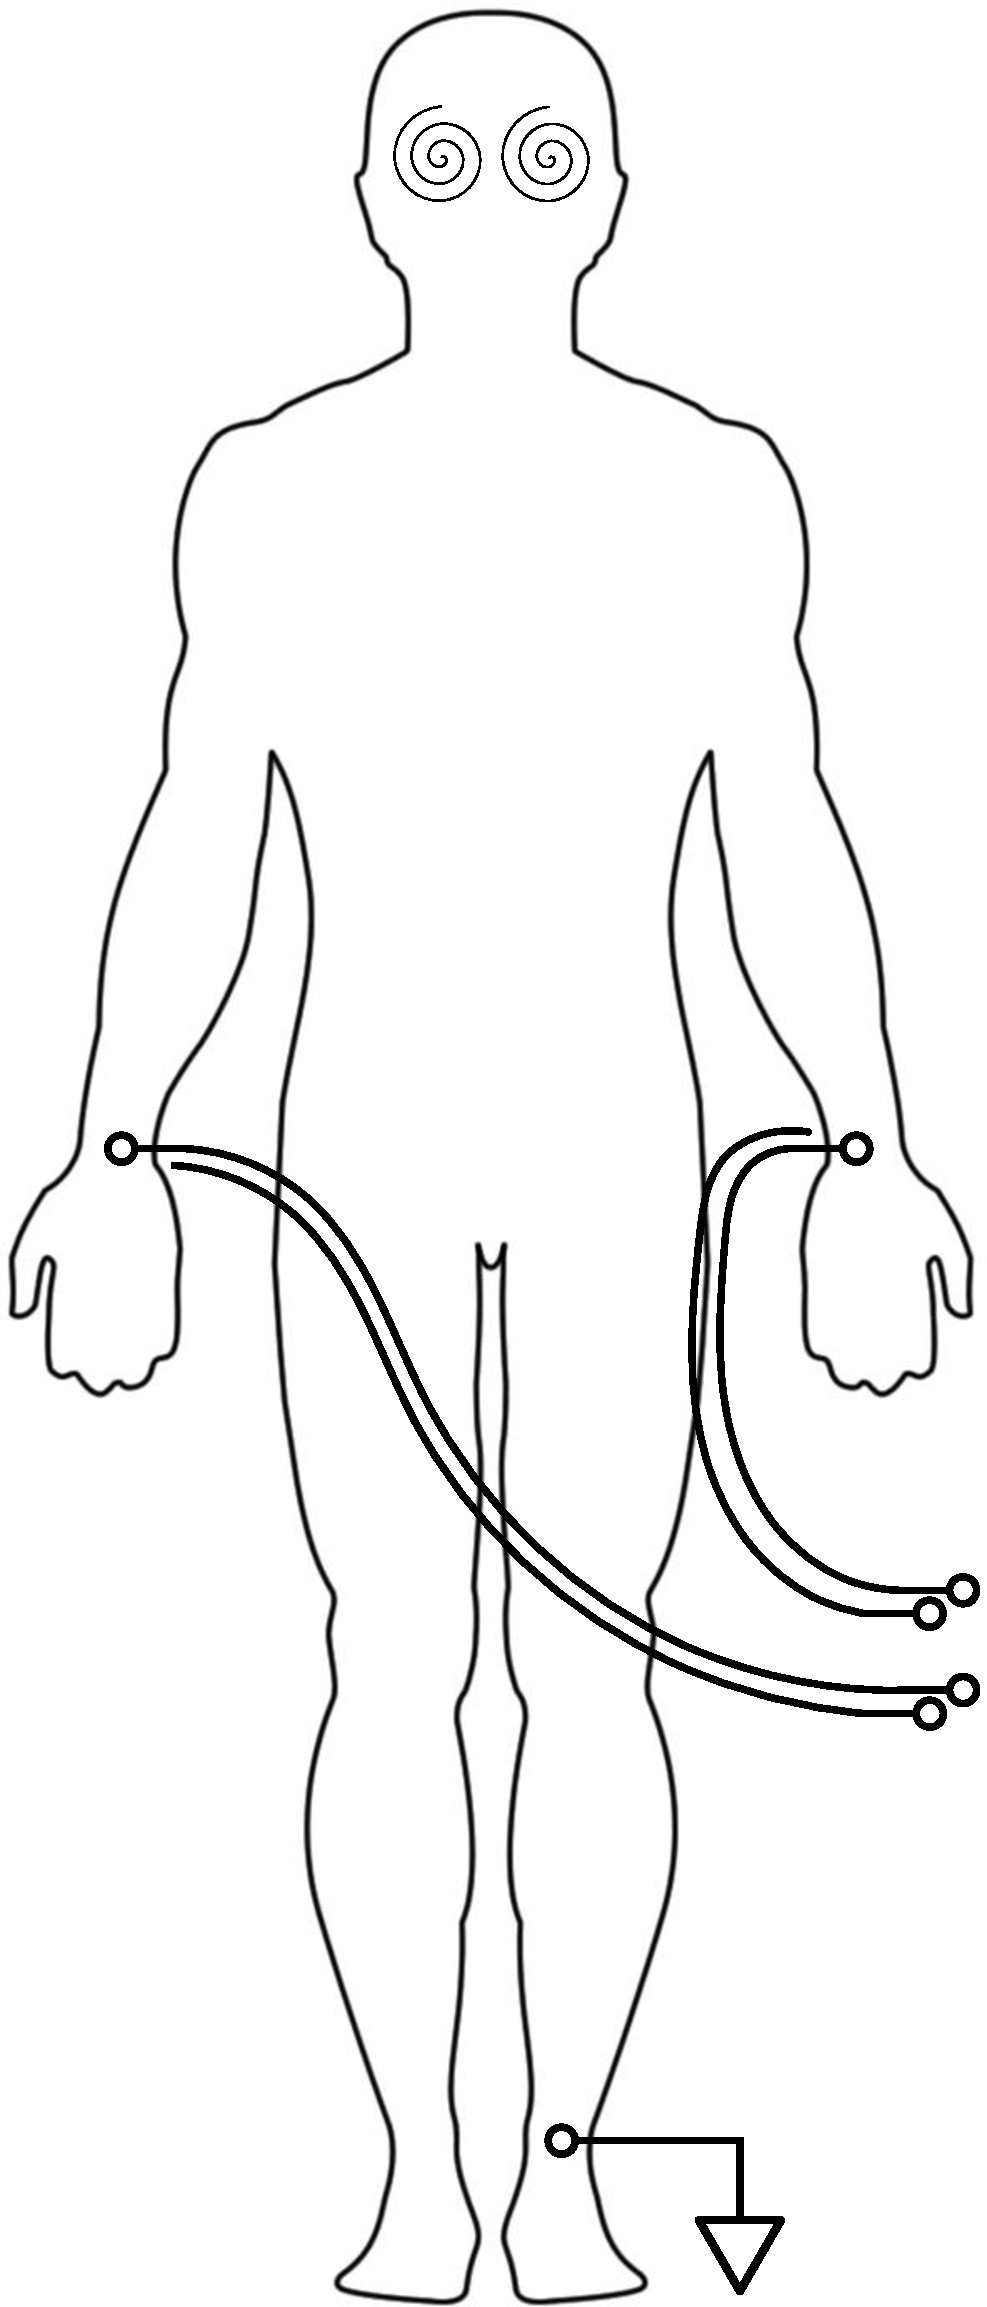
\includegraphics[width=.18\textwidth]{../E07/latex/human.pdf}%human.pdf}%doge.pdf}
%\caption{Connessioni al corpo poco umano di uno degli sperimentatori.}
%\label{fig7:human}
%\end{wrapfigure}

\subsection{Premesse}

Per progettare un circuito che legga il segnale elettrico del nostro battito cardiaco a livello della cute, dobbiamo considerare che:
\begin{itemize} [noitemsep]
	\item Sulla superficie del corpo il segnale ECG è normalmente di circa \SI{1}{mV} (al massimo raggiunge i \SI{4}{mV}) ed ha una frequenza di circa \SI{1.25}{\Hz}.
	\item Gli elettrodi a nostra disposizione, che realizzano il collegamento tra la strumentazione e il corpo, creano un potenziale di circa \SI{700}{\mV}, quindi circa \num{200} volte maggiore del segnale cardiaco.
	\item Il segnale da misurare è piccolo, quindi dobbiamo porre particolare attenzione alle fonti di rumore elettromagnetico dati da effetti capacitivi e/o induttivi. Inoltre dobbiamo evitare che i cavi e il paziente si muovano durante la misurazione.
	\item È necessario che il paziente sia isolato dal lato di elaborazione del segnale, alimentato dall'alimentatore da banco, per evitare problemi di giri di massa e pericoli per il paziente stesso dovuti a guasti degli apparecchi elettrici.
\end{itemize}

Tenendo conto di ciò, nei paragrafi successivi analizzeremo gli aspetti legati all'abbattimento dei rumori e all'amplificazione del segnale in ingresso.

\subsection{Abbattimento dei rumori}

\subsubsection*{Operazionale U1}

Con il primo stadio in entrata (operazionale U1 in Figura \ref{cir7:elettro-cardiogramma}) eliminiamo i segnali di modo comune generati dagli elettrodi (oltre ad avere un'alta impedenza in ingresso e quindi un valore in entrata ad U1 più fedele alla reale ddp generata dal corpo). In testa ed in coda a questo stadio sono anche presenti delle capacità che creano due filtri: rispettivamente un passa basso ed un passa alto.

\paragraph*{Passa Basso}
Posto in testa ad U1, e composto dalle capacità $C_c$ e $C_d$, è necessario per abbattere eventuali rumori ambientali. Inserendo le capacito nel circuito come in Figura \ref{cir7:elettro-cardiogramma}, il datasheet dell'operazionale ci fornisce direttamente le frequenze di taglio di modo differenziale
\begin{equation*}
	\frac{1}{2 \pi R ( C_d + C_c ) } = \SI{194}{\Hz}
\end{equation*}
e di modo comune
\begin{equation*}
	\frac{1}{2 \pi R C_c} = \SI{4}{\kHz}
\end{equation*}

Con queste capacità riusciamo dunque ad eliminare i segnali di modo comune ad alte frequenze, ma soprattutto tagliamo ogni frequenza superiore ai \SI{200}{\Hz} in modo differenziale (il nostro segnale è infatti sui \SI{1.25}{\Hz} come da premesse), e dunque restringiamo drasticamente le frequenze ammesse ad essere amplificate dal nostro circuito.

\paragraph*{Passa Alto}
Essendo posto all'uscita dell'operazionale (capacità $C_1$ in Figura \ref{cir7:elettro-cardiogramma}), elimina eventuali segnali continui in output. La sua frequenza di taglio è di circa \SI{3}{\Hz}. Inoltre, è necessario che l'impedenza siano adattate, ovvero dovrà essere vista come infinita in entrata al prossimo blocco: per far ciò poniamo un ulteriore operazionale (un OP07, U2 in Figura \ref{cir7:elettro-cardiogramma}).

\subsubsection*{Operazionale U3 ed active gards}

Per diminuire l'effetto dei segnali di modo comune (dovuto agli elettrodi), è conveniente polarizzare in maniera uguale entrambe le calze dei cavi coassiali utilizzati per la connessione elettrodo-amplificatore. Così facendo il potenziale delle calze rimarrà uguale indipendentemente da eventuali movimenti dei cavi. Inoltre la differenza di potenziale fra la calza e il cavo che trasporta il segnale sarà minimizzata al fine di limitare le perdite sull'isolante.

Per effettuare la polarizzazione dobbiamo dunque attingere ad una tensione di $\approx \SI{700}{\milli\volt}$. Quindi abbiamo scelto di utilizzare la media fra i segnali entranti che, dato l'alto valore del segnale in modo comune, sarà la tensione desiderata. Infatti, se ricordiamo la struttura interna dell'amplificatore per strumentazione (Figura \ref{cir5:instr_amplif}), notiamo che, passando la stessa corrente sulle resistenze $R_1$ e su $R_G$, il punto ad $1/2 R_G$ è proprio a metà fra la due tensioni in ingresso.

\subsubsection*{Pile e amplificatore di isolamento}

Per alimentare il circuito abbiamo optato per utilizzare due pile da \SI{9}{\volt}, e come comune il polo positivo di una collegato al polo negativo dell'altra. Questo ha permesso di abbattere tutti i rumori relativi all'alimentazione dell'edificio e di avere una comune flottante rispetto a quella dell'oscilloscopio (in nero nella Figura \ref{cir7:elettro-cardiogramma}).

Per isolare ulteriormente il circuito ed evitare giri di massa abbiamo anche utilizzato un ISO124. Questo operazionale ha le seguenti caratteristiche
\begin{itemize}[noitemsep]
	\item Isola fino a \SI{1500}{\volt} e ammette una alimentazione da $\pm$ 4,5V a $\pm$ 18V;
	\item Possiede due alimentazioni separate e quindi anche due riferimenti di massa indipendenti l'uno dall'altro.
\end{itemize}

\begin{figure}[tpc]
\centering
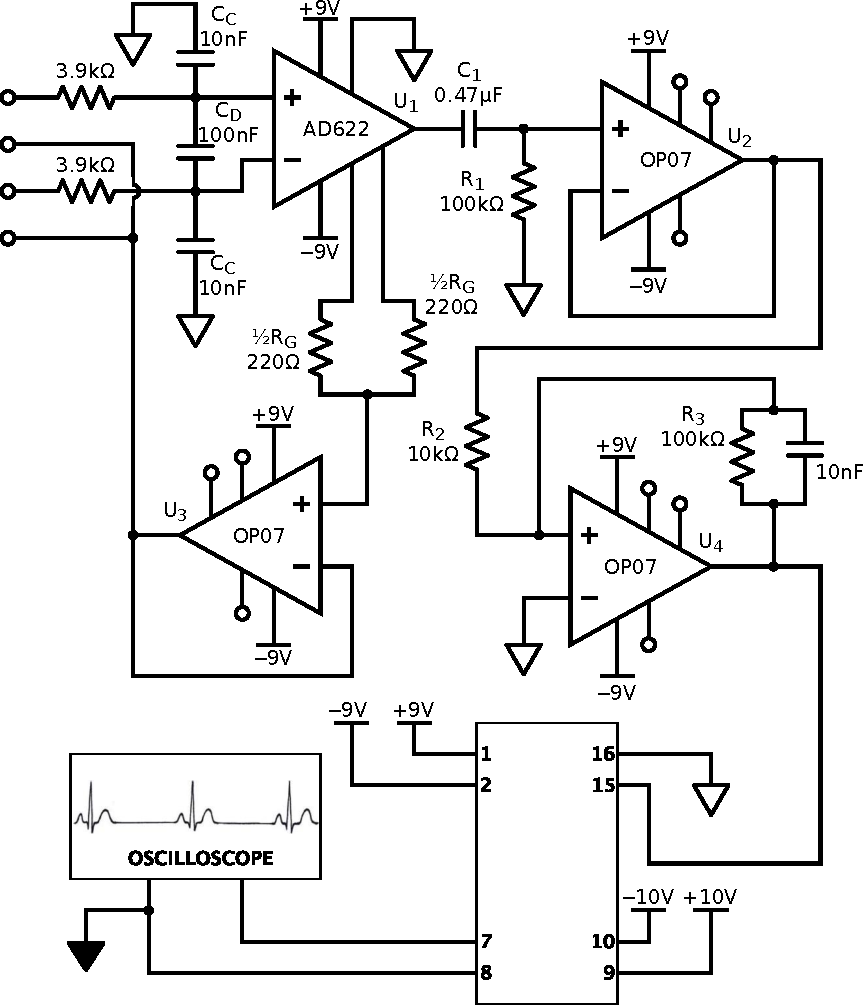
\includegraphics[width=.6\textwidth]{../E07/latex/circuito.pdf}
\caption{Schema del circuito da noi utilizzato per l'elettrocardiogramma.}
\label{cir7:elettro-cardiogramma}
\end{figure}

\subsection{Amplificazione}

Dato il basso valore di tensione del segnale in entrata, abbiamo anche la necessità di amplificarlo per permettere alla strumentazione di leggerlo. Nel circuito ci sono tre stadi di amplificazione che amplficano il segnale di circa 800 volte.

\subsubsection*{Operazionale U1}
L'AD622, come visto nell'Esperienza 5, controlla l'amplificazione tramite la presenza di una resistenza posta nei punti dedicati della piedinatura (si faccia riferimento alla Figura \ref{cir5:ad622_ponte}). Con le resistenze utilizzate, l'amplificazione è data dalla legge  fornitaci dal costruttore
$$G_1=1+\frac{50.5 \si{\kilo\ohm}}{R_g} \approx 116$$

\subsubsection*{Filtro passa alto}
Con la sua frequenza di taglio di circa \SI{3}{\Hz}, il filtro passa alto in coda ad U1 riduce il nostro segnale (in uscita dal primo stadio di amplificazione dato da U1). Possiamo stimare di quanto viene ridotto considerando la funzione di partizione di un passa alto e facendone il modulo, ottenendo il guadagno. Vale dunque che
$$G_2=\frac{2 \pi R_1 C_1 \times \SI{1.25}{\Hz}}{\sqrt{1+(2 \pi R_1 C_1 \times \SI{1.25}{\Hz})^2}}\approx 0.35$$

\subsubsection*{Operazionale U4}
Questo operazionale è posto in un blocco con retroazione negativa non invertente. Dunque il suo guadagno è dato da
$$G_3=1+\frac{R_2}{R_3} \approx 11$$

L'amplificazione totale è dunque
$$G = G_1 \times G_2 \times G_3 \approx 450$$

La capacità di \SI{10}{\nano\farad} inserita è un ulteriore stadio di abbattimento dei rumori ad alte frequenze.


\begin{figure}[htpc]
\centering
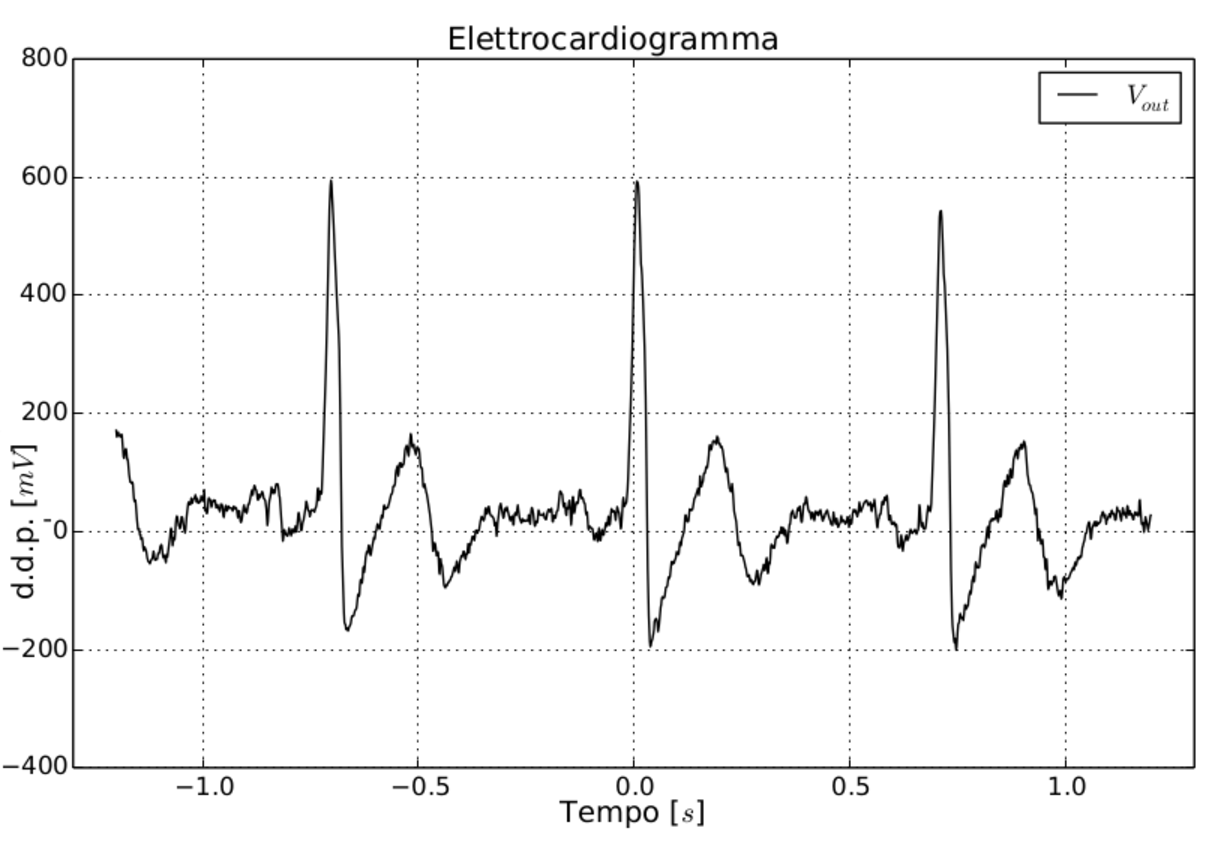
\includegraphics[width=.7\textwidth]{../E07/latex/g4.pdf}
\caption{Grafico della tensione registrata dall'oscilloscopio in funzione del tempo (ECG).}
\label{fig7:ecg_output}
\end{figure}

\subsection*{Conclusioni}
In questa esperienza siamo riusciti ad ottenere un elettrocardiogramma affetto da poco rumore, grazie agli stadi di abbattimento inseriti, e amplificato in maniera tale da poter essere osservato sull'oscilloscopio.


\newpage

\setcounter{footnote}{0}

\section{05.11.2014 - Oscillatore a ponte di Wien}

In questa esperienza construiremo un circuito oscillante detto \textit{oscillatore a ponte di Wien} ed effettueremo una pole-zero compensation di una sonda per oscilloscopio.

\subsection*{Strumenti e materiali}

%\begin{figure}[htc]
\begin{itemize} [noitemsep]
	%\item Generatore di forme d'onta Agilent 33120A con range di frequenza da \SI{100}{\micro\hertz} a \SI{15}{\mega\hertz};
	\item Oscilloscopio Agilent DSO-X 2002A (bandwidth \SI{70}{\mega\hertz}, sample rate \num{2} GSa/s);%\newline
%	\begin{minipage}{0.65\textwidth}
%		\vspace{0.4mm}
%%		\begin{itemize} [noitemsep]
%%		\item Oscilloscopio Agilent DSO-X 2002A (bandwidth \SI{70}{\mega\hertz}, sample rate \num{2} GSa/s);
		\item Generatore di tensione continua Agilent E3631A (max $\pm \, \SI{25}{\volt}$ o $\pm \, \SI{6}{\volt}$);
%%		\item Generatore di forme d'onta Agilent 33120A con range di frequenza da \SI{100}{\micro\hertz} a \SI{15}{\mega\hertz};
		\item Multimetro Agilent 34410A a sei cifre e mezza;
		\item Amplificatore operazionale $\mu$A741;
		\item Una lampadina a filamento;
		\item Resistenze e capacità di vari valori;
		%\item Trimmer multigiro da \SI{10}{\kilo\ohm} e \SI{1}{\kilo\ohm};
		\item Breadboard e cablaggi vari.
		\item Una sonda compensata
%%		\end{itemize}
%	\end{minipage}
%	\begin{minipage}{0.3\textwidth}
%			\centering
%			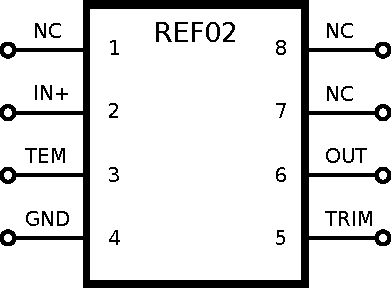
\includegraphics[width=3.5cm]{../E06/latex/REF02.pdf}
%			\caption{Piedinatura dell'integrato\newline REF02.}
%			\label{cir6:REF02}
%	\end{minipage}
\end{itemize}
%\end{figure}
%\vspace{-.8cm}

\begin{wrapfigure}[15]{r}{0.45\textwidth}
\centering
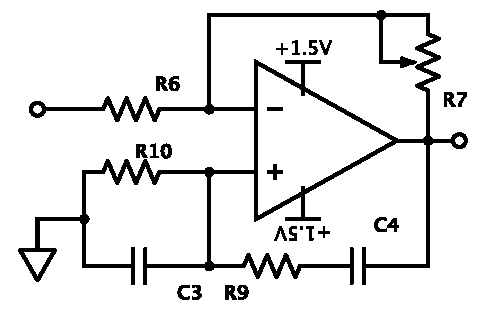
\includegraphics[width=.35\textwidth]{../E08/latex/osc.pdf}
\caption{Schema dell'oscillatore a ponte di Wien senza regolazione del guadagno.}
\label{cir8:without_lamp}
\end{wrapfigure}

\subsection{Oscillatore a ponte di Wien}

L'idea alla base dell'oscillatore a ponte di Wien è quella di sfruttare la selezione in frequenza di un filtro passa banda - il ponte di Wien - caratterizzato da avere il massimo guadagno per una determinata frequenza $f_0$.

All'accensione dell'alimentazione del circuito si crea una forma d'onda quadra che contiene tutte le frequenze e pertanto anche $f_0$ (un'onda quadra puù essere ottenuta tramite serie di Fourier).

Dunque, se riusciamo a stabilizzare il circuito, ovvero evitare che nel tempo o si smorzi o vada in saturazione, avremo una oscillazione alla frequenza $f_0$ e con ampiezza costante. Dovremo dunque imporre un guadagno complessivo unitario.


%Ciò significa che, imponendo unitario il guadagno massimo del circuito, si otterrà un circuito che oscilla con ampiezza costante a $f_0$, con l'ampiezza data dall'ampiezza iniziale.

Lo schema in Figura \ref{cir8:without_lamp} presenta il circuito con amplificazione massima unitaria.
Come si può vedere esso è composto da un opamp con due rami di retroazione negativa e positiva.
Il ramo di feedback positivo è dato dal ponte di Wien mentre quello negativo è composto da un partitore resistivo.

Analizzando il circuito per $\omega_0=2\pi f_0=\frac{1}{RC}$ ($s=\frac{j}{RC}$) otteniamo dai due partitori:

\begin{equation}
  \begin{array}{lr}
	V^+_{f_0} = \frac{Z_{//}}{Z_1 + Z_{//}}V_{out} = \frac{1}{3}V_{out}\\
	V^-_{f_0} = \frac{R_1}{R_1+R_2}V_{out}
  \end{array} \bigg\}
\quad dove \quad %\intertext{dove}
\Bigg\{
  \begin{array}{lr}
	Z_1 := \frac{sRC+1}{sC}\\
	Z_{//} := \frac{R}{1+sRC}\\
	s = s_0 = \frac{2\pi}{RC}
  \end{array}
\end{equation}

Inserendo $V^+$ e $V^-$ nell'espressione del guadagno di un opamp si ottiene
\vspace{-2mm}
\begin{equation}
	V_{out,f_0} = A_{ol}\left( V^+_{f_0} - V^-_{f_0} \right) = A_{ol}\left(\frac{R_1}{R_1+R_2} - 1/3\right)V_{out,f_0}
\end{equation}
\vspace{-4mm}
da cui, per $A_{ol} \rightarrow \infty$, semplificando $V_{out,f_0}$

\begin{equation}
	R_2 = 2 R_1
\end{equation}

Utilizzando questi componenti otteniamo pertanto un sistema che oscilla alla frequenza $f_0$.
La problematica di tale circuito è però che non abbiamo il controllo dell'ampiezza dell'oscillazione. Se idealmente infatti troviamo una $R_2 = 2 R_1$, allora avremo in uscita un segnale oscillante con frequenza $f_0$ ma con ampiezza dipendente dal segnale iniziale in ingresso. Ricordando che il segnale in ingresso è verosimilmente un onda quadra, l'ampiezza del segnale a frequenza $f_0$ sarà dato dal relativo coefficiente della serie di Fourier. Avremo dunque un segnale sicuramente piccolo (pochi \si{\milli\volt}). Se scegliamo un guadagno maggiore de 1, il nostro segnale verrà amplificato fino a quando l'intero sistema non va in saturazione. Dobbiamo dunque trovare un modo di regolare il guadagno in base all'ampiezza del segnale. Al contrario, se il guadagno è minore di 1, il nostro segnale si smorzerà con il passare del tempo. 

\subsubsection*{Controllo automatico del guadagno}

La configurazione precedente è detta autoinnescante, cioè basta alimentare l'opamp affinché il circuito inizi ad oscillare.
Per avere un innesco certo è però necessario che il guadagno totale del circuito sia \textit{inizialmente} maggiore di \num{1}. Così facendo, avremo un'amplificazione del piccolo segnale in ingresso.

Per fare ciò si sostituisce la resistenza $R_1$ con una lampadina a filamento (il nuovo circuito è proposto in Figura \ref{cir8:with_lamp}).
Essa infatti possiede una coefficiente di temperature postivo non lineare che ne aumenta la resistenza con l'aumento temperatura, generato per effetto joule dalla corrente.

\begin{wrapfigure}[10]{l}{0.45\textwidth}
\centering
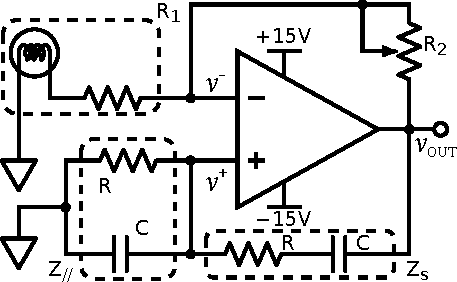
\includegraphics[width=.35\textwidth]{../E08/latex/osc_w_lamp.pdf}
\caption{Schema dell'oscillatore a ponte di Wien con regolazione del guadagno ottenuta mediante una lampadina a filamento.}
\label{cir8:with_lamp}
\end{wrapfigure}

Inizialmente la resistenza sarà più fredda e pertanto il guadagno del circuito sarà maggiore di \num{1}, innescando l'oscillazione.
Con il passaggio di corrente nella lampadina, essa si scalderà e aumenterà la propria resistenza, diminuendo il guadagno portandolo a valori inferiori di \num{1}.
Ciò porterà il circuito a stabilizzarsi con un guadagno unitario e pertanto a generare un'oscillazione di frequenza $f_0$ di ampiezza costante.

Utilizzando un trimmer è possibile aggiustare il valore della resistenza $R_2$ in modo che l'oscillazione autosostenuta del ponte di Wien abbia l'ampiezza desiderata.

$$$$
$$$$

\begin{figure}[htpc]
\centering
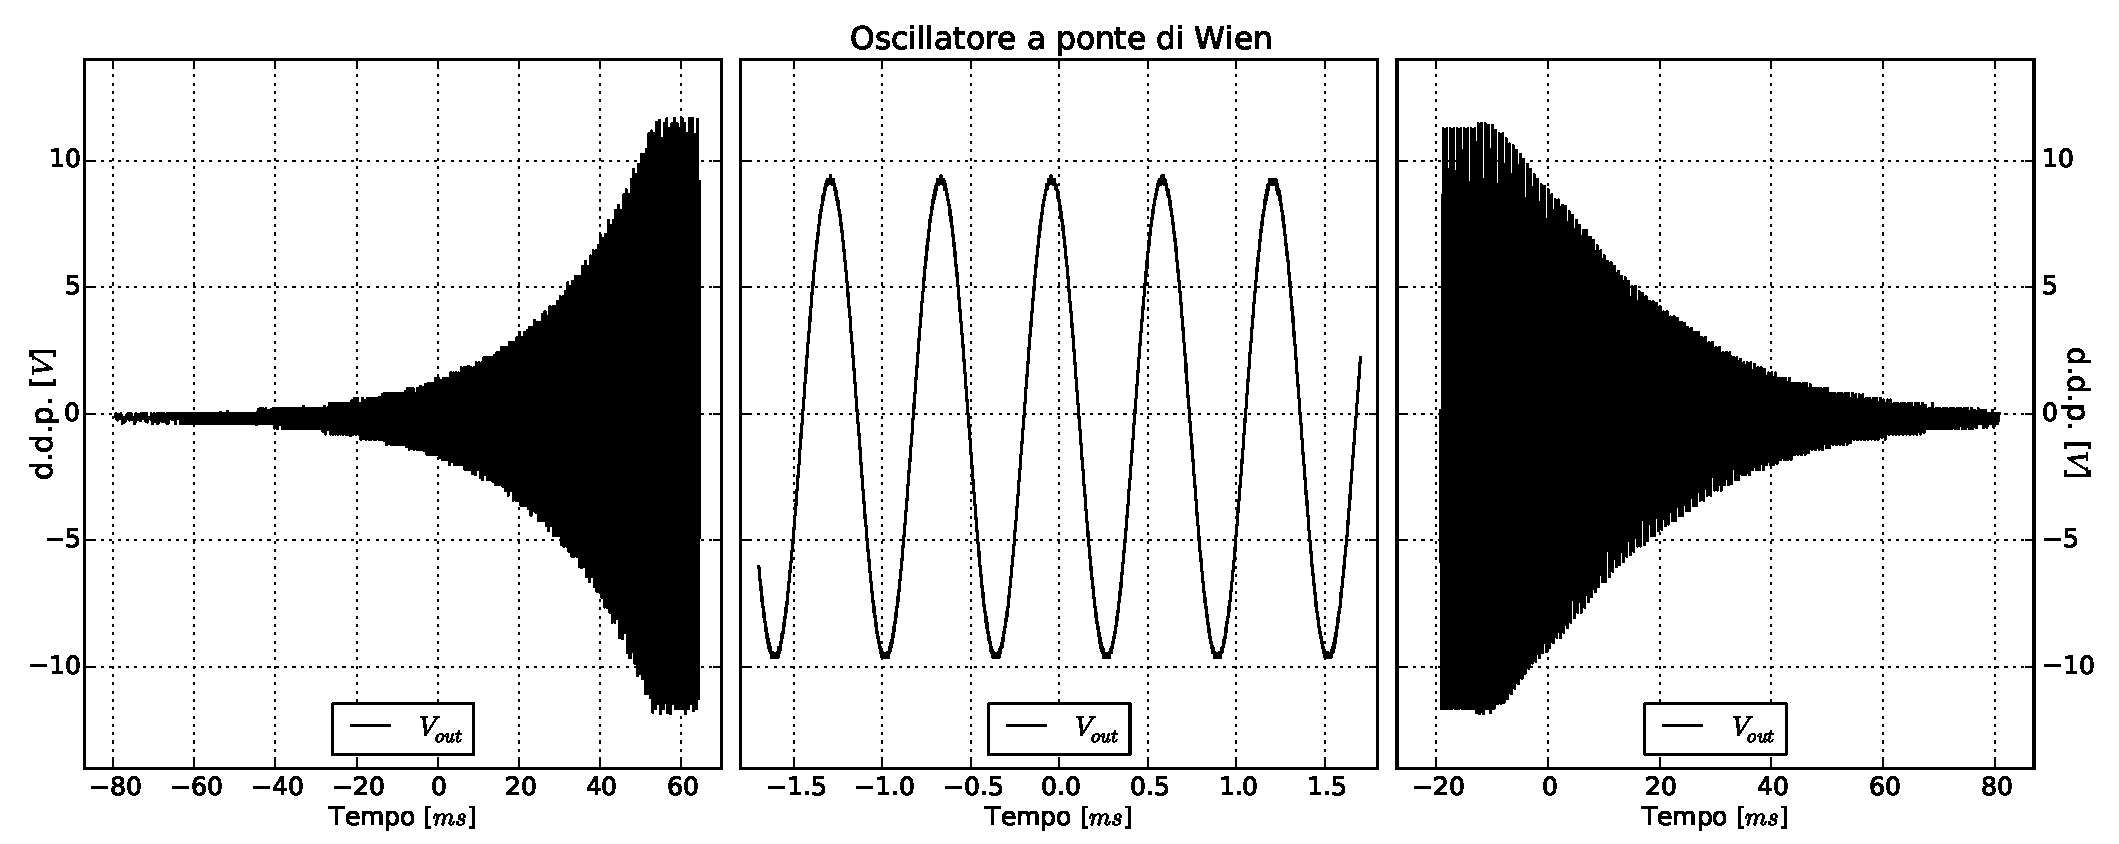
\includegraphics[width=.95\textwidth]{../E08/latex/wien.pdf}
\caption{Risposta del circuito oscillatore, nel grafico a sinistra in guadagno è maggiore di \num{1}, nel grafico centrale il guadagno è stabile, nel grafico a destra il guadagno è inferiore di \num{1}.}
\label{fig8:wien}
\end{figure}

\subsection{Pole-zero compensation di una sonda}

La \textit{pole-zero compensation} è una tecnica che permette di compensare dei poli del sistema. Tale procedimento ci permette di eliminare dipendenze dalla grequenza e di effettuare misure precise di circuiti senza interferenze da parte dell'apparato di misura.

Essa consiste nel posizionare, aggiungendo un'ulteriore parte circuitale, uno zero alla funzione di trasferimento esattamente nel punto in cui esiste un polo .
In equazioni si traduce con:

\[
  \begin{array}{lr}
H(s) = \frac{a(s)}{b(s)} \quad tc \quad b(s_0) = 0 \\
f(s) \quad tc \quad f(s_0) = 0
  \end{array}\left\}
\quad \longrightarrow \quad H'(s) = \frac{a(s)f(s)}{b(s)} \quad tc \quad H'(s_0) = 0
\right.
\]

Per ottenere questo risultato, si antepone all'oscilloscopio una sonda compensata il cui circuito schematizzato è proposto in Figura \ref{cir8:probe}.

\begin{wrapfigure}[13]{r}{0.45\textwidth}
\centering
\includegraphics[width=.35\textwidth]{../E08/latex/probe.pdf}
\caption{Schema del circuito di misura composto dall'oscilloscopio e dalla sonda.}
\label{cir8:probe}
\end{wrapfigure}
Come si può notare la sonda e l'oscilloscopio formano un partitore e pertanto la tensione misurata dallo strumento non sarà la stessa del circuito.
Sarà determinata dalla funzione di trasferimento:

\begin{equation}
H(s)=\frac{Z_{osc}}{Z_{probe}+Z_{osc}} = \frac{R_2}{R_1+R_2}\,\frac{1+R_1C_1s}{1+\frac{R_1R_2}{R_1+R_2}(C_1+C_2)s}
\end{equation}

Da questa formula è evidente che la compensazione del polo sia ha quando la seconda frazione è uguale ad \num{1} e quindi il partitore diventa completamente resistivo:
\begin{equation*}
1+R_1C_1s = 1+\frac{R_1R_2}{R_1+R_2}(C_1+C_2)s
\end{equation*}
da cui
\begin{equation}
R_1 = R_2 \frac{C_2}{C_1}
\end{equation}

Questa relazione permette di spostare lo zero della sonda proprio sul polo dell'oscilloscopio permettendone la compensazione.
Dal punto di vista pratico, rendiamo la sonda insensibile alla frequenza e, fissati i parametri $R_2$, $C_2$ e $C_1$, si varia $R_1$ finché l'oscilloscopio non misura la stessa tensione $V_{in}$ ridotta di un fattore $\frac{R_2}{R_1+R_2}$.

\begin{figure}[htpc]
\centering
\includegraphics[width=.65\textwidth]{../E08/latex/compensation.pdf}
\caption{Risposta del circuito composto dalla sonda e dall'oscilloscopio visto dall'oscilloscopio stesso. La sonda è stata eccitata con un'onda quadra tramite il generatore interno dell'oscilloscopio.}
\label{fig8:compensation}
\end{figure}

\subsection*{Conclusioni}
In questa esperienza abbiamo costruito un circuito che, come l'oscillatore a rilassamento, fornisce un'oscillazione autosostenuta. La cosa interessandte del ponte di Wien è che la forma d'onda in uscita è praticamente sinusoidale. Ciò può essere utile per applicazioni dove si necessità di una forma d'onda di tale tipo. Nella seconda parte dell'esperienza abbiamo compesato una sonda. Tali sonde sono molto utili per il fatto che sono insensibili alla frequenza del segnale. Se andiamo a rivedere l'Esperienza 3, nel grafico \ref{gr3:slew_rate} vediamo come l'onda quadra in ingresso non sia perfetta. Ciò è dovuto ad un effetto di sovracompensazione della sonda (in quel caso un semplice cavo). Dunque, per esperimenti che riguardano segnali ad alta frequenza o che contengono alte frequenze (onda quadra), è preferibile utilizzare sonde compensate.

\newpage

\setcounter{footnote}{0}

\section{11.11.2014 - Porte logiche - Prima Parte}

In questa esperienza verificheremo il funzionamento di alune porte logiche TTL e semplici circuiti costruiti con esse.

\subsection*{Strumenti e materiali}

\begin{itemize} [noitemsep]
	\item Oscilloscopio Agilent DSO-X 2002A (bandwidth \SI{70}{\mega\hertz}, sample rate \num{2} GSa/s);
	\item Generatore di tensione continua Agilent E3631A (max $\pm \, \SI{25}{\volt}$ o $\pm \, \SI{6}{\volt}$);
	\item Multimetro Agilent 34410A a sei cifre e mezza;
	\item Un integrato 7400, composto di quattro porte logiche TTL NAND; % '00;
	\item Basetta a LED;		
	\item Resistenze e capacità di vari valori;
	\item Breadboard e cablaggi vari.
\end{itemize}

\subsection{Logiche TTL e scheda di visualizzazione}

Le porte logiche a tecnologia TTL funzionano utilizzando come 1 logico il valore di tensione +\SI{5}{\volt} mentre come 0 logico \SI{0}{\volt}.
Pertanto l'alimentazione che porteremo alla breadboard non sarà più $\pm$\SI{15}{\V} e GND, ma solo $+$\SI{5}{\V} e GND.
Ricordiamo che l'alimentazione deve essere stabilizzata e disaccoppiata con i condensatori come nel caso analogico in quanto nei momenti di commutazione delle porte abbiamo grandi variazioni di tensione in piccoli tempi (idealmente la variazione da stato 1 a 0 è istantanea).
È dunque essenziale avere una riserva di cariche utilizzabili dal circuito nel momento in cui si hanno commutazioni.

Per controllare il funzionamento dei nostri circuiti utilizzeremo una schedina di visualizzazione a led fornitaci già assemblata.
Essa permette di visualizzare lo stato "alto" o "basso" delle linee da monitorare tramite 8 led (4 rossi e 4 verdi).
Tali schede contengono un integrato buffer 74LS244 nella logica TTL che fornisce in uscita una corrente di \SI{-15}{\milli\ampere} per il livello alto e di \SI{24}{\milli\ampere} per il livello basso.

\subsubsection{Porta NAND}

Abbiamo verificato il funzionamento di una porta NAND utilizzando, come già detto, una scheda di visualizzazione a LED.
È stata verificata la seguente tavola di verità.\\

\begin{figure}[htpc]
\centering
	\begin{subfigure}[hc]{.4\textwidth}
		\centering
		{\renewcommand{\arraystretch}{1.2}%
		\begin{tabular}{|c|c|c|}
		\hline
		A & B & $\overline{AB}$ \\
		\hline
		0 & 0 & 1\\
		\hline
		0 & 1 & 1\\
		\hline
		1 & 0 & 1\\
		\hline
		1 & 1 & 0\\
		\hline
		\end{tabular}}
		\label{tab9:NAND}
        \end{subfigure}
        \begin{subfigure}[hc]{.4\textwidth}
		\centering
		\includegraphics[width=.35\textwidth]{../E09/latex/NAND.pdf}
		\label{cir9:nand}
        \end{subfigure}
\caption{Tabella di verità e simbolo circuitale convenzionalmente utilizzato per porte NAND.}
\end{figure}

\subsubsection{Porta NOT}

\begin{wrapfigure}[10]{r}{0.4\textwidth}
\centering
\includegraphics[width=.16\textwidth]{../E09/latex/NOT.pdf}
\caption{Implementazione e simbolo circuitale per porte NOT.}
\label{cir9:not}
\end{wrapfigure}

Non avendo a disposizione una porta NOT, abbiamo utilizzato una porta NAND cortocircuitando i due ingressi tra loro.
Così facendo otteniamo un'implementazione di una porta NOT.

Ne abbiamo ininzialmente verificato il funzionamento collengandola alla scheda di visualizzazione led e fornendo un'onda quadra in ingresso ($V_{pp}=\SI{5}{\volt}$, $V_{off}=+\SI{2.5}{\volt}$, $\nu=\SI{2}{\hertz}$).
Una volta eseguito questo test preliminare, abbiamo collegato ingresso ed uscita all'oscilloscopio e ne abbiamo analizzato la risposta per diverse tensioni costanti in ingresso.
I dati ottenuti sono riportati in Tabella (\ref{tab9:risposta2}).
Come vediamo, tra \SI{1}{\volt} e \SI{1.5}{\volt} la tensione varia in modo molto rapido.

\vspace{2mm}
\begin{table}[htpc]
\centering
{\renewcommand{\arraystretch}{1.1}%
\begin{tabular}{|l|c|c|c|c|c|c|c|c|c|c|c|}
\hline
$V_{in}$ [\si{\volt}] & 0.0 & 0.5 & 1.0 & 1.5 & 2.0 & 2.5 & 3.0 & 3.5 & 4.0 & 4.5 & 5.0 \\
\hline
$V_{out}$ [\si{\volt}] & 4.30 & 4.05 & 3.01 & 0.10 & 0.10 & 0.10 & 0.10 & 0.10 & 0.10 & 0.10 & 0.10 \\
\hline
\end{tabular}}
\caption{I valori sono stati ricavati variando la tensione in entrata di \SI{.5}{\V}.}
\label{tab9:risposta2}
\end{table}

Siamo dunque interessati a capire meglio la risposta della porta in funzione della tensione in ingresso.
Per fare ciò utilizziamo la modalità XY dell'oscilloscopio.

Abbiamo dunque fornito un'onda sinusoidale all'ingresso di frequenza \SI{100}{\kilo\hertz}, $V_{pp}=\SI{5}{\volt}$ e $V_{off}=+\SI{2.5}{\volt}$.
Come vediamo dal grafico sotto riportato, sebbene stiamo lavorando con segnali digitali (1 o 0) le tensioni in gioco sono manifestamente analogiche.
Avremo dunque tutta la serie di problemi già affrontati nella parte analogica del corso.
Vediamo infatti che la tensione in uscita non è una funzione a gradino.
Inoltre, per evitare che rumori molesti disturbino il segnale in uscita, avremo bisogno di una sorta di isteresi.
Non esisterà dunque un valore ben definito di V alta e V bassa, ma delle bande di lavoro standard per la classe di circuiteria scelta (nel nostro caso TTL), riportate solitamente nel data-sheet.
Lo standard TTL è riportato in Figura \ref{fig9:TTL}

\begin{figure}[htpc]
\centering
	\begin{subfigure}[hc]{0.49\textwidth}
		\centering
		\includegraphics[width=.95\textwidth]{../E09/latex/XY.pdf}
                \caption{Risposta in uscita di una porta NAND con entrate cortocircuitate (= NOT) ad un'onda triangolare di frequenza \SI{100}{\kHz} in entrata.}
                \label{fig9:XY}
        \end{subfigure}%
	\quad
        \begin{subfigure}[hc]{0.49\textwidth}
		\centering
		\includegraphics[width=.95\textwidth]{../E09/latex/TTL.png}
                \caption{Livelli standard di input e output per la logica TTL.}
                \label{fig9:TTL}
        \end{subfigure}
\caption{}
\end{figure}
\vspace{-5mm}

\subsubsection{Circuito di GATE con porta AND}

Per realizzare il circuito GATE è sufficiente utilizzare una porta AND con un segnale di controllo ad un ingresso.
Per realizzare una porta AND possiamo utilizzare 2 NAND come proposto nella seguente figura.
Infatti, utilizzando la notazione convenzionale, $AB=\overline {\overline {AB}}$ che trivialmente è una NAND e una NOT in serie.

La tavola di verità è la seguente (A=C=controllo, B=S=segnale):

\begin{figure}[htpc]
\centering
	\begin{subfigure}[hc]{.4\textwidth}
		\centering
		{\renewcommand{\arraystretch}{1.1}%
		\begin{tabular}{|l|l|c|}
		\hline
		C & S & CS \\
		\hline
		0 & 0 & 0\\
		\hline
		0 & 1 & 0\\
		\hline
		1 & 0 & 0\\
		\hline
		1 & 1 & 1\\
		\hline
		\end{tabular}}
		\label{tab9:AND}
        \end{subfigure}
        \begin{subfigure}[hc]{.4\textwidth}
		\centering
		\includegraphics[width=.5\textwidth]{../E09/latex/AND.pdf}
		\label{cir9:AND}
        \end{subfigure}
\caption{Tabella di verità e simbolo circuitale delle porte AND e implementazione con porte NAND}
\end{figure}

Come vediamo dalla tabella, se il segnale di controllo è a 0 logico l'uscita sarà sempre 0 logico.
Se invece il controllo è a 1 logico, allora l'uscita sarà una copia del segnale in ingresso.
Per verificare empiricamente ciò, abbiamo collegato l'oscilloscopio all'uscita del circuito e fornito un'onda quadra ($V_{pp}=\SI{5}{\volt}$, $V_{off}=+\SI{2.5}{\volt}$, $\nu=\SI{2}{\hertz}$).
Abbiamo visto che quando il controllo era collegato a comune, l'uscita era praticamente nulla (\num{40} -- \SI{60}{\mV}).
Con il controllo a 0 logico, abbiamo osservato invece la stessa onda quadra posta in ingresso anche in uscita.

\subsubsection{Porta XOR}

Una porta XOR implementa la funzione matematica della somma diretta.
Avendo solo a disposizione porte NAND, dobbiamo cercare di implementare un circuito che svolga tale funzione.

Riportiamo a seguire la tavola di verità per questa porta.

\begin{figure}[htpc]
\centering
	\begin{subfigure}[hc]{.4\textwidth}
		\centering
		{\renewcommand{\arraystretch}{1.1}%
		\begin{tabular}{|c|c|c|}
		\hline
		A & B & $A \oplus B$ \\
		\hline
		0 & 0 & 0\\
		\hline
		0 & 1 & 1\\
		\hline
		1 & 0 & 1\\
		\hline
		1 & 1 & 0\\
		\hline
		\end{tabular}}
		\label{tab9:XOR}
        \end{subfigure}
        \begin{subfigure}[hc]{.15\textwidth}
		\centering
		\includegraphics[width=.99\textwidth]{../E09/latex/XOR.pdf}
%		\caption{Implementazione e simbolo circuitale per porte XOR.}
		\label{cir9:XOR}
	\end{subfigure}
        \begin{subfigure}[hc]{.4\textwidth}
		\centering
		\includegraphics[width=.7\textwidth]{../E09/latex/iXOR.pdf}
%		\caption{Implementazione e simbolo circuitale per porte XOR.}
		\label{cir9:iXOR}
        \end{subfigure}
\caption{Tabella di verità e simbolo circuitale delle porte XOR e implementazione con sole porte NAND}
\label{cir9:xor}
\end{figure}

Senza utilizzare le mappe di Karnaugh, è facile vedere che vale $A \oplus B=A\overline B + \overline A B$ e applicando il teorema di De Morgan si ottiene:

$$A \oplus B=A\overline B + \overline A B=\overline{\overline{A\overline B + \overline A B}}=\overline{\overline{A\overline B} \cdot \overline{\overline A B}}$$

Dunque, il circuito per realizzare una porta XOR usando porte NAND e NOT è riportato in Figura \ref{cir9:xor}.

Come vediamo, la realizzazione da noi progettata prevede l'utilizza do 2 porte NOT e 3 NAND.
Ne abbiamo verificato il funzionamento con la scheda a LED.

\subsection{Votazione con 3 Giurati e 1 Presidente}

Consideriamo un'assemblea composta da tre giurati e un presidente il cui compito è votare a favore o contro QUALCOSA, in cui il voto del presidente vale il doppio.
Il circuito che restituisce l'esito della votazione prevede di sommare i voti dei vari membri tenendo però in considerazione che il voto del presidente ha peso doppio.
Se la maggioranza dei voti ($\geq 50\%$) è positiva allora la votazione ha esito positivo, altrimenti ha esito negativo.

Partiamo dunque dalla mappa di Karnaugh a fianco: minimizzandola otteniamo

\begin{wraptable}[7]{c}{.4\textwidth}
\centering
{\renewcommand{\arraystretch}{1}%
\begin{tabular}{|c|c|c|c|c|}
\hline
\diaghead{\theadfont lololololo a} {CP}{AB}& 00 & 01 & 11 & 10\\
\hline
00 & 0 & 0 & 0 & 0 \\
\hline
01 & 0 & 1 & 1 & 1 \\
\hline
11 & 1 & 1 & 1 & 1 \\
\hline
10 & 0 & 0 & 1 & 0 \\
\hline
\end{tabular}}
\caption{}
\label{tab9:giurati}
\end{wraptable}

$$Y=ABC+P(A+B+C)$$

Come fatto prima, avendo a disposizione solo porte NAND, trasformiamo tutto in prodotti.

\vspace{-1mm}
\begin{minipage}{0.6\textwidth}
\begin{align}
Y 	&= ABC+P(A+B+C)
	= \overline{\overline{ABC+P(A+B+C)}} \nonumber \\
	&= \overline{\overline{ABC} \cdot \overline {P(A+B+C)} }
	= \overline{\overline{(AB)C} \cdot \overline {P(\overline{\overline{{A+B+C}} })}} \nonumber \\
	&= \overline{\overline{(AB)C} \cdot \overline {P(\overline{{(\overline A \cdot \overline B) \cdot \overline C} })}} \nonumber
\end{align}
\end{minipage}
\vspace{3mm}

Ora è immediato costruire il circuito utilizzando porte NAND e NOT.
Lo schema è riportato in Figura \ref{cir9:giudici}.\\
Come per gli altri circuiti, ne è stato verificato utilizzando la schedina a LED. 

\begin{figure}[htpc]
\centering
\includegraphics[width=.55\textwidth]{../E09/latex/giudici.pdf}
\caption{Circuito logico dedicato alla votazione di una assemblea collegiale composta da un presidente e tre giurati.}
\label{cir9:giudici}
\end{figure}

\subsection{Allarme per appartamento}

In quest'ultima parte dell'esperienza cercheremo di progettare e costruire un circuito di allarme. Immaginiamo dunque di avere un mini-appartamento in cui sono presenti sensori d'apertura su porte e finestre e un sensore di movimento: vogliamo analizzarne i segnali per decidere se fare suonare l'allarme.

Chiamiamo P il sensore sulla porta (0=chiusa), F il sensore sulla finestra (0=chiusa), I il sensore ad infrarossi (0=no movimento) e infine C la chiave che permette di attivare l'allarme escludendo il sensore ad infrarossi (1=escludo infrarossi).

\begin{wraptable}[11]{c}{.4\textwidth}%[htpc]
%\begin{minipage}{0.6\textwidth}
\centering
{\renewcommand{\arraystretch}{1}%
\begin{tabular}{|c|c|c|c|c|}
\hline
\diaghead{\theadfont lololololo a} {IC}{PF}& 00& 01 & 11&10\\
\hline
00 & 0 & 1 & 1 & 1 \\
\hline
01 & 0 & 1 & 1 & 1 \\
\hline
11 & 0 & 1 & 1 & 1 \\
\hline
10 & 1 & 1 & 1 & 1\\
\hline
\end{tabular}}
\caption{}
\label{tab9:allarme}
%\end{minipage}
\end{wraptable}

Osserviamo che uno dei possibili raggruppamenti dati dalla mappa di Karnaugh, riportata in Tabella \ref{tab9:allarme} è
$$Y=P+F+\overline C I$$
Avendo a disposizione solo porte NAND trasformiamo l'espressione in sole moltiplicazioni con il teorema di De Morgan.

$$Y=P+F+\overline C I=\overline{\overline{P+F+\overline C I}}=\overline{(\overline P \cdot \overline F) \cdot \overline{\overline C I}}$$ 

Il circuito risulta quello nella seguente figura.
È stato verificato come gli altri utilizzando la scheda a LED.

\begin{figure}[htpc]
\centering
\includegraphics[width=.45\textwidth]{../E09/latex/allarme.pdf}
\caption{Circuito logico dedicato alla gestione dell'allarme in un mini-appartamento.}
\label{cir9:allarme}
\end{figure}

\subsection*{Conclusioni}
In questa esperienza abbiamo verificato il funzionamento di alcune porte, evidenziando il fatto che sebbene i segnali trattati siano digitali (0 e 1 logico, 0 e $+$\SI{5}{\V}), non possiamo trascurare la tecnologia analogica che sta alla base del funzionamento.
Inoltre, abbiamo visto come con l'utilizzo delle più comuni porte NAND, possiamo implementare le altre porte.
Infine, utilizzando le proprierà algebriche della logica booleana, abbiamo semplificato circuiti complessi e li abbiamo implementati con il solo utilizzo di porte NAND.


\newpage

\setcounter{footnote}{0}

\section{19.11.2014 - Porte logiche II}

In questa esperienza studieremo le porte logiche TTL in maniera più approfondita e ne cercheremo di capire le problematiche. Analizzeremo porte tri-state e costruiremo un circuito di multiplexing.

\subsection*{Strumenti e materiali}

\begin{itemize} [noitemsep]
	\item Oscilloscopio Agilent DSO-X 2002A (bandwidth \SI{70}{\mega\hertz}, sample rate \num{2} GSa/s);
	\item Generatore di tensione continua Agilent E3631A (max $\pm \, \SI{25}{\volt}$ o $\pm \, \SI{6}{\volt}$);
	\item Multimetro Agilent 34410A a sei cifre e mezza;
	\item Un integrato 7400, composto di quattro porte logiche TTL NAND; % '00;
	\item Un integrato 74LS05, composto di quattro porte logiche NOT TTL Open Collector;
	\item Un integrato 74LS125, composto di quattro porte logiche buffer TTL 3State;
	\item Basetta a LED;		
	\item Resistenze e capacità di vari valori;
	\item Breadboard e cablaggi vari.
\end{itemize}

\subsection{Tempo di propagazione}

\begin{wrapfigure}[10]{l}{0.5\textwidth}
\centering
\includegraphics[width=.4\textwidth]{../E10/latex/delay.pdf}
\caption{Schema del circuito utilizzato per misurare il Propagation Delay Time (PDT) di una porta NAND.}
\label{cir10:delay}
\end{wrapfigure}


In questa prima parte dell'esperienza analizzeremo il PDT (Propagation Delay Time) di una porta NAND.
Tale parametro è il ritardo con cui l'uscita commuta rispetto all'istante in cui commuta l'ingresso.
Poichè tale intervallo temporale è di pochi \si{\nano\second}, è stato deciso di collegare in serie 3 porte NOT.
Così facendo il ritardo viene amplificato di 3 volte.
Possiamo ora costruire il circuito riportato in Figura \ref{cir10:delay}.

Come vediamo, se non esistesse il ritardo l'uscita sarebbe sempre ad 1 logico ($\approx 5 \si{\volt}$).
A causa del ritardo, però, quando il segnale in ingresso commuta da 0 ad 1, la serie di porte NOT non riuscità instantaneamente a passare da 1 a 0 e dunque, per un breve intervallo entrambi gli ingressi saranno ad 1 logico il che implica un uscita a 0 logico.
Abbiamo utilizzato in ingresso un'onda quadra ($V_{pp}=\SI{5}{\volt}$, $V_{off}=+\SI{2.5}{\volt}$, $\nu=\SI{100}{\kilo\hertz}$).
Notiamo che la presenza della porta NAND in uscita non da contributo al ritardo totale in quanto essa provoca solo uno shift temporale, non un aumento del delay.
Il valore ch stimeremo dal grafico dovrà dunque essere diviso per 3, in modo da ottenere il tempo di propagazione di una singola porta.

\begin{figure}[htpc]
\centering
\includegraphics[width=.65\textwidth]{../E10/latex/gdelay.pdf}
\caption{Grafico che mostra la risposta la risposta in uscita del circuito in Figura \ref{cir10:delay} al cambiamento di stato (da 0 a \SI{5}{\V}) dell'onda quadra in ingresso.}
\label{gr10:delay}
\end{figure}

Come vediamo il segnale non è perfettamente un'onda quadra, nè in ingresso nè in uscita.
Ciò è dovuto alle impedenze parassite e alle correnti assorbite dalla porta.
Abbiamo dunque deciso di prendere i valori temporali al 50\% dell'ampiezza massima.
I valori ottenuti sono \SI{26\pm 2}{\nano\second}.
Il valore Per la singola porta è dunque \SI{9\pm 1}{\nano\second}, valore compatibile con i valori riportati sul datasheet.

\subsection{Verifica di una porta NOT TTL Open Collector }

\begin{wrapfigure}[17]{r}{0.3\textwidth}
\centering
\includegraphics[width=.2\textwidth]{../E10/latex/open_collector.pdf}
\caption{Schema del circuito utilizzato per la verifica di funzionamento di una porta NOT open collector.}
\label{cir10:open_collector}
\end{wrapfigure}

Questa seconda parte dell'esperienza prevede la verifica di una porta NOT TTL Open Collector.
Tali porte sono particolarmente utili quando vogliamo passare tra logiche che lavorano a tensioni diverse.
Infatti, avendo il collettore aperto, possiamo collegare il collettore stesso ad una tensione diversa rispetto a quella con cui è alimentata la porta.
Nel nostro caso, abbiamo utilizzato una porta TTL (0/+5 \si{\volt}) e abbiamo collegato il collettore a +9\si{\volt}.
Per la verifica abbiamo deciso di utilizzare un led luminoso.
Lo schema circuitale è riportato in Figura \ref{cir10:open_collector}.

Considerando una caduta di circa \SI{1.5}{\volt} sul led e una corrente di \SI{5}{\milli\ampere}, e una caduta data dal transistor della porta di circa \SI{0.5}{\volt} possiamo facilmente calcolare, usando la legge di Ohm, la resistenza necessaria.
Il valore scelto alla fine anche per comodità è di \SI{1.5}{\kilo\ohm}.

Ricordiamo che il transistor che compone la nostra porta sarà in saturazione quando la tensione in ingresso è alta, e dunque avremo un'uscita bassa.
Invece, quando all'ingresso avremo uno zero logico, il transistor sarà interdetto e dunque avremo una tensione alta in uscita.


Il circuito è stato verificato infine utilizzando l'oscilloscopio.
I dati sono riportati nel seguente grafico.

\begin{figure}[htpc]
\centering
\includegraphics[width=.65\textwidth]{../E10/latex/NOTTTL.pdf}
\caption{Grafico che mostra l'onda in entrata e la risposta del circuito presa in due punti differenti: $V_1$ è stata misurata tra la resistenza $R$ e il diodo, mentre $V_2$ è stata misurata tra il diodo e l'uscita della porta NOT.}
\label{gr10:notttl}
\end{figure}

Come vediamo dal grafico, la tensione di 0 logico è circa \SI{0.4}{\volt}, valore coerente con quello atteso data la caduta della giungione base-emettitore del transistor.
Tuttavia, se preleviamo la tensione in uscita sotto il diodo, abbiamo come tensione alta \SI{7.4}{\V}.
Ciò non è aspettato in quanto dovremmo trovare la stessa tensione di alimentazione (+\SI{9}{\V}).
Abbiamo allora provato a prelevare la tensione sopra il diodo, ottendendo una tensione alta di \SI{9}{\V} ed una bassa di \SI{2}{\V}.
Tale valore, ovviamente, è dovuto al fatto che abbiamo una caduta sia sul diodo ($\approx \SI{1.5}{\V}$) sia sul transistor ($\approx$ \SI{0.5}{\V}).

Abbiamo provato a misurare, utilizzando l'amperometro, la corrente che scorre nel ramo di collettore.
Il risultato ottenuto è che la corrente è dell'ordine dei \si{\micro\ampere}, cosa aspettata  in quanto il transistor è in interdizione.
Non siamo riusciti a capire perchè il diodo provocasse una caduta in tensione di $\approx \SI{1.5}{\volt}$ anche quando attraverso esso non scorreva corrente.

\newpage
\subsection{Verifica di una porta buffer TTL 3State}

\begin{wrapfigure}[14]{l}{0.5\textwidth}
\centering
\includegraphics[width=.4\textwidth]{../E10/latex/impedence.pdf}
\caption{Circuito per trasmissione \textit{half duplex} costruito mediante l'utilizzo di porte 3State. Esso permette di condividere lo stesso canale trasmissivo.}
\label{cir10:3state}
\end{wrapfigure}

In questa parte abbiamo realizzato un circuito per trasmissione half-duplex tramite porte 3State.
Il fine di tale operazione è quello di condividere lo stesso canale per la trasmissione dei dati.
Possiamo dunque, semplicemente cambiando il segnale di controllo, decidere quale segnale deve essere trasmesso.
Ciò, come si vedrà nella seguente sezione, è particolarmente utile nel caso in cui si abbiano molti segnali da trasmettere.
Il circuito da noi implementato è quello riportato in figura.
Ricordiamo che le porte 3State da noi utilizzate sono attivate se il controllo è a 0 logico mentre sono ad "alta impedenza" se il controllo è ad 1 logico.
Dunque il circuito da noi costruito permetterà di selezionare uno dei due segnali e, sfruttando lo stato "alta impedenza", evitiamo cortocircuiti tra le uscite.

Il circuito è stato testato utilizzando la schedina a led.


\subsection{Trasmissione di segnali}

In questa parte dell'esperienza ci occuperemo di effettuare la trasmissione di segnali attraverso un circuito logico.
Ovviamente potremmo dedicare ad ogni segnale un filo: dunque, se volessimo trasportare $N$ segnali dovremmo utilizzare $N$ fili.

\begin{wrapfigure}[13]{l}{0.5\textwidth}
\centering
\includegraphics[width=.38\textwidth]{../E10/latex/selector.pdf}
\caption{Schema circuitale della parte dedicata alla selezione del canale in utilizzo per la comunicazione.}
\label{cir10:selector}
\end{wrapfigure}

Un modo più efficiente è segnalare a chi deve ricevere il segnale quale di questi $N$ segnali stia passando su un unico cavo di trasmissione.
Dobbiamo quindi predisporre una circuiteria dedicata al \textit{segnale di selezione} e dovremmo portare tanti cavi quanti siano necessari ad identificare univocamente tutti gli $N$ segnali.

Ad esempio, nel nostro caso abbiamo bisogno di mandare quattro segnali distinti, quindi avremo bisogno di due segnali di selezione (infatti le combinazioni di 1 e 0 logici possibili sono abbastanza per assegnare ad ognuno dei quattro segnali un codice logico di due cifre).
Dunque, insieme al cavo dedicato alla trasmissione dati e a quello di terra (abbiamo bisogno di un riferimento comune per i nostri stati logici), costruiremo un circuito di trasmissione che utilizzerà quattro cavi e avrà bisogno di blocchi per la selezione e blocchi per la trasmissione.

\subsubsection{Selettore}

Per permettere la selezione del segnale abbiamo bisogno di implementare la seguente tabella di verità (con $S_0$ ed $S_1$ i segnali di selezione che passeranno sui due cavi di selezione).

\begin{table}[htpc]
\centering
{\renewcommand{\arraystretch}{1.1}%
\begin{tabular}{|c|c|c|c|c|c|}
\hline
$S_0$ & $S_1$ & $Q_0$ & $Q_1$ & $Q_2$ & $Q_3$ \\
\hline
0 & 0 & 0 & 1 & 1 & 1\\
\hline
0 & 1 & 1 & 0 & 1 & 1\\
\hline
1 & 0 & 1 & 1 & 0 & 1\\
\hline
1 & 1 & 1 & 1 & 1 & 0\\
\hline
\end{tabular}}
\label{tab10:multiplx_selezione}
\end{table}

\begin{wraptable}[9]{c}{.3\textwidth}
\centering
{\renewcommand{\arraystretch}{1}%
\begin{tabular}{|c|c|c|}
\hline
\diaghead{\theadfont lololololo a} {$S_0$}{$S_1$}& 0 & 1\\
\hline
0 & 0 & 1\\
\hline
1 & 1 & 1\\
\hline
\end{tabular}}
\caption{}
\label{tab10:multiplex_selezione_Q}
\end{wraptable}

In questo modo in uscita avremo come 0 solo la $Q_i$ relativa al segnale selezionato con i due segnali di selezione.

Per far ciò, possiamo dividere il problema come se ogni $Q_i$ abbia una mappa di Karnaugh associata come in Tabella \ref{tab10:multiplex_selezione_Q}\footnote{Lo svolgiamo per $Q_0$ ma gli altri tre casi sono analoghi}.

Otteniamo dunque, considerando per ogni mappa lo 0 come stato logico che ci interessa
$$Q_0 = \overline S_0 \overline S_1 \quad Q_1 = S_0 \overline S_1 \quad Q_0 = \overline S_0 S_1 \quad Q_3 = S_0  S_1$$

E' dunque facile vedere che una implementazione di questo sistema è il circuito logico in Figura \ref{cir10:selector}.

\newpage
\subsubsection{Multiplexing}

\begin{wrapfigure}[14]{r}{0.45\textwidth}
\centering
\includegraphics[width=.25\textwidth]{../E10/latex/mult.pdf}
\caption{Schema circuitale della parte dedicata al multiplexing dei segnali.}
\label{cir10:mult}
\end{wrapfigure}

Dati i segnali $Q_i$ del circuito di selezione, ora dobbiamo implementare un circuito che passi al cavo di trasmissione solo il segnale che ci interessa.
Possiamo dunque utilizzare delle porte tri-state con ingresso di attivazione negato; infatti, collegando a questo ingresso uno dei segnali $Q_i$, faremo passare il segnale $D_i$ (collegato all'altro ingresso della tri-state) se e solo se $Q_i=0$.

Un altro vantaggio di utilizzare le tri-state è quello di avere un'alta impedenza quando $Q_i$ viene posto ad 1 logico (e dunque il segnale selezionato è un altro), evitando cortocircuiti alle uscite delle tri-state (sono tutte collegate al cavo di trasmissione).

Il circuito di multiplexing è riportato in Figura \ref{cir10:mult}.

\subsubsection{De-multiplexing}

\begin{wrapfigure}[14]{r}{0.45\textwidth}
\centering
\includegraphics[width=.25\textwidth]{../E10/latex/demult.pdf}
\caption{Schema circuitale della parte dedicata al de-multiplexing dei segnali.}
\label{cir10:demult}
\end{wrapfigure}

Portando i segnali $S_0$ ed $S_1$ di chi invia il segnale ad un selettore (uguale al precedente), il ricevente può costruire un circuito che passi in uscita il dato inviato.

Per far ciò, dobbiamo innanzitutto negare i segnali $Q_i$ (si veda tabella del selettore) per poi inviarli separatamente ad una porta AND: considerandola come un interruttore, e collegando le altre entrate al cavo di trasmissione, avremo in uscita dedicata solo il dato richiesto, e sugli altri lo 0 logico.
Il circuito di de-multiplexing è in Figura \ref{cir10:demult}.


\subsection*{Conclusioni}

In questa esperienza siamo riusciti a valutare il ritardo del segnale in uscita da una porta ed il funzionamento di una porta NOT TTL in configurazione Open Collector e di una TTL Tri-State.

Abbiamo infine verficato il funzionamento di un sistema che utilizza il multiplexing per trasmettere vari segnali-dati. È così possibile ridurre il numero di cavi (e dunque il costo in denaro e spazio) per trasmettere N-segnali.


\end{document}
